% -*- Mode:TeX -*-

%% IMPORTANT: The official thesis specifications are available at:
%%            http://libraries.mit.edu/archives/thesis-specs/
%%
%%            Please verify your thesis' formatting and copyright
%%            assignment before submission.  If you notice any
%%            discrepancies between these templates and the 
%%            MIT Libraries' specs, please let us know
%%            by e-mailing thesis@mit.edu

%% The documentclass options along with the pagestyle can be used to generate
%% a technical report, a draft copy, or a regular thesis.  You may need to
%% re-specify the pagestyle after you \include  cover.tex.  For more
%% information, see the first few lines of mitthesis.cls. 

%\documentclass[12pt,vi,twoside]{mitthesis}
%%
%%  If you want your thesis copyright to you instead of MIT, use the
%%  ``vi'' option, as above.
%%
%\documentclass[12pt,twoside,leftblank]{mitthesis}
%%
%% If you want blank pages before new chapters to be labelled ``This
%% Page Intentionally Left Blank'', use the ``leftblank'' option, as
%% above. 

\documentclass[12pt,twoside]{mitthesis}
\usepackage{lgrind}
%% These have been added at the request of the MIT Libraries, because
%% some PDF conversions mess up the ligatures.  -LB, 1/22/2014
\usepackage{cmap}
\usepackage[T1]{fontenc}
\pagestyle{plain}

%% This bit allows you to either specify only the files which you wish to
%% process, or `all' to process all files which you \include.
%% Krishna Sethuraman (1990).

\typein [\files]{Enter file names to process, (chap1,chap2 ...), or `all' to
process all files:}
\def\all{all}
\ifx\files\all \typeout{Including all files.} \else \typeout{Including only \files.} \includeonly{\files} \fi

\begin{document}

% -*-latex-*-
% 
% For questions, comments, concerns or complaints:
% thesis@mit.edu
% 
%
% $Log: cover.tex,v $
% Revision 1.8  2008/05/13 15:02:15  jdreed
% Degree month is June, not May.  Added note about prevdegrees.
% Arthur Smith's title updated
%
% Revision 1.7  2001/02/08 18:53:16  boojum
% changed some \newpages to \cleardoublepages
%
% Revision 1.6  1999/10/21 14:49:31  boojum
% changed comment referring to documentstyle
%
% Revision 1.5  1999/10/21 14:39:04  boojum
% *** empty log message ***
%
% Revision 1.4  1997/04/18  17:54:10  othomas
% added page numbers on abstract and cover, and made 1 abstract
% page the default rather than 2.  (anne hunter tells me this
% is the new institute standard.)
%
% Revision 1.4  1997/04/18  17:54:10  othomas
% added page numbers on abstract and cover, and made 1 abstract
% page the default rather than 2.  (anne hunter tells me this
% is the new institute standard.)
%
% Revision 1.3  93/05/17  17:06:29  starflt
% Added acknowledgements section (suggested by tompalka)
% 
% Revision 1.2  92/04/22  13:13:13  epeisach
% Fixes for 1991 course 6 requirements
% Phrase "and to grant others the right to do so" has been added to 
% permission clause
% Second copy of abstract is not counted as separate pages so numbering works
% out
% 
% Revision 1.1  92/04/22  13:08:20  epeisach

% NOTE:
% These templates make an effort to conform to the MIT Thesis specifications,
% however the specifications can change.  We recommend that you verify the
% layout of your title page with your thesis advisor and/or the MIT 
% Libraries before printing your final copy.
\title{An Optimizing Compiler for Low-Level Floating Point Operations}

\author{Lucien William Van Elsen}
% If you wish to list your previous degrees on the cover page, use the 
% previous degrees command:
%       \prevdegrees{A.A., Harvard University (1985)}
% You can use the \\ command to list multiple previous degrees
%       \prevdegrees{B.S., University of California (1978) \\
%                    S.M., Massachusetts Institute of Technology (1981)}
\department{Department of Electrical Engineering and Computer Science}

% If the thesis is for two degrees simultaneously, list them both
% separated by \and like this:
% \degree{Doctor of Philosophy \and Master of Science}
\degree{Bachelor of Science in Computer Science and Engineering}

% As of the 2007-08 academic year, valid degree months are September, 
% February, or June.  The default is June.
\degreemonth{June}
\degreeyear{1990}
\thesisdate{May 18, 1990}

%% By default, the thesis will be copyrighted to MIT.  If you need to copyright
%% the thesis to yourself, just specify the `vi' documentclass option.  If for
%% some reason you want to exactly specify the copyright notice text, you can
%% use the \copyrightnoticetext command.  
%\copyrightnoticetext{\copyright IBM, 1990.  Do not open till Xmas.}

% If there is more than one supervisor, use the \supervisor command
% once for each.
\supervisor{William J. Dally}{Associate Professor}

% This is the department committee chairman, not the thesis committee
% chairman.  You should replace this with your Department's Committee
% Chairman.
\chairman{Arthur C. Smith}{Chairman, Department Committee on Graduate Theses}

% Make the titlepage based on the above information.  If you need
% something special and can't use the standard form, you can specify
% the exact text of the titlepage yourself.  Put it in a titlepage
% environment and leave blank lines where you want vertical space.
% The spaces will be adjusted to fill the entire page.  The dotted
% lines for the signatures are made with the \signature command.
\maketitle

% The abstractpage environment sets up everything on the page except
% the text itself.  The title and other header material are put at the
% top of the page, and the supervisors are listed at the bottom.  A
% new page is begun both before and after.  Of course, an abstract may
% be more than one page itself.  If you need more control over the
% format of the page, you can use the abstract environment, which puts
% the word "Abstract" at the beginning and single spaces its text.

%% You can either \input (*not* \include) your abstract file, or you can put
%% the text of the abstract directly between the \begin{abstractpage} and
%% \end{abstractpage} commands.

% First copy: start a new page, and save the page number.
\cleardoublepage
% Uncomment the next line if you do NOT want a page number on your
% abstract and acknowledgments pages.
% \pagestyle{empty}
\setcounter{savepage}{\thepage}
\begin{abstractpage}
% $Log: abstract.tex,v $
% Revision 1.1  93/05/14  14:56:25  starflt
% Initial revision
%
% Revision 1.1  90/05/04  10:41:01  lwvanels
% Initial revision
%
%
%% The text of your abstract and nothing else (other than comments) goes here.
%% It will be single-spaced and the rest of the text that is supposed to go on
%% the abstract page will be generated by the abstractpage environment.  This
%% file should be \input (not \include 'd) from cover.tex.
In this thesis, I discuss the application and development of methods
for the automated discovery of motifs in sequential data.  These data
include DNA sequences, protein sequences, and real--valued
sequential data such as protein structures and timeseries of
arbitrary dimension. As more genomes are sequenced and annotated,
the need for automated, computational methods for analyzing
biological data is increasing rapidly.  In broad terms, the goal of
this thesis is to treat sequential data sets as unknown languages
and to develop tools for interpreting an understanding these
languages.

The first chapter of this thesis is an introduction to the
fundamentals of motif discovery, which establishes a common mode of
thought and vocabulary for the subsequent chapters.  One of the
central themes of this work is the use of grammatical models,
which are more commonly associated with the field of computational
linguistics.  In the second chapter, I use grammatical models to
design novel antimicrobial peptides (AmPs). AmPs are small proteins
used by the innate immune system to combat bacterial infection in
multicellular eukaryotes. There is mounting evidence that these
peptides are less susceptible to bacterial resistance than
traditional antibiotics and may form the basis for a novel class of
therapeutics. In this thesis, I described the rational design of
novel AmPs that show limited homology to naturally--occurring
proteins but have strong bacteriostatic activity against several
species of bacteria, including \emph{Staphylococcus aureus} and
\emph{Bacillus anthracis}. These peptides were designed using a
linguistic model of natural AmPs by treating the amino acid
sequences of natural AmPs as a formal language and building a set of
regular grammars to describe this language. This set of grammars was
used to create novel, unnatural AmP sequences that conform to the
formal syntax of natural antimicrobial peptides but populate a
previously unexplored region of protein sequence space.

The third chapter describes a novel, GEneric MOtif DIscovery
Algorithm (Gemoda) for sequential data. Gemoda can be applied to any
dataset with a sequential character, including both categorical and
real--valued data.  As I show, Gemoda deterministically discovers
motifs that are maximal in composition and length.  As well, the
algorithm allows any choice of similarity metric for finding motifs.
These motifs are representation--agnostic: they can be represented
using regular expressions, position weight matrices, or 
any other model for sequential data. I demonstrate a
number of applications of the algorithm, including the discovery of
motifs in amino acids and DNA sequences, and the discovery of
conserved protein sub--structures.

The final chapter is devoted to a series of smaller projects,
employing tools and methods indirectly related to motif discovery in
sequential data.  I describe the construction of a software tool,
Biogrep that is designed to match large pattern sets against large
biosequence databases in a \emph{parallel} fashion. This makes
biogrep well--suited to annotating sets of sequences using
biologically significant patterns.  In addition, I show that the
BLOSUM series of amino acid substitution matrices, which are
commonly used in motif discovery and sequence alignment problems,
have changed drastically over time.  The fidelity of amino acid
sequence alignment and motif discovery tools depends strongly on the
target frequencies implied by these underlying matrices.  Thus,
these results suggest that further optimization of these matrices is
possible.

The final chapter also contains two projects wherein I apply
statistical motif discovery tools instead of grammatical tools. In
the first of these two, I develop three different physiochemical
representations for a set of roughly 700 HIV--I protease substrates
and use these representations for sequence classification and
annotation.  In the second of these two projects, I develop a simple
statistical method for parsing out the phenotypic contribution of a
single mutation from libraries of functional diversity that contain
a multitude of mutations and varied phenotypes.  I show that this
new method successfully elucidates the effects of single nucleotide
polymorphisms on the strength of a promoter placed upstream of a
reporter gene.

The central theme, present throughout this work, is the development
and application of novel approaches to finding motifs in sequential
data.  The work on the design of AmPs is very applied and relies
heavily on existing literature.  In contrast, the work on Gemoda is
the greatest contribution of this thesis and contains many new
ideas.

\end{abstractpage}

% Additional copy: start a new page, and reset the page number.  This way,
% the second copy of the abstract is not counted as separate pages.
% Uncomment the next 6 lines if you need two copies of the abstract
% page.
% \setcounter{page}{\thesavepage}
% \begin{abstractpage}
% % $Log: abstract.tex,v $
% Revision 1.1  93/05/14  14:56:25  starflt
% Initial revision
%
% Revision 1.1  90/05/04  10:41:01  lwvanels
% Initial revision
%
%
%% The text of your abstract and nothing else (other than comments) goes here.
%% It will be single-spaced and the rest of the text that is supposed to go on
%% the abstract page will be generated by the abstractpage environment.  This
%% file should be \input (not \include 'd) from cover.tex.
In this thesis, I discuss the application and development of methods
for the automated discovery of motifs in sequential data.  These data
include DNA sequences, protein sequences, and real--valued
sequential data such as protein structures and timeseries of
arbitrary dimension. As more genomes are sequenced and annotated,
the need for automated, computational methods for analyzing
biological data is increasing rapidly.  In broad terms, the goal of
this thesis is to treat sequential data sets as unknown languages
and to develop tools for interpreting an understanding these
languages.

The first chapter of this thesis is an introduction to the
fundamentals of motif discovery, which establishes a common mode of
thought and vocabulary for the subsequent chapters.  One of the
central themes of this work is the use of grammatical models,
which are more commonly associated with the field of computational
linguistics.  In the second chapter, I use grammatical models to
design novel antimicrobial peptides (AmPs). AmPs are small proteins
used by the innate immune system to combat bacterial infection in
multicellular eukaryotes. There is mounting evidence that these
peptides are less susceptible to bacterial resistance than
traditional antibiotics and may form the basis for a novel class of
therapeutics. In this thesis, I described the rational design of
novel AmPs that show limited homology to naturally--occurring
proteins but have strong bacteriostatic activity against several
species of bacteria, including \emph{Staphylococcus aureus} and
\emph{Bacillus anthracis}. These peptides were designed using a
linguistic model of natural AmPs by treating the amino acid
sequences of natural AmPs as a formal language and building a set of
regular grammars to describe this language. This set of grammars was
used to create novel, unnatural AmP sequences that conform to the
formal syntax of natural antimicrobial peptides but populate a
previously unexplored region of protein sequence space.

The third chapter describes a novel, GEneric MOtif DIscovery
Algorithm (Gemoda) for sequential data. Gemoda can be applied to any
dataset with a sequential character, including both categorical and
real--valued data.  As I show, Gemoda deterministically discovers
motifs that are maximal in composition and length.  As well, the
algorithm allows any choice of similarity metric for finding motifs.
These motifs are representation--agnostic: they can be represented
using regular expressions, position weight matrices, or 
any other model for sequential data. I demonstrate a
number of applications of the algorithm, including the discovery of
motifs in amino acids and DNA sequences, and the discovery of
conserved protein sub--structures.

The final chapter is devoted to a series of smaller projects,
employing tools and methods indirectly related to motif discovery in
sequential data.  I describe the construction of a software tool,
Biogrep that is designed to match large pattern sets against large
biosequence databases in a \emph{parallel} fashion. This makes
biogrep well--suited to annotating sets of sequences using
biologically significant patterns.  In addition, I show that the
BLOSUM series of amino acid substitution matrices, which are
commonly used in motif discovery and sequence alignment problems,
have changed drastically over time.  The fidelity of amino acid
sequence alignment and motif discovery tools depends strongly on the
target frequencies implied by these underlying matrices.  Thus,
these results suggest that further optimization of these matrices is
possible.

The final chapter also contains two projects wherein I apply
statistical motif discovery tools instead of grammatical tools. In
the first of these two, I develop three different physiochemical
representations for a set of roughly 700 HIV--I protease substrates
and use these representations for sequence classification and
annotation.  In the second of these two projects, I develop a simple
statistical method for parsing out the phenotypic contribution of a
single mutation from libraries of functional diversity that contain
a multitude of mutations and varied phenotypes.  I show that this
new method successfully elucidates the effects of single nucleotide
polymorphisms on the strength of a promoter placed upstream of a
reporter gene.

The central theme, present throughout this work, is the development
and application of novel approaches to finding motifs in sequential
data.  The work on the design of AmPs is very applied and relies
heavily on existing literature.  In contrast, the work on Gemoda is
the greatest contribution of this thesis and contains many new
ideas.

% \end{abstractpage}

\cleardoublepage

\section*{Acknowledgments}

This is the acknowledgements section.  You should replace this with your
own acknowledgements.

%%%%%%%%%%%%%%%%%%%%%%%%%%%%%%%%%%%%%%%%%%%%%%%%%%%%%%%%%%%%%%%%%%%%%%
% -*-latex-*-

% Some departments (e.g. 5) require an additional signature page.  See
% signature.tex for more information and uncomment the following line if
% applicable.
% % -*- Mode:TeX -*-
%
% Some departments (e.g. Chemistry) require an additional cover page
% with signatures of the thesis committee.  Please check with your
% thesis advisor or other appropriate person to determine if such a 
% page is required for your thesis.  
%
% If you choose not to use the "titlepage" environment, a \newpage
% commands, and several \vspace{\fill} commands may be necessary to
% achieve the required spacing.  The \signature command is defined in
% the "mitthesis" class
%
% The following sample appears courtesy of Ben Kaduk <kaduk@mit.edu> and
% was used in his June 2012 doctoral thesis in Chemistry. 

\begin{titlepage}
\begin{large}
This doctoral thesis has been examined by a Committee of the Department
of Chemistry as follows:

\signature{Professor Jianshu Cao}{Chairman, Thesis Committee \\
   Professor of Chemistry}

\signature{Professor Troy Van Voorhis}{Thesis Supervisor \\
   Associate Professor of Chemistry}

\signature{Professor Robert W. Field}{Member, Thesis Committee \\
   Haslam and Dewey Professor of Chemistry}
\end{large}
\end{titlepage}


\pagestyle{plain}
  % -*- Mode:TeX -*-
%% This file simply contains the commands that actually generate the table of
%% contents and lists of figures and tables.  You can omit any or all of
%% these files by simply taking out the appropriate command.  For more
%% information on these files, see appendix C.3.3 of the LaTeX manual. 
\tableofcontents
\newpage
\listoffigures
\newpage
\listoftables


%% This is an example first chapter.  You should put chapter/appendix that you
%% write into a separate file, and add a line \include{yourfilename} to
%% main.tex, where `yourfilename.tex' is the name of the chapter/appendix file.
%% You can process specific files by typing their names in at the 
%% \files=
%% prompt when you run the file main.tex through LaTeX.
\chapter{Introduction to motif discovery}\label{chapter:intro}


\section{Introduction}

The field of biology is changing rapidly from a qualitative
discipline to one rooted in quantitation.  These changes are driven
by advances in microfabrication and microelectronics that continue
to yield ever more creative ways to probe cellular function. These
advances, in turn, are producing a deluge of data, opening up new
ways to think about and analyze life, and attracting engineers and
scientists from other disciplines into biology.

Nowhere is this sea change of quantitation more pronounced than in
DNA sequencing~\cite{shendure2004advanced}.  As shown in
Figure~\vref{fig:moore}, improvements in DNA sequencing drove down
the cost of sequencing many orders of magnitude over the past 30
years, making sequencing commonplace.  This rate of sequencing
produces a data storage nightmare --- each dry gram of DNA can store
approximately a zettabyte of information, or a million million
gigabytes~\cite{reif2002computing}.  Consider the growth of the
Genbank DNA database~\cite{benson2006genbank}, as shown in
Figure~\vref{fig:moore}.  Genbank receives over 1000 new submissions
of DNA sequences from scientists every day and has doubled in size
every 18 months since 1982.

            \begin{figure}[ptb]
            \centering
            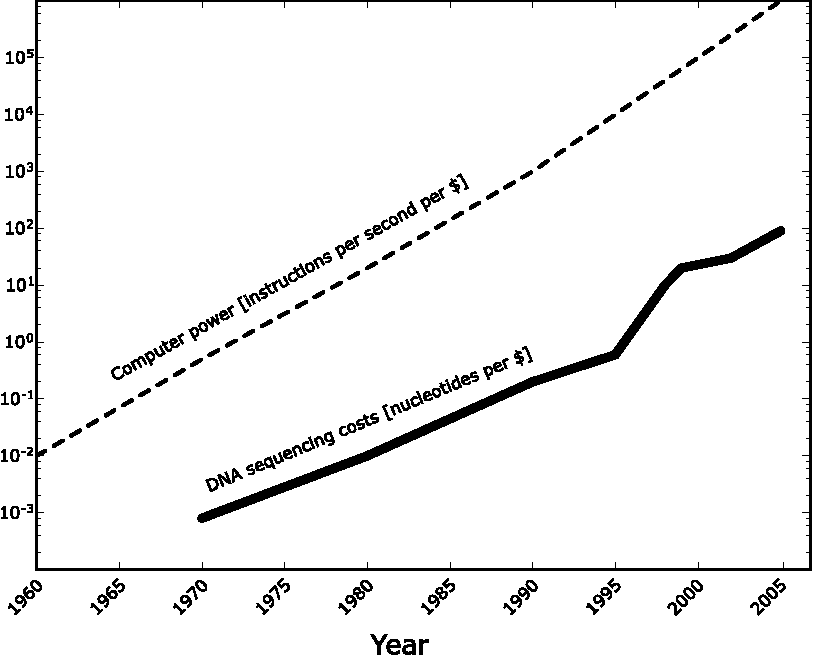
\includegraphics[width=\textwidth]{Body/Images-chap1/moore.pdf}
            \caption[Exponential growth of sequencing throughput]{
                Exponential growth of sequencing throughput~\cite{shendure2004advanced}.  The
                figure tracks the number of nucleotides that can be
                sequenced for a dollar over time juxtaposed with the
                advancement of computing power.  The hypothesis
                referred to as ``Moore's Law'' --- that
                computational power doubles every 18 months ---
                appears somewhat applicable to DNA sequencing.
                Engineering advancements in the basic
                electrophoretic method of DNA sequencing, the
                so--called ``Sanger sequencing,'' over the past 30 years
                decreased the cost of sequencing many--fold.  During
                the 15 year Human Genome Project, widespread
                investment into innovation and automation drove down the
                cost tenfold, greatly accelerating
                the completion of the project ---
                85\% of the genome was sequenced in the project's last
                two years~\cite{collins2003human}.
        }
            \label{fig:moore}
            \end{figure}

           \begin{figure}[ptb]
            \centering
            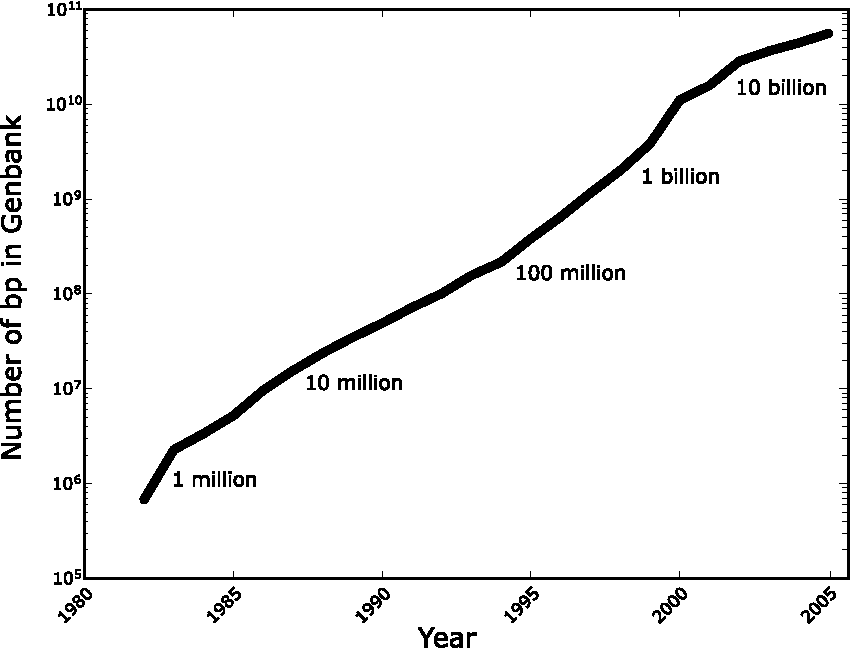
\includegraphics[width=\textwidth]{Body/Images-chap1/genbank.pdf}
            \caption[Exponential growth of Genbank]{Exponential
            growth of Genbank~\cite{benson2006genbank}.  Genbank is
            a comprehensive database of DNA sequences from over 200,000
            organisms that were made public by direct
            submission from researchers.  The database is maintained
            by the U.S. National Center for Biotechnology Information, and is updated daily.  The sequences in Genbank
            include data from genome sequencing projects, expressed
            sequence tags, and international sequence data from the
            European Molecular Biology Laboratory and the DNA
            Databank of Japan.  Genbank receives over 1000
            submissions per day and has doubled roughly every 18
            months since being started.  It is the largest database
            of its kind and is the basis for many
            ``information--added'' databases and resources.
            See also~\vref{fig:moore}.
        }
            \label{fig:genbank}
            \end{figure}


This torrent of data is not restricted to DNA sequencing.
Technological advances in recent years produced myriad tools
for quantifying biology including DNA microarrays, reverse
transcriptase polymerase chain reaction (RT--PCR), flow cytometry,
chromatin--immunoprecipitation (chip--chip), yeast two--hybrid
assays, fluorescence and confocal microscopy, generalized robotic
screening methods, and countless others.  These tools enable the
continual coining of new ``omes'' such as the transcriptome,
proteome, and interactome --- high--throughput counterparts to
traditional areas of study in biology.  (See Figure~\vref{fig:omes}
and Table~\vref{table:omes}.)  These new fields do not exist in
isolation, but instead contribute to an ever--increasing network of
information.  Consider the Genbank annotation of the human insulin
gene as shown an Figure~\vref{fig:genbank-record}. The annotation
includes detailed information about insulin culled from the
scientific literature by human experts including not just the
sequence of the gene, but also its post--translational
modifications, cellular localization, interactions with other genes,
role in energy metabolism and diabetes, and numerous links to
external databases with yet more information.

            \begin{figure}[ptb]
            \centering
            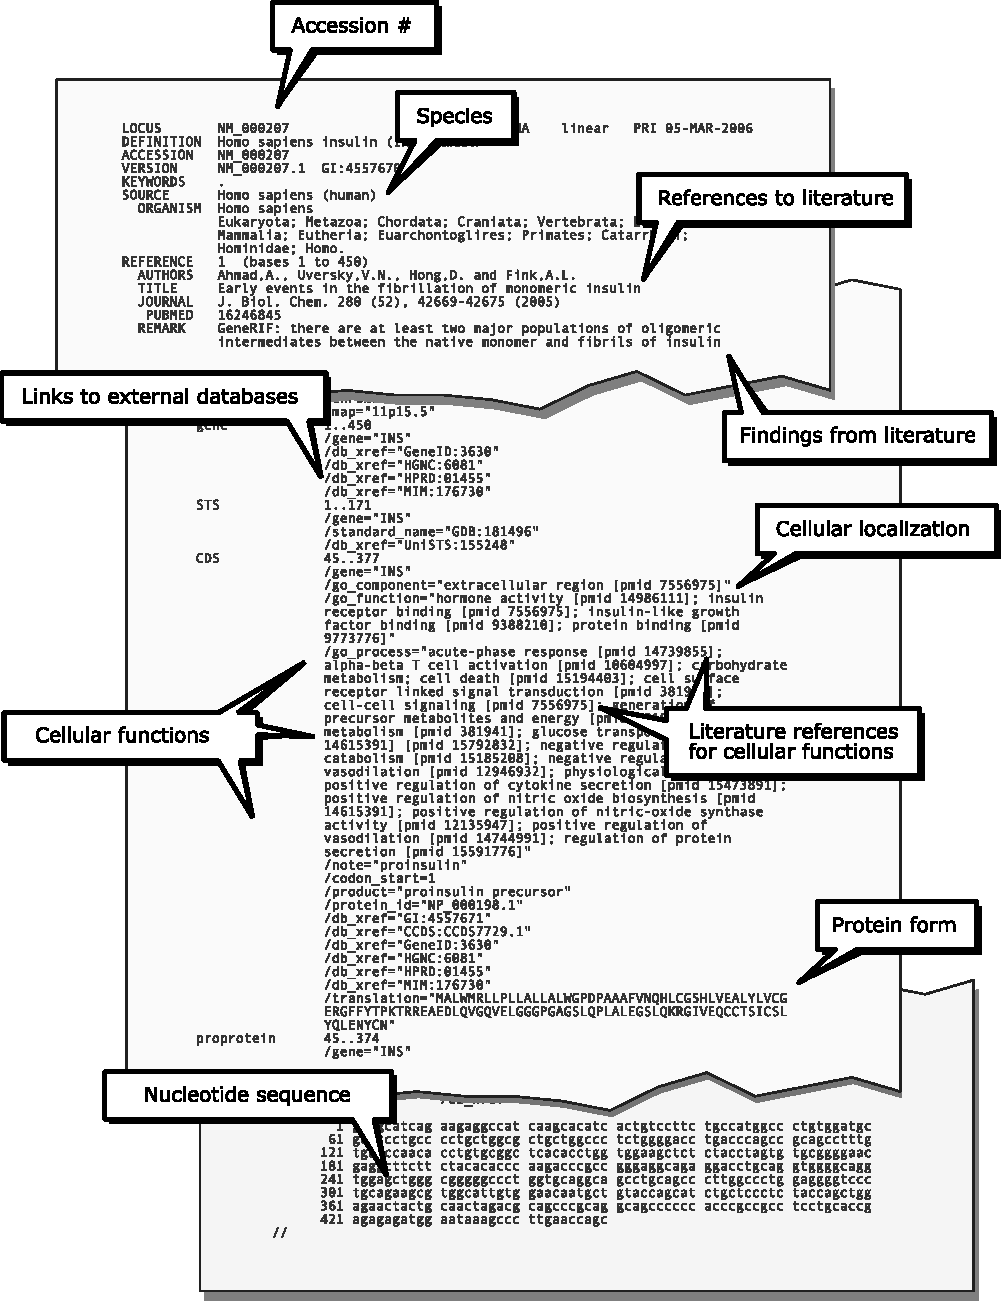
\includegraphics[width=0.90\textwidth]{Body/Images-chap1/genbank-record.pdf}
            \caption[A sample Genbank record]{A sample Genbank
            record showing the litany of features annotating the
            human gene for insulin.  As the figure suggests, this
            ``extra'' information typically dwarfs the gene sequence
            in size.  The annotations are highly cross--referenced,
            linking genes to cellular functions, behaviors,
            localizations and to other databases with yet more
            information.  Viewed \emph{en masse}, a complex network
            of knowledge emerges linking primary sequences
            into the understanding of higher--order systems at the
            cellular, tissue, an organism levels.
        }
            \label{fig:genbank-record}
            \end{figure}







\begin{table}
    \caption[``Omic'' fields other than genomic and proteomic]{
        ``Omic'' fields other than genomic and proteomic.
        In many cases, fields have been reborn as ``omic''
        fields due to a changing focus towards higher throughput
        empirical methods.  This list is indicative of the shift
        in biology towards quantitation and the resulting need
        for new, automated modes of analysis.  The rise
        of these words over time in the scientific vernacular
        is shown in Figure~\vref{fig:omes}.
        This list
        was compiled by searching over 5 million articles in the
        life sciences literature using the NCBI eutils
        API~\cite{ncbi2005eutils}.
        See also references in the
    bibliography~\cite{gerstein2005omes,dana2005omics}.
        }\label{table:omes}
	\centering
    \begin{tabular}{llll} \hline \hline
    Anatomics
    & Biomics
    & Chromosomics
    & Cytomics \\
     Enviromics
    & Epigenomics
    & Fluxomics
    & Glycomics \\
     Glycoproteomics
    & Immunogenomics
    & Immunomics
    & Immunoproteomics \\
     Integromics
    & Interactomics
    & Ionomics
    & Lipidomics \\
     Metabolomics
    & Metabonomics
    & Metagenomics
    & Metallomics  \\
     Metalloproteomics
    & Methylomics
    & Mitogenomics
    & Neuromics \\
     Neuropeptidomics
    & Oncogenomics
    & Peptidomics
    & Phenomics  \\
     Phospho-proteomics
    & Phosphoproteomics
    & Physiomics
    & Physionomics  \\
     Post--genomics
    & Postgenomics
    & Pre--genomics
    & Rnomics \\
     Secretomics
    & Subproteomics
    & Surfaceomics
    & Syndromics \\
     Transcriptomics \\ \hline \hline
    \end{tabular}
\end{table}



\begin{figure}
    \centering
    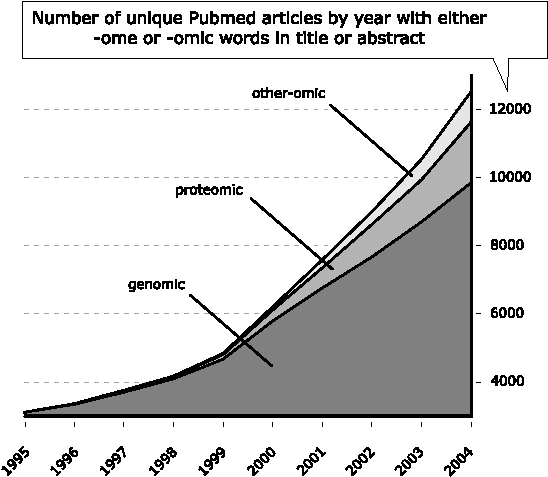
\includegraphics[width=0.8\textwidth]{Body/Images-chap1/omes.pdf}
    \caption[Usage of ``ome'' and ``omic'' words over time]{
            Usage of ``ome'' and ``omic'' words over time divided
            into three catagories: genome and genomic, proteome
            and proteomic, and other ome and omic.  The latter
            category comprises those words shown in
            Table~\vref{table:omes}.
    }\label{fig:omes}
\end{figure}



The Genbank annotation of insulin is the rule rather than the
exception.  It is a small piece of the growing wealth of data
describing life processes from the molecular level all the way to
the organism and ecological levels.  However, inasmuch as these data
hold promise, they also present challenges: if our ability to
collect data has increased exponentially, has our ability to
interpret and derive meaningful conclusions from these data kept
track? Will these diverse data allow us to ``connect the dots,'' to
reveal rich systems--level information? Or, instead, are they
subject to the law of diminishing returns? The prevailing punditry
lends credence to the former: witness the rise of systems
biology~\cite{ideker2003building,hwang2005data,salazar2006bioinformatics}.

But the problem remains: how can the potential of these volumous and diverse data sets
be realized?  The sheer amount of data points to the need for
automated, computational methods for analysis.  This need is driving
the co--opting of computer science as a core discipline of biology.
That is, computational methods are becoming increasingly necessary
to analyze the vast data sets biologists have accrued, and
consequently, computer science and mathematics are becoming as
fundamental to biology as chemistry and physics.  The particular
sub--discipline of biology devoted to these computational methods is
typically referred to as either bioinformatics or computational
biology.  Together, these fields comprise many research topics
devoted to both data analysis and modeling of biological systems.

It is likely that the need for automated, computational analysis
will only increase in the future. There are 334 completely sequenced
genomes and over 700 genomes in various stages of completion in the
genome database at the U.S. National Center for Biotechnology
Information (NCBI)~\cite{wheeler2006database}. But, of the finished
genomes, only two are mammalian: \emph{Homo
sapiens}~\cite{venter2001sequence,lander2001initial} and \emph{Mus
musculus}~\cite{waterston2002initial}, human and mouse. This
suggests that, rather than being in the ``post--genomic'' age, we
have just begun the genomic age. Upcoming years will see the
completion of many genomes with relevance to human health and
disease --- such as the rat, rabbit, and chimpanzee genomes --- and
to industry such as the cow, corn, and potato genomes.  Furthermore,
these are just the sequencing data.  Analogous progress in fields
such as metabolomics and proteomics is likely to leave biologists
awash in data, further exacerbating the need for automated methods
of interpreting and modeling these data.


The motivation for automated data analysis techniques that I have
painted in this introduction is quite broad, but what remains of
this thesis is not. The focus of the remainder is automated,
computational methods for discovering motifs in sequential data such
as DNA and protein sequences.  For example, imagine a scenario in
which we would like to correlate one of the annotations of insulin
shown in Figure~\ref{fig:genbank-record} to a particular part of the
DNA that encodes insulin. This is a very common problem in
bioinformatics.  In essence, this is like trying to learn a language
we don't speak by reading many books.  As suggested by
Figure~\vref{table:arabGenes}, this is a nontrivial problem.


                \begin{table}[!hbtp]
                \centering
                \caption[Gene sequences from \emph{Arabodopsis thaliana}]{Genes sequences from \emph{Arabodopsis thaliana},
                a popular plant model organism.  These very small genes are only a
                few hundred bases long, whereas a typical gene can be many kilo--bases in length.
                Given these sequences, how can we find all the small repeated
                motifs such as \texttt{CCACGCGTCCGAAAA}?  At a glance, the task seems
                difficult.
                Digging further it seems insurmountable --- the
                sequences below are just a small snippet of Genbank .  To
                print just the nucleotide sequences in Genbank
                using this font would require 30 million pages: a stack of
                paper 3 km high, or roughly the distance from MIT to
                Harvard.}\label{table:arabGenes}
                    \begin{tabular}{l}\hline\hline
$>$gi$\|$8571926 Arabidopsis thaliana lipid transfer protein \\
\ttfamily \footnotesize CCACGCGTCCGAAAAAAAAAACAGAAAGTAACATGAGATCTCTCTTATTAGCCGTGTGCCTGGTTCTTGC \\
\ttfamily \footnotesize TTTACACTGCGGTGAAGCAGCCGTGTCTTGCAACACGGTGATTGCGGATCTTTACCCTTGCTTATCCTAC \\
\ttfamily \footnotesize GTGACTCAGGGCGGACCGGTCCCAACCCTCTGCTGCAACGGTCTCACAACACTCAAGAGTCAGGCTCAAA \\
\ttfamily \footnotesize CTTCTGTGGACCGTCAGGGGGTCTGTCGTTGCATCAAATCTGCTATTGGAGGACTCACTCTCTCTCCTAG \\
\ttfamily \footnotesize AACCATCCAAAATGCTTTGGAATTGCCTTCTAAATGTGGTGTCGATCTCCCTTACAAGTTCAGCCCTTCC \\
\ttfamily \footnotesize ACTGACTGCGACAGTATCCAGTGAGACAAGCAGAAAATCTTAAAGGAAGCTACTACAAGAACTATAATAA \\
\ttfamily \footnotesize CCTAATAATTAATAAATGAGGGCATTGGTTTGCTAGTTGCTAATTGATCAGTGATGTATTGTCATTTTGA \\
\ttfamily \footnotesize ATGTTCTAATATCAGCAGGCACTTATCTCTGAAAAAAAAAAAAAAAA \\ \\
$>$gi$\|$8571922 Arabidopsis thaliana lipid transfer protein \\
\ttfamily \footnotesize CCACGCGTCCGAAAACACAAGCGTAGAAAACAAAACTCAACTAATTGTGTTATCACCCAAAAGAGAAGAG \\
\ttfamily \footnotesize CAAACACAATGGCTTTCGCTTTGAGGTTCTTCACATGCTTTGTTTTGACAGTGTTCATCGTTGCATCAGT \\
\ttfamily \footnotesize GGATGCAGCAATAACATGTGGCACAGTGGCAAGTAGCTTGAGTCCATGTCTAGGCTACCTATCGAAGGGT \\
\ttfamily \footnotesize GGGGTGGTGCCACCTCCGTGCTGTGCAGGAGTCAAAAAGTTGAACGGTATGGCTCAAACCACACCCGACC \\
\ttfamily \footnotesize GCCAACAAGCATGCAGATGCTTACAGTCCGCTGCAAAAGGGGTTAATCCAAGTCTAGCCTCTGGCCTTCC \\
\ttfamily \footnotesize TGGAAAGTGCGGTGTTAGCATCCCCTATCCCATCTCCACGAGCACCAACTGCGCCACCATCAAGTGAAGT \\
\ttfamily \footnotesize GGGGAATAACGACATCATTTGCCTGAAGAGTATGGTTTCGTATACGTAAAATAAGACGGCTATCTAAGCT \\
\ttfamily \footnotesize GATATTTACCTTGTCTTTGTTTGTCTTGATGGCTTTGTAATCTTTTGCTTTGTTATGTTGTATACTTGTG \\
\ttfamily \footnotesize TCTTAACATGTTTAAGATATGATAATATATAGTATCGGTACCTTATTAAAAAAAAAAAAAAA \\ \\
$>$gi$\|$8571922 Arabidopsis thaliana lipid transfer protein \\
\ttfamily \footnotesize CCACGCGTCCGAAAACACAAGCGTAGAAAACAAAACTCAACTAATTGTGTTATCACCCAAAAGAGAAGAG \\
\ttfamily \footnotesize CAAACACAATGGCTTTCGCTTTGAGGTTCTTCACATGCTTTGTTTTGACAGTGTTCATCGTTGCATCAGT \\
\ttfamily \footnotesize GGATGCAGCAATAACATGTGGCACAGTGGCAAGTAGCTTGAGTCCATGTCTAGGCTACCTATCGAAGGGT \\
\ttfamily \footnotesize GGGGTGGTGCCACCTCCGTGCTGTGCAGGAGTCAAAAAGTTGAACGGTATGGCTCAAACCACACCCGACC \\
\ttfamily \footnotesize GCCAACAAGCATGCAGATGCTTACAGTCCGCTGCAAAAGGGGTTAATCCAAGTCTAGCCTCTGGCCTTCC \\
\ttfamily \footnotesize TGGAAAGTGCGGTGTTAGCATCCCCTATCCCATCTCCACGAGCACCAACTGCGCCACCATCAAGTGAAGT \\
\ttfamily \footnotesize GGGGAATAACGACATCATTTGCCTGAAGAGTATGGTTTCGTATACGTAAAATAAGACGGCTATCTAAGCT \\
\ttfamily \footnotesize GATATTTACCTTGTCTTTGTTTGTCTTGATGGCTTTGTAATCTTTTGCTTTGTTATGTTGTATACTTGTG \\
\ttfamily \footnotesize TCTTAACATGTTTAAGATATGATAATATATAGTATCGGTACCTTATTAAAAAAAAAAAAAAA \\\hline\hline
\end{tabular}

                \end{table}

Motif discovery in sequential data is only one tiny sliver of the
vast spectrum of topics spanned by bioinformatics and computational
biology. However, many of the principles and tools I describe have
broader implications for learning and automated discovery methods in
biology.  Chapter 1 of this thesis is devoted to familiarizing the
reader with basic concepts of motif discovery, with a particular
focus on linguistic methods of modeling sequences. In Chapter 2,
these concepts are applied to the annotation and design of novel
antibiotics, called antimicrobial peptides.  The principal
contribution of this thesis is the third chapter, in which I develop
a framework and software tool for motif discovery that can be
generalized to diverse types of data and is superior to existing
tools in many ways.  Finally, the last chapter comprises a series of
vignettes that take a more broad approach to motif discovery and
explore a number of issues adjoining the central theme of the first
three chapters.

\section{Fundamental tenets of motif discovery}\label{section:tenents}

I will begin with a series of elementary, almost philosophical
examples that serve to illustrate some of the fundamental tenets of
motif discovery. These examples may seem pedantic; however, the
tenets they illustrate will be recurring themes throughout this
thesis. Further, the following sections will serve to establish a
common vocabulary and mode of thought that will enable the
development of more complex ideas in later chapters.

In the most basic sense, the task of motif discovery is to find a
repeated feature in a data set.  Take, for example, the objects below.


\begin{equation}\label{eqn:shapes}
    \blacksquare\blacktriangle\square\blacksquare
\end{equation}



What features are repeated at least twice in the objects?  One
answer is that the square shape appears three times.  Yet another,
is that three of the objects are darkened.  And finally, a more
sophisticated answer is that all of the objects are regular
polyhedrons.  Which of these is correct? All three are.  The first
two answers are intuitively obvious, whereas the final answer is
rooted in a knowledge of geometry.  The degree to which one answer
is ``more correct'' than the others depends on what kinds of
features we are interested in \emph{a priori}.  This is the first
and most important tenet of motif discovery.


Consider a second question: is the dark square more similar to the
dark triangle or to the hollow square?

\begin{equation}\label{eqn:shapes2}
    \blacksquare\sim\blacktriangle\sim\square
\end{equation}

Again, there is no correct answer. The response obviously depends on
our relative preference for color versus shape.  This variety of
question is even more difficult when we seek to quantify the degree
of similarity or difference --- the distance --- between two
objects.  Is a human more similar to an alligator, or to an
elephant? Based on body temperature, the human is more similar to
the elephant; however, based on weight, the opposite true.  This is
the second tenet of motif discovery: the measurement of
``distance'' between objects is inherently relative, or dependent on
predefined metrics.

Now consider a more complicated example shown schematically in
Figure~\vref{fig:gaussian}.  The figure shows an X--Y scatter plot
with 12 data points.  How many groups of points, or clusters, are in
this figure?  As before, there are many correct answers: three
groups of four; one group of four and one group of eight; or one
single group of twelve.  The answer depends on our preconceived
notion of how small the distance between objects must be in order
for them to be grouped together.  Or, equivalently, how similar
objects must be to be considered the same.  This is our third and final
tenet of motif discovery.

            \begin{figure}[ptb]
            \centering
            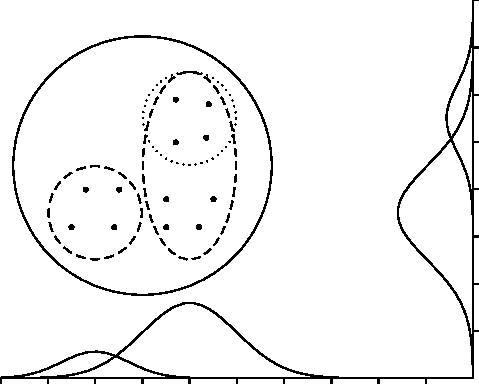
\includegraphics[width=\textwidth]{Body/Images-chap1/gaussian.pdf}
            \caption[Finding patterns in generic data]{Clustering to find patterns in generic data.  Given this data set,
            we would cluster the data together to find patterns (indicated here by the ellipses).  But, there are many different
            patterns we could find.  Which ones are correct?}
            \label{fig:gaussian}
            \end{figure}

The three tenets we have just developed can be rephrased as follows.
The answer to any motif discovery problem will always depend on what
kinds of motifs we are looking for and the search for these motifs
will always depend on a predefined metric of similarity and method
for grouping together similar objects.

\section{Motif discovery in sequential data}


In this section, I define ``sequential data'' and introduce some
basic concepts of motif discovery in sequential data.  I will build
upon tenets developed in the previous section and develop more
complex ideas in motif discovery that are specific to sequential
data.

In the most general sense, sequential data are any data in which
there is a natural ordering, such that rearranging the data would
result in lost information.  In later chapters, we will deal with
the more general case of sequential data that encompasses series of
multidimensional real--valued data; however, for the time being, we
can consider sequential data to be a series of alphanumerical
characters such as the four sequences shown below.

\begin{multline}\label{eqn:lincoln1}
   \texttt{djndfduckdeicfjnfmABRAHAMLINCOLN}\\
   \texttt{idkeioddsnABRAHAMLINCOLNaknkwbad}\\
   \texttt{ioxcABRAHAMLINCOLNabkjwlkdaxlakj}\\
   \texttt{xkasnkjlfABRAHAMLINCOLNkdsjkjsdl}
\end{multline}



    We can refer to these sequences more formally by calling the set
    of sequences $S$, where $S$ is defined such that
     $S=\braces{s_0,s_1,s_2,\ldots,s_n}$, and where
    sequence $s_i$ has length $W_i$.  So, in the above example, $n=3$
    and $s_0=\texttt{djndfduckdeicfjnfmABRAHAMLINCOLN}$.  Furthermore, let
    the
    the $\ith{j}$ member of the $\ith{i}$ sequence
    be denoted by $s_{i,j}$.
    So, $s_{0,0}=d$, $s_{0,1}=j$, etc.
    Each $s_{i,j}$ is a
    primitive, or atomic unit, for the data that is
    being analyzed.  For now, we will say that the primitives
    are alphanumerical characters selected from some alphabet
    $\Sigma$.  In the example above, this alphabet is the set of 52
    lowercase and uppercase characters from the Roman alphabet.
    However, this alphabet can be defined in many different ways
    depending on the context of our motif discovery problem.  For
    example, for a DNA sequence the alphabet would
    comprise the characters $\{\texttt{A,T,G,C}\}$, representing the
    four bases found in DNA: adenosine, thymine, guanine, and
    cytosine (see Figure~\vref{fig:bases} in the Appendix.  Or, for protein sequences,
    the alphabet would be the
    set of characters representing the one letter abbreviations for
    the 20 naturally occurring amino acids
    $\{\texttt{A,R,N,D,C,Q,E,G,H,I,L,K,M,F,P,S,T,W,Y,V}\}$, which
    are defined in Figure~\vref{fig:aas} in the Appendix.


In the set of sequences above, the motif ``\texttt{ABRAHAMLINCOLN}''
is inherently obvious in the otherwise random series of characters
that make up each of the individual sequences.  A similar motif is
obvious even when the sequences are ``mutated'' as shown below.



\begin{align}\label{eqn:lincoln2}
   s_0 &= \texttt{djndfduckdeicfjnfmABELINCOLN}\\
   s_1 &= \texttt{idkeioddsnABRAHAMLINCOLNaknkwbad}\notag\\
   s_2 &= \texttt{ioxcALINCOLNabkjwlkdaxlakj} \notag\\
   s_3 &= \texttt{xkasnkjlfABRAHAMLINCOLNkdsjkjsdl}\notag
\end{align}

In two of these sequences, Abraham is abbreviated but is still
recognizable.  But now, it is not appropriate to call the motif
simply ``\texttt{ABRAHAMLINCOLN}.''  At this point, it is important
to develop a more rigorous definition of ``motif'' that will allow
us to describe all the possible permutations shown in the above
mutated sequences.  A motif is, henceforth, a mathematical model
used to describe a set of locations in a set of sequences.  These
locations are referred to as ``motif instances.''  In the example
above, the motif instances are the substrings:
``\texttt{ABELINCOLN},'' ``\texttt{ABRAHAMLINCOLN},''
``\texttt{ALINCOLN},'' and ``\texttt{ABRAHAMLINCOLN}'' in sequences
$s_0$, $s_1$, $s_2$, and $s_3$, respectively.

Any mathematical model used to describe these instances should say
that each instance begins with the letter \texttt{A}, optionally
followed by either \texttt{BE} or \texttt{BRAHAM}, and necessarily
followed by \texttt{LINCOLN}.  That is, a model that describes the
ordered arrangement of objects, in this case characters.  Such
models are commonplace in the field of linguistics and are called
grammars.

\section{Grammatical models of sequences}


\subsection*{Introduction}

The theory underlying grammatical models of sequences can be traced
back to Noam Chomsky's early work on syntax
theory~\cite{chomsky1957syntactic,chomsky1965aspects,chomsky1956three}.
 Chomsky's work is the basis for much of formal language theory and
computational linguistics.  However, in general, most research in these
areas has used grammars for pattern \emph{recognition} vice pattern
\emph{discovery}, and focuses on machine learning techniques for
computer understanding of natural languages. Only recently have
these pattern recognition techniques been applied to problems of
interest to
biologists~\cite{searls1997linguistic,searls2001reading,searls1992thecomputational}.

As I will show in the following sections, most motif discovery
algorithms in bioinformatics use motif models that can be reduced,
in general, to a grammatical model.  However, for the most part,
such reductions are rare in the bioinformatics literature. This is
because motif discovery and bioinformatics evolved independently
from formal language theory.  In a sense, the two fields are distant
homologs of each other, both making use of models that can be
reduced to grammars.


A grammar is a mathematical construct that describes the ordered
arrangement of objects, usually words or characters, in a
sequence~\cite{aho1979theory}.
 More rigorously, a grammar is a 4--tuple $G = (N,\Sigma,P,S) $
 wherein
\begin{enumerate}\label{grammarDefinition}
  \item $N$ is a finite set of non-terminal symbols, also called
  variables or syntactic categories;
  \item $\Sigma$ is a finite set of terminal symbols, disjoint from
  $N$;
  \item $P$ is a finite subset of
    \begin{equation}\label{eqn:production}
        (N\cup\Sigma)*N(N\cup\Sigma)*\times(N\cup\Sigma)*,
    \end{equation}
    each element in $P$ is called a ``production'' and
    is written in the form $\alpha\rightarrow\beta$%
    \footnote{The star symbol, $*$, is called the Kleene star and is
    interpreted as ``zero or more'' of the expression it follows.
    For example, \texttt{ZA*} would be interpreted as a \texttt{Z}
    followed by zero or more \texttt{A} characters.  The Kleene star
    and other similar operators will be discussed later in the
    section on regular grammars and regular expressions\vref{section:regex}.
    }; and,
    \item $S$ is a special symbol in $N$ that is the start symbol.
\end{enumerate}

To illustrate how a grammar can be used to model sequences, consider
the following simple grammar:

\begin{equation}\label{eqn:simpleGrammar}
    G = (\{\alpha, S\},\{\texttt{0}, \texttt{1}\},P,S),
\end{equation}

where the set of productions, $P$, is given by

\begin{align}\label{eqn:simpleProduction}
    P =
    \begin{cases}
    S \rightarrow \texttt{0}\alpha \texttt{1}\\
    \texttt{0}\alpha \rightarrow \texttt{00}\alpha \texttt{1}\\
    \alpha \rightarrow e.
    \end{cases}
\end{align}

Each line in the set of productions is essentially a replacement
rule. For example, the operation $S \rightarrow \texttt{0}\alpha
\texttt{1}$ should be read as ``replace the character $S$ with the
sequence of characters $\texttt{0}\alpha \texttt{1}$.''  Then, the
subsequent line should be read as ``replace the two character
sequence $\texttt{0}\alpha$ with the sequence $\texttt{00}\alpha
\texttt{1}$.''  Finally, the last production should be read as
``replace the character $\alpha $ with the character $e$, which is
the termination character.''  These productions follow a few
conventions that are used throughout this manuscript.  First, as
defined on page~\pageref{grammarDefinition}, $S$ is a special
non--terminal symbol that is always used as the starting symbol.
Second, in order to distinguish terminal symbols from non--terminal
symbols, the former will always be displayed in a fixed width font.
Third, the
character $e $ is used always to represent the termination of a
sequence and is referred to as the termination character.

Now consider how to construct a sequence using the set of
productions in the grammar shown in
Equations~\ref{eqn:simpleGrammar} and~\ref{eqn:simpleProduction}.  Starting
with the special non--terminal character $S$, the first production
produces a three letter sequence.
\begin{align*}
    S &\Rightarrow \texttt{0}\alpha \texttt{1}
\end{align*}
Using the second production, produces a four character sequence.
\begin{align*}
    S &\Rightarrow \texttt{0}\alpha \texttt{1}  \Rightarrow \texttt{00}\alpha \texttt{1}
\end{align*}
Finally, using the third production terminates the sequence.
\begin{align}\label{eqn:simpleDerivation}
    S \Rightarrow \texttt{0}\alpha \texttt{1}  \Rightarrow \texttt{00}\alpha \texttt{1}
    \Rightarrow \texttt{001}
\end{align}

The sequences produced by following the production rules of the
grammar are called derivations of a grammar, or equivalently the
sentences or sentenial forms of the grammar.  The collection of
sentenial forms of a grammar are collectively called the language
generated by $G$, or $L(G)$.

Notably, the final sequence shown in
Equation~\ref{eqn:simpleDerivation} is not the only sequence that
can be derived from the grammar $G$.  Because the symbol
$\alpha$ appears in two different productions, either production can
be used and neither production is preferred \emph{a priori}.  For
example the following sequence is an equally valid derivation of the
same grammar.
\begin{align}\label{eqn:simpleDerivation2}
    S \Rightarrow \texttt{0}\alpha \texttt{1}  \Rightarrow \texttt{00}\alpha \texttt{1}
    \Rightarrow \texttt{000}\alpha \texttt{1}
    \Rightarrow \texttt{0000}\alpha \texttt{1}
    \Rightarrow \texttt{00000}\alpha \texttt{1}
    \Rightarrow \texttt{00000}\texttt{1}
\end{align}
As the derivation above suggests, any sequence that
\begin{itemize}
  \item begins with a \texttt{0},
  \item that is followed by zero or more \texttt{0}s, and
  \item is terminated by a single \texttt{1}
\end{itemize}
could be a derivation of the grammar shown in
Equation~\vref{eqn:simpleGrammar}. Collectively, these derivations
form the language of the grammar.


Now I will return to the Abraham Lincoln example shown in
Equation~\vref{eqn:lincoln2}.  Recall that the motif instances are
the substrings ``\texttt{ABELINCOLN},'' ``\texttt{ABRAHAMLINCOLN},''
``\texttt{ALINCOLN},'' and ``\texttt{ABRAHAMLINCOLN}'' in sequences
$s_0$, $s_1$, $s_2$, and $s_3$, respectively.  A grammar that
describes these motif instances is
\begin{equation}\label{eqn:abeGrammar}
    G = (\{\alpha, S\},\{\texttt{A}, \texttt{B}, \texttt{C},\texttt{E}, \texttt{H}, \texttt{I},
    \texttt{L}, \texttt{M}, \texttt{N}, \texttt{R}\},P,S),
\end{equation}
where $P$ is given by the set of productions
\begin{align}\label{eqn:abeProduction}
    P =
    \begin{cases}
    S \rightarrow \texttt{A}\alpha \\
    \alpha \rightarrow \beta \\
    \alpha \rightarrow \texttt{BE}\beta \\
    \alpha \rightarrow \texttt{BRAHAM}\beta \\
    \beta \rightarrow \texttt{LINCOLN}\gamma \\
    \gamma \rightarrow e.
    \end{cases}
\end{align}


Again, in a manner similar to Equation~\vref{eqn:simpleProduction},
the grammar shown in Equation~\vref{eqn:abeProduction} has a
non--terminal character, $\alpha$, in multiple productions.  In such
cases, the production can usually be abbreviated using the ``$\mid$''
character, which is to be read as ``or.''  For example, the
productions in Equation~\vref{eqn:abeProduction} can be written
equivalently as
\begin{align}\label{eqn:abeProduction2}
    P =
    \begin{cases}
    S \rightarrow \texttt{A}\alpha \\
    \alpha \rightarrow \beta \mid \texttt{BE}\beta \mid \texttt{BRAHAM}\beta \\
    \beta \rightarrow \texttt{LINCOLN}\gamma \\
    \gamma \rightarrow e.
    \end{cases}
\end{align}

Notice that the grammar shown in Equation~\vref{eqn:abeProduction}
describes exactly all four of the motif instances in the sequences
shown in Equation~\vref{eqn:lincoln2}.  The three possible
derivations of the grammar are shown below.
\begin{align}\label{eqn:abeDerivation}
    S \Rightarrow \texttt{A}\alpha   \Rightarrow \texttt{A}\beta
         \Rightarrow \texttt{ALINCOLN}\gamma  \Rightarrow
        \texttt{ALINCOLN}\\
    S \Rightarrow \texttt{A}\alpha   \Rightarrow \texttt{ABE}\beta
         \Rightarrow \texttt{ABELINCOLN}\gamma  \Rightarrow
        \texttt{ABELINCOLN}\notag\\
    S \Rightarrow \texttt{A}\alpha   \Rightarrow \texttt{ABRAHAM}\beta
        \Rightarrow \texttt{ABRAHAMLINCOLN}\gamma  \Rightarrow
        \texttt{ABRAHAMLINCOLN}\notag
\end{align}

This is an ideal case.  In general, in constructing any model
describing any motif instances, we would like to use a grammar that
is sensitive for the instances
--- i.e.\ all the instances are derivations of $G$ --- and specific
for the instances --- i.e.\ the language $L (G)$ includes few
derivations that are not motif instances.

Now consider a more complicated case in which a grammar is used to
model DNA sequences that are likely to assume a hairpin structure,
such as those shown in Figure~\vref{fig:hairpin}.  Hairpins in DNA
and RNA sequences play an important role in the regulation of many
processes, including transcription and translation.  A hairpin is
essentially a structure that bends back upon itself and is held
together by Watson--Crick pairing.  The paired bases in the hairpin
structure are referred to as the ``stem'' and the unpaired, bulging
bases are referred to as the ``loop'' (see
Figure~\vref{fig:hairpin}).

            \begin{figure}[ptb]
            \centering
            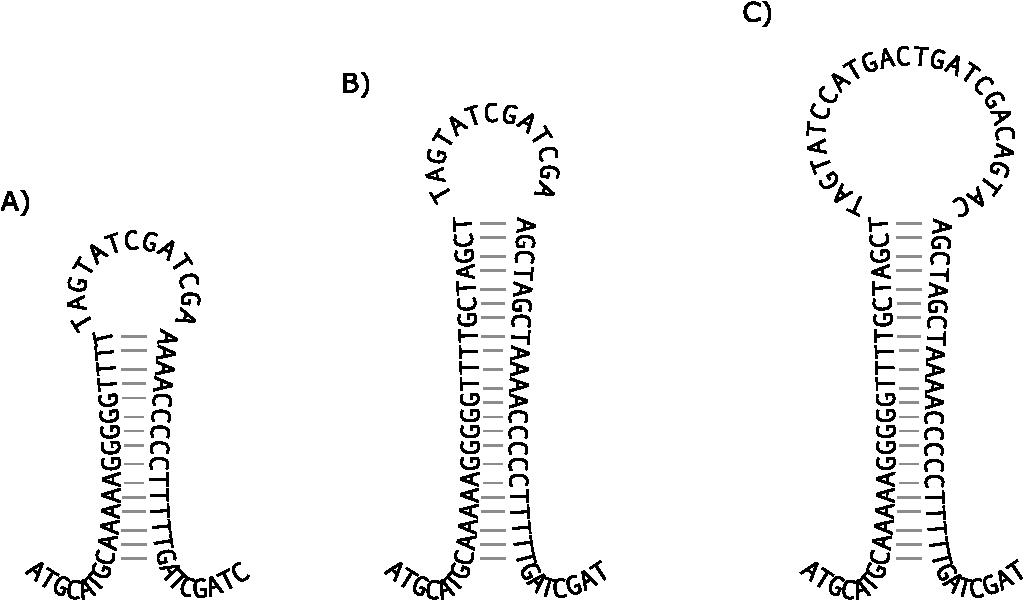
\includegraphics[width=\textwidth]{Body/Images-chap1/hairpin.pdf}
            \caption[Hairpin loops in DNA secondary structures]{
            Hairpin loops in DNA secondary structures.  A hairpin
            loop is a secondary structure in a sequence containing two
            regions that are reverse complements of each other.
            These regions form the ``stem'' of the hairpin loop.
            The figure shows three hairpin loops in which the stem
            size gets progressively larger.  Also notice that, the
            bulbous region --- the ``loop'' --- which is not paired
            with any other region, can be of arbitrary size.  The
            structures play an important part in the regulation of
            DNA transcription and, for RNA, in the process of
            translation.
            }
            \label{fig:hairpin}
            \end{figure}

In order to form a stem--loop, or hairpin structure, the two
sequences in the stem must be reverse complements of each other.
This type of relationship is captured in the following grammar:
\begin{equation}\label{eqn:hairpinGrammar}
    G = (\{\alpha, \beta, S\},\{\texttt{A}, \texttt{G},\texttt{T},\texttt{C}\},P,S),
\end{equation}
where $P$ is given by
\begin{align}\label{eqn:hairpinProduction}
    P =
    \begin{cases}
    S \rightarrow \alpha \\
    \alpha \rightarrow \texttt{A}\alpha\texttt{T} \mid \texttt{T}\alpha\texttt{A} \\
    \alpha \rightarrow \texttt{G}\alpha\texttt{C} \mid \texttt{C}\alpha\texttt{G} \\
    \alpha \rightarrow \beta \mid e \\
    \beta \rightarrow \texttt{A}\beta \mid \texttt{T}\beta \mid\texttt{G}\beta \mid
        \texttt{C}\beta \mid e
    \end{cases}
\end{align}


The grammar shown in Equation~\vref{eqn:hairpinGrammar} can describe
any hairpin loop in which the stem consists of one or more
complementary bases and the loop consists of zero or more bases.  For
example, consider the following derivation of the grammar.
\begin{equation}\label{eqn:hairpinDerivation}
\begin{split}
    S &\Rightarrow \alpha \\
    &\Rightarrow \texttt{A}\alpha\texttt{T} \\
        &\Rightarrow \texttt{AG}\alpha\texttt{CT} \\
        &\Rightarrow \texttt{AGG}\alpha\texttt{CCT} \\
        &\Rightarrow \texttt{AGGC}\alpha\texttt{GCCT} \\
        &\Rightarrow \texttt{AGGCT}\alpha\texttt{AGCCT} \\
        &\Rightarrow \texttt{AGGCT}\beta\texttt{AGCCT} \\
        &\Rightarrow \texttt{AGGCTA}\beta\texttt{AGCCT} \\
        &\Rightarrow \texttt{AGGCTAAGCCT}
\end{split}
\end{equation}
This derivation produces a sequence that can form a hairpin
structure with a stem size of five base pairs and a loop of a single
base pair.

The grammar shown in Equation~\vref{eqn:hairpinGrammar} is more
complex than the grammar used to model the Abraham Lincoln motif
(Equation~\vref{eqn:abeGrammar}), because there are a long--range
dependencies in the sequences.  That is, a particular base produced
by the grammar in Equation~\ref{eqn:hairpinGrammar} is guaranteed
to be complementary to a base on the other side of the sequence.  In
contrast, the productions used to model the Abraham Lincoln motif
produced a set of simple derivations in a left--to--right order.
Indeed, even more complicated grammars can describe still more
long--range, complex interactions between the characters in a
sequence.


\subsection*{Hierarchy of restricted grammars}

Linguists classify grammars into four increasingly complicated
groups based on the format of their productions.  A grammar is
\begin{enumerate}
  \item right--linear, or type--3, if each production in $P$ is of the form
        $A\rightarrow \texttt{x}B$, where $A$ and $B$ are in  $N$
        and $\texttt{x}$ is any string in $\Sigma*$;\label{gramDefs}
  \item context--free, or type--2, if each production in $P$ is of the form
        $A\rightarrow \alpha$, where $A$ is in  $N$
        and $\alpha$ is  in $(N\cup\Sigma)*$;
  \item context-- sensitive, or type--1, if each production in $P$ is of the form
        $\alpha A\beta \rightarrow \delta y \Gamma$, where $A$ is in  $N$,
        $y$ is non--null, and $\alpha$,
        $\beta$, $\delta$, and $\gamma$ are  in $(N\cup\Sigma)*$;
  \item unrestricted, or type--0, if it adheres to none of these
        restrictions.
\end{enumerate}
This classification system is referred to as the Chomsky
hierarchy~\cite{chomsky1956three}. Each of these grammars defines a
corresponding class of language, which is the set of all sequences
that can be produced using a particular type of grammar.

Right--linear, or type--3 grammars are also called ``regular''
grammars and are the simplest type of grammar. These grammars are
called right--linear because derivations of these grammars are
produced stepwise from left to right, never growing from the center
of the sequence as in the derivation shown in
Equation~\ref{eqn:hairpinDerivation}.  As I will show in
Section~\vref{section:regex}, despite their simplicity, regular
grammars are the most frequently used motif model in bioinformatics.

Context--free grammars are the next most complicated class of
grammatical model.  Indeed, the hairpin grammar shown in
Equation~\vref{eqn:hairpinGrammar} is a context--free grammar.  This
type of grammar is characterized by ``nested'' dependencies (see
Figure~\ref{fig:dependencies}).  The dependencies are nested in the
sense that derivations of the grammar ``grow'' from the center, due
to the structure of the productions.


            \begin{figure}[ptb]
            \centering
            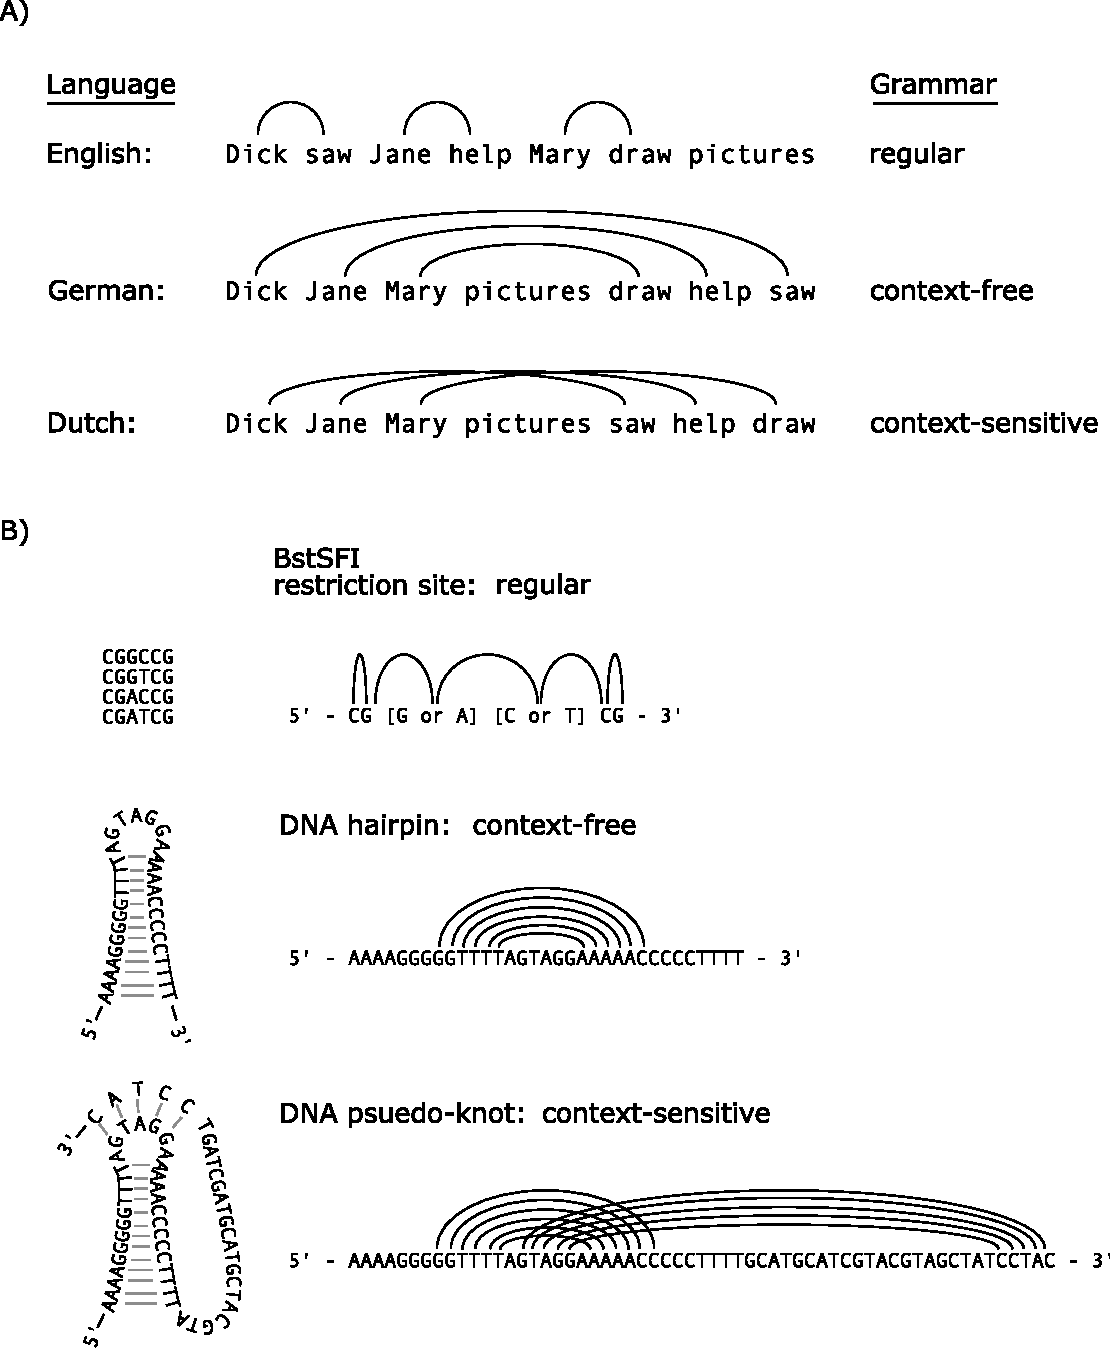
\includegraphics[width=0.80\textwidth]{Body/Images-chap1/dependencies.pdf}
            \caption[Noun--verb dependencies in various languages and their
            biological analogues]{Noun--verb dependencies in various languages and their
            biological analogues.  Part A) shows the sentence
            ``Dick saw Jane help Mary draw pictures'' translated
            grammatically into German and Dutch.  That is, the words
            in the sentence are rearranged to reflect the rules of
            grammar in these two languages, but the sentence is not
            translated \emph{per se}.  As shown, the English
            version of the sentence has a relatively simple
            dependency structure between the nouns and verbs that
            can be modeled using regular grammars.  In contrast,
            German and Dutch require more complicated grammatical
            models~\cite{shieber1985evidence,bresnan1982cross,jurafsky2000speech}.
            Part B) shows the biological analogue of the three
            sentences in Part A).  Typically, restriction sites can
            be modeled using regular grammars, whereas complex DNA
            secondary structures require context--free or
            context--sensitive grammars~\cite{rivas2000language}.  In the first example, the
            arches are used to represent a ``must be followed by''
            dependency.  In the second two examples, they represent
            a ``must be complementary to'' dependency.
            }
            \label{fig:dependencies}
            \end{figure}

Context--sensitive grammars and unrestricted grammars are the most
complex classes of grammatical models.  As shown in
Figure~\vref{fig:dependencies}, context--sensitive grammars are
characterized by long--range dependencies that are ``crossing.''
Derivations of these grammars can typically ``grow'' from anywhere
inside the sequence.  For example, consider the following grammar
that describes a card player arranging a deck of cards:
\begin{equation}\label{eqn:csGrammar}
    G = (\{\gamma, \beta, S\},\{\clubsuit, \heartsuit, \spadesuit\},P,S),
\end{equation}
where $P$ is given by
\begin{align}\label{eqn:csProduction}
    P =
    \begin{cases}
    S \rightarrow \gamma \\
    \gamma \rightarrow \clubsuit\heartsuit\spadesuit \mid \clubsuit\gamma\beta\spadesuit \\
    \spadesuit\beta \rightarrow \beta\spadesuit \\
    \heartsuit\beta \rightarrow \heartsuit\heartsuit
    \end{cases}
\end{align}

This grammar is one of the most simple context--sensitive grammars.
As well, it serves to illustrate that sequential data are not
restricted to characters \emph{per se}.  Indeed, in
Chapter~\vref{chapter:gemoda}, I will extend the definition of
sequential data to include ordered arrangements  of multidimensional
real--valued data sampled from a continuous distribution.  Returning
to the current example, consider the following derivation of this
grammar:
\begin{equation}\label{eqn:csDerivation}
    \begin{split}
    S &\Rightarrow \gamma  \\
        &\Rightarrow \clubsuit\gamma\beta\spadesuit \\
        &\Rightarrow \clubsuit\clubsuit\gamma\beta\spadesuit\beta\spadesuit \\
        &\Rightarrow \clubsuit\clubsuit\clubsuit\gamma\beta\spadesuit\beta\spadesuit\beta\spadesuit \\
        &\Rightarrow \clubsuit\clubsuit\clubsuit\clubsuit\heartsuit\spadesuit\beta\spadesuit\beta\spadesuit\beta\spadesuit \\
        &\Rightarrow \clubsuit\clubsuit\clubsuit\clubsuit\heartsuit\beta\spadesuit\spadesuit\beta\beta\spadesuit\spadesuit \\
        &\Rightarrow \clubsuit\clubsuit\clubsuit\clubsuit\heartsuit\beta\spadesuit\beta\spadesuit\beta\spadesuit\spadesuit \\
        &\Rightarrow \clubsuit\clubsuit\clubsuit\clubsuit\heartsuit\beta\spadesuit\beta\beta\spadesuit\spadesuit\spadesuit \\
        &\Rightarrow \clubsuit\clubsuit\clubsuit\clubsuit\heartsuit\beta\beta\spadesuit\beta\spadesuit\spadesuit\spadesuit \\
        &\Rightarrow \clubsuit\clubsuit\clubsuit\clubsuit\heartsuit\beta\beta\beta\spadesuit\spadesuit\spadesuit\spadesuit \\
        &\Rightarrow \clubsuit\clubsuit\clubsuit\clubsuit\heartsuit\heartsuit\beta\beta\spadesuit\spadesuit\spadesuit\spadesuit \\
        &\Rightarrow \clubsuit\clubsuit\clubsuit\clubsuit\heartsuit\heartsuit\heartsuit\beta\spadesuit\spadesuit\spadesuit\spadesuit \\
        &\Rightarrow \clubsuit\clubsuit\clubsuit\clubsuit\heartsuit\heartsuit\heartsuit\heartsuit\spadesuit\spadesuit\spadesuit\spadesuit \\
    \end{split}
\end{equation}

Notice that the derivation bears much similarity to the hairpin loop
example shown in Equation~\vref{eqn:hairpinDerivation}.  However, as
I showed earlier, hairpin loops can be described with a
context--free grammar, which is more simple than the grammar used in
the current playing card example.  What distinguishes the two is the
size of the ``loop,'' the series of hearts in this example.  Here,
any derivation of the grammar has exactly the same number of clubs
as it does hearts and spades.  That is, if there are $n$ clubs,
there must be $n$ hearts followed by $n$ spades as below.
\begin{equation}\label{eqn:csMotif}
    \underbrace{\clubsuit\clubsuit\clubsuit\clubsuit\clubsuit\ldots\clubsuit\clubsuit}_{\textrm{exactly $n$ clubs}}
    \overbrace{\heartsuit\heartsuit\heartsuit\heartsuit\heartsuit\ldots\heartsuit\heartsuit}^{\textrm{exactly $n$ hearts}}
    \underbrace{\spadesuit\spadesuit\spadesuit\spadesuit\spadesuit\ldots\spadesuit\spadesuit}_{\textrm{exactly $n$ spades}}
\end{equation}
In contrast, the hairpin loop example introduced earlier was allowed
to have an arbitrary number of intervening nucleotides.  The extra
restriction in this case can be thought of as a three--way
dependency between the first clubs card, the first hearts card, and
the first spades card.  The same is true for the second cards in the
succession, resulting in crossing dependencies, much like the Dutch
example in Figure~\vref{fig:dependencies}.  The moral of this
example is that subtle changes in the structures that need to be
modeled can have a profound effect on the appropriate choice of
grammars.

\subsection*{Regular grammars and regular expressions}\label{section:regex}

\subsubsection*{Building regular grammars and regular expressions}
    For many applications in bioinformatics and computer science,
    regular grammars are an appropriate motif model and more
    complicated context--free or context--dependent grammars are not
    required.  For example, most compilers make wide use of regular
    grammars to interpret programming languages, such as C, C++, or
    Java.  That is, these programming languages are regular
    languages in the mathematical sense --- they have a rigid
    structure and lack long--range dependencies.

    Similarly, there are many phenomena in biology that can be
    modeled using regular grammars.  For example, restriction
    enzymes, used for cutting DNA and RNA, typically recognize a set
    of motif instances that are easily modeled using regular
    grammars (see Figure~\vref{fig:dependencies}, part B).

    In such cases, regular grammars are a convenient tool for two
    reasons.  First, it is computationally simple to determine
    whether or not a string is a derivation of the given grammar,
    i.e.\ if the string is in the language of the grammar.  This is
    not the case for more complicated grammars.  In general, the
    computational complexity of this task rises rapidly for more
    complicated grammars and can take arbitrarily long for
    unrestricted grammars.  Second, regular grammars can be
    represented compactly using a form called a regular expression.
    Consider the BstSFI restriction sites shown in
    Figure~\ref{fig:dependencies}, reproduced below.
    \begin{equation}\label{eqn:bstsfi}
        \begin{split}
           \texttt{CGGCCG}\\
           \texttt{CGGTCG}\\
           \texttt{CGACCG}\\
           \texttt{CGATCG}
        \end{split}
    \end{equation}

The sequences are described by the following regular grammar:
\begin{equation}\label{eqn:bstsfiGrammar}
    G = (\{\alpha, \beta, \gamma, S\},\{\texttt{A}, \texttt{G},\texttt{T},\texttt{C}\},P,S),
\end{equation}
where $P$ is given by
\begin{align}\label{eqn:bstsfiProduction}
    P =
    \begin{cases}
    S \rightarrow \texttt{CG}\alpha \\
    \alpha \rightarrow \texttt{A}\beta \mid \texttt{G}\beta \\
    \beta \rightarrow \texttt{C}\gamma \mid \texttt{T}\gamma \\
    \gamma \rightarrow \texttt{CG}
    \end{cases}
\end{align}
This regular grammar can be represented much more succinctly in the
following regular expression: \texttt{CG[AG][CT]CG}.  The regular
expression should be read as ``any string starting with a \texttt{C}
and a \texttt{G}, followed by either an \texttt{A} or a \texttt{G},
followed by either a \texttt{C} or a \texttt{T}, that ends with a
\texttt{CG}.''  The term \texttt{[AG]} is called a bracketed
expression and is used to indicate a production rule in which
multiple characters are allowed.  For example, the bracketed
expression \texttt{[ATGC]} would indicate that any of the four
nucleotides is permitted.

In order to introduce more complex features of regular expressions,
consider the motif describing the short hematopoietin receptor
family in Figure~\vref{fig:hemato}.  The motif is described by the
following regular expression.
\begin{equation}\label{eqn:hematoRegex}
    \texttt{[LIVF].........[LIV][RK].(9,20)WS.WS....[FYW]}.
\end{equation}
In this regular expression the individual characters represent amino
acids (see Figure~\vref{fig:aas} in the Appendix).  Here, the first
bracketed expression \texttt{[LIVF]} indicates that leucine,
isoleucine, valine, or phenylalanine are equally acceptable.  The
term ``\texttt{.}'' is called a ``wild--card'' and indicates that
any amino acid is acceptable.  Or, in the general case, that any of
the characters in $\Sigma$ are acceptable.  (Recall that $\Sigma$ is
the set of terminal symbols for a grammar.)  The next special term
in Equation~\ref{eqn:hematoRegex} is ``\texttt{.(9,20)}.''  This
term indicates that the wild--card should be repeated for between
nine and 20 places.  For example, the regular expression consisting
only of the term ``\texttt{KR(2,4)}'' has the following derivations:
\texttt{KRR}, \texttt{KRRR}, \texttt{KRRRR}.  Note that the strings
\texttt{KR} and \texttt{KRRRRR} are not derivations of the grammar.


            \begin{figure}[ptb]
            \centering
            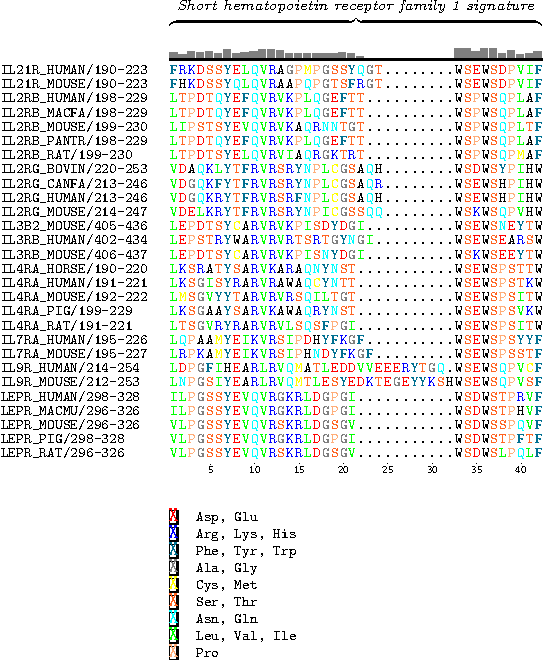
\includegraphics[width=0.80\textwidth]{Body/Images-chap1/hematopo.pdf}
            \caption[Regular grammar describing the short hematopoietin receptor family 1 signature]{
            Regular grammar describing the short hematopoietin receptor family 1 signature~\cite{hofmann1999prosite}.
            These proteins are mostly receptors for interleukin
            cytokines.  They are selectively expressed in lymphoid
            tissues and are typically membrane--bound~\cite{parrish-novak2000interleukin}.  The
            region shown in the figure is characterized by the
            regular expression
            \texttt{[LIVF].........[LIV][RK].(9,20)WS.WS....[FYW]}.
            This motif is required for
            proper protein folding, efficient intracellular transport, and cell--surface receptor
            binding.  The motif is relatively sensitive for the
            receptor family; however, it misses the rodent thymic stromal lymphopoietin protein
            receptors, which are in the same family.  Furthermore,
            the motif is not as specific as it could be --- as shown
            above, the motif matches five receptors for the leptin
            obesity factor, which are not in the same family.
            Notice that the bar at the top shows the degree of
            conservation at each position; the amino acids are
            colored to reflect their physiochemical properties; and,
            the bracketed expressions, such as \texttt{[LIV]}, tend
            to group together amino acids with similar physiochemical properties.
            }
            \label{fig:hemato}
            \end{figure}

Because it is a more compact representation, regular grammars are
usually recorded in regular expression form.  In contrast, more
complex grammars cannot be represented as a simple series of
characters and symbols.  This ease with which they can be
communicated has been one of the factors promoting the widespread
use of regular expressions --- it would be inconvenient to discover
a new protein motif and not be able to record the motif in an easily
interpretable form for publication.

The regular expression formalisms presented here, such as the
bracketed expression and the wild--card, are not exhaustive.  There
are many more terms that increase the richness of regular
expressions, such as the Kleene star, ``\texttt{*}'', which means
``zero or more of the preceding expression'' and the ``\texttt{+}''
symbol, which means ``one or more of the preceding expression.'' For
an exhaustive treatment of regular expressions, the reader is
referred is referred to publications
by~\citet{sipser1997introduction} and~\citet{friedl1997mastering}.

\subsubsection*{Matching regular grammars and regular expressions}

Thus far, I have described how regular expressions be used
to model a set of motif instances.  However, a very common task is
to then use a regular expression to look through new, longer
sequences for ``matches,'' i.e.\ subsequences of a given sequence
that are derivations of the grammar that the regular expression
encodes.  For example, consider the following regular expression:
\texttt{A[KR].Q[LV]C}.  We would like to know if there are any
derivations of this grammar within the sequence shown below.
\begin{equation}\label{eqn:randseq}
    \texttt{FLGARRQLCVVFKLAAKFQVCSKAKWQLCVFPAVFGKV}
\end{equation}
A simpleminded approach to this problem is to start with a beginning
of the sequence, at letter \texttt{F}, and ask whether or not a
derivation of the grammar could start that position.  Obviously, any
derivation of the grammar must begin with an \texttt{A}, so the
answer is ``no.''  Moving on to the first \texttt{A} in the
sequence, we see that it is followed by a \texttt{K}, which is
allowed by the grammar, and that the \texttt{K} can be followed by
any character, etc. Following this procedure reveals three matches
of the regular expression in the sequence, which are underlined
below.
\begin{equation}\label{eqn:randseq2}
    \texttt{FLG\uline{ARRQLC}VVFKLA\uline{AKFQVC}SK\uline{AKWQLC}VFPAVFGKV}
\end{equation}

In general, algorithms designed to match regular expressions against
sequences or other kinds of text use an approach that is, at its
core, the same as the simpleminded approach above.  One such
algorithm and piece of software is described in
Section~\vref{section:biogrep}.


\subsection*{Position weight matrices}\label{section:pwms}
\subsubsection*{Building position weight matrices}

    Despite their utility, regular grammars and regular expressions
    are not suitable for modeling all kinds of motifs.  As I showed
    earlier, regular grammars cannot describe long--range, nested,
    or crossing dependencies between characters.  However, there are
    also motifs where these dependencies do not exist and yet regular
    expressions are not accurate models.

    Consider the collection
    sequences shown in Figure~\vref{fig:yeast}.  This collection
    comprises numerous 3' splice sites from the fission yeast \emph{Schizosaccharomyces
    pombe}.  Each sequence is seven nucleotides in length and
    straddles the intron/exon boundary in a gene.  After
    transcription, these sites will form a ``branch point''
    allowing the introns to be excised from the pre--RNA to form the
    mature mRNA\@.

    Notice that to sensitively describe these sequences using a
    regular expression, we would use
    \texttt{[ATGC][ATGC][CT]T[ATG]A[CT]}.  This motif will match all
    of the instances, but it could also match many more: based on
    the number of bracketed expressions, this regular expression
    would match 192 unique sequences.

    Notice too that each column of the aligned instances shown
    in Figure~\ref{fig:yeast} has a particular ``preference'' for
    one kind nucleotide.  For example, all but 10 of the sequences
    have a thymine at the last position.  But, in the motif
    \texttt{[ATGC][ATGC][CT]T[ATG]A[CT]}, either cytosine or thymine
    is allowed in the last position, without any
    preference.  Obviously, this regular expression would be more
    specific if we labeled the last bracketed expression with these
    preferences, i.e. ``either cytosine or thymine, but with a
    seven--fold preference for the thymine.''


            \begin{sidewaysfigure}[ptb]
            \centering
            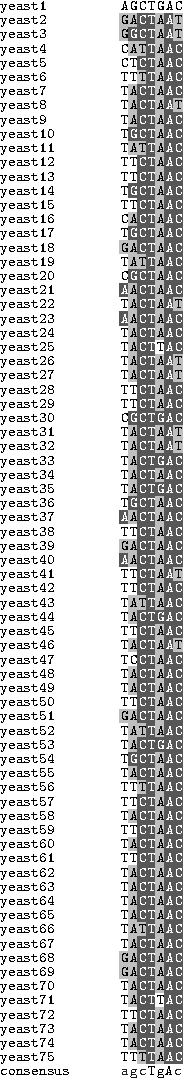
\includegraphics[angle=90]{Body/Images-chap1/yeast.pdf}
            \caption[Yeast 3' splice sites]{Yeast 3' splice sites.  The figure shows the 3'
             splice junction of 75 introns from the fission yeast \emph{Schizosaccharomyces pombe}.
             The coloring of the sequences is used to show the
             degree of conservation.  Notice that certain columns,
             such as the final column, have strong preferences for
             certain nucleotides.  The final column has a strong
             preference for cytosine; however, thymine is allowed
             occasionally.  The consensus sequence at the bottom
             shows the most common nucleotide at each position.  If
             the nucleotide is not perfectly conserved it is shown in
             lowercase.  This kind of motif is poorly modeled using
             regular grammars.  Instead, position weight matrices
             preserve much of the ``preference information.''
            }
            \label{fig:yeast}
            \end{sidewaysfigure}

    Incorporating such preferences into the grammatical framework
    requires only minor changes.  Recall from the definition on
    page~\pageref{gramDefs} that a grammar is
    regular (or right--linear or type--3) if each production in $P$ is of the form
    $A\rightarrow \texttt{x}B$, where $A$ and $B$ are in  $N$
    and $\texttt{x}$ is any string in $\Sigma*$.  A similar set
    of restrictions defines a position weight matrix, which is
    a grammar in which each production in $P$ is of the form
    $A\xrightarrow{p_i} \texttt{x}B$, where $A$ and $B$ are in  $N$
    and $\texttt{x}$ is any \textbf{character} in $\Sigma$,
    and $p_i$ is the probability of production $i$.  As well,
    $\sum_i p_1$ must equal one for all of the productions on which
    $A$ is on the left side.  In loose terms, the position weight
    matrix, or PWM, can be thought of as a probabilistic regular
    expression.  Using this new structure, the regular expression
    \texttt{[ATGC][ATGC][CT]T[ATG]A[CT]} can be written as a PWM
    grammar,
\begin{equation}\label{eqn:pwmGrammar}
    G = (\{S, \alpha, \beta, \gamma, \delta, \epsilon, \zeta, \eta\},\{\texttt{A}, \texttt{T},\texttt{G},\texttt{C}\},P,S),
\end{equation}
where $P$ is the set of productions below.
\begin{align}\label{eqn:pwmProduction}
    P =
    \begin{cases}
    S \rightarrow \alpha \\
    \alpha \xrightarrow{0.067} \texttt{A}\beta \\
    \alpha \xrightarrow{0.773} \texttt{T}\beta \\
    \alpha \xrightarrow{0.093} \texttt{G}\beta \\
    \alpha \xrightarrow{0.067} \texttt{C}\beta \\
    \beta \xrightarrow{0.627} \texttt{A}\gamma \\
    \beta \xrightarrow{0.240} \texttt{T}\gamma \\
    \beta \xrightarrow{0.120} \texttt{G}\gamma \\
    \beta \xrightarrow{0.013} \texttt{C}\gamma \\
    \gamma \xrightarrow{0.120} \texttt{T}\delta \\
    \gamma \xrightarrow{0.880} \texttt{C}\delta \\
    \delta \xrightarrow{1.000} \texttt{T}\epsilon \\
    \epsilon \xrightarrow{0.893} \texttt{A}\zeta \\
    \epsilon \xrightarrow{0.027} \texttt{T}\zeta \\
    \epsilon \xrightarrow{0.080} \texttt{G}\zeta \\
    \zeta \xrightarrow{1.000} \texttt{A}\eta \\
    \eta \xrightarrow{0.133} \texttt{T} \\
    \eta \xrightarrow{0.867} \texttt{C}
    \end{cases}
\end{align}
    Equation~\ref{eqn:hairpinProduction} can be represented much
    more compactly as a frequency matrix
    \begin{equation}\label{eqn:freq}
    f=
        \begin{pmatrix}
0.067 & 0.627 & 0.000 & 0.000 & 0.893 & 1.000 & 0.000 \\
0.773 & 0.240 & 0.120 & 1.000 & 0.027 & 0.000 & 0.133 \\
0.093 & 0.120 & 0.000 & 0.000 & 0.080 & 0.000 & 0.000 \\
0.067 & 0.013 & 0.880 & 0.000 & 0.000 & 0.000 & 0.867
        \end{pmatrix}
    \end{equation}
    in which each row corresponds to a single character in
    $\Sigma$ and each column corresponds to a single non--terminal
    character in  $N$ (where $\Sigma$ is disjoint from $N$, as
    usual).  So, in Equation~\ref{eqn:freq}, the rows correspond to
    \texttt{A}, \texttt{T}, \texttt{G}, and \texttt{C}; and the columns
    correspond to $\alpha$, $\beta$, $\gamma$, $\delta$, $\epsilon$, $\zeta$, and
    $\eta$, where $S$ was omitted.

    Notice that a derivation of the grammar in Equation~\vref{eqn:pwmGrammar}
    is necessarily also a derivation of the regular grammar
    \texttt{[ATGC][ATGC][CT]T[ATG]A[CT]}, and vice versa.  As such, the two grammars
    describe the same language, or the set of all derivations.  But,
    because the productions of Equation~\ref{eqn:pwmGrammar} are
    weighted by probability, certain derivations are more probable
    than others.  The degree to which one derivation of the grammar
    is more probable than another is characterized by the
    derivation's log--odds score.  To compute the log--odds score,
    first requires a log--odds matrix, $\Theta$, where
\begin{equation}\label{eqn:theta}
    \Theta_{ij} = \log_2 \left(\frac{f_{ij}}{q_j}\right).
\end{equation}

    The calculation of the frequency and log--odds matrices for the
    3' yeast splice sites is shown in Table~\ref{table:pwm}.  Here,
    $\Theta$ is given by
    \begin{equation}\label{eqn: theta2}
    \Theta =
        \begin{pmatrix}
-1.907 & 1.326 & \varnothing & \varnothing & 1.837 & 2.000 & \varnothing \\
1.629 & -0.059 & -1.059 & 2.000 & -3.229 & \varnothing & -0.907 \\
-1.421 & -1.059 & \varnothing & \varnothing & -1.644 & \varnothing & \varnothing \\
-1.907 & -4.229 & 1.816 & \varnothing & \varnothing &
\varnothing & 1.794
        \end{pmatrix},
    \end{equation}
    where $\varnothing$ is used to indicate values that are
    undefined because $f_{ij}=0$ and $\log_2 0$ is undefined.
    Given
    the log--odds matrix form of a PWM, the score of any derivation
    of the PWM is computed merely by looking up values in $\Theta$.
    Consider the sequence \texttt{AGCTGAC}, which is both a
    derivation of the grammar shown in Equation~\vref{eqn:pwmGrammar}
    and the first of the sequences shown in Figure~\vref{fig:yeast}.
    The log--odds score for this sequence is
    \begin{equation}\label{eqn:score}
        \begin{split}
          \text{score} &= \Theta_{0,0} + \Theta_{2,1}+ \Theta_{3,2}
                    + \Theta_{1,3}+ \Theta_{2,4}+ \Theta_{0,5}+ \Theta_{3,6}\\
            =& -1.907 -0.059 +1.816 +2.000 -1.644 +2.000 +1.794\\
            =& 4.000.
        \end{split}
    \end{equation}
    Notice that the score for a sequence that is not a derivation of
    the grammar is undefined, or, effectively $-\infty$.
    Table~\vref{table:pwm} shows the calculation of the frequency
    matrix, log--odds matrix, and the scoring of example sequences
    for this PWM\@.  Also, a small program for calculating a
    PWM from a set of sequences is provided in
    Section~\vref{section:pwmCode} of the Appendix.


        \newcolumntype{H}{>{\columncolor[gray]{0.8}}c}

\begin{table}[ptbh]
    \caption[The construction of a position weight matrix]{
        The construction of a position weight matrix from
        the collection of sequences shown in
        Figure~\vref{fig:yeast}.  Part A) shows the number of
        nucleotides of each type that occur in each of the seven
        positions of the aligned sequences.  For example, in the
        first position, there are 58 thymines.  Part B) shows the
        frequency matrix $f$, where each $f_{ij}=(c_{ij}/\sum_j
        c_{ij})$.  Part C) shows the log--odds matrix $\Theta$,
        where each $\Theta_{ij} =  \log_2 (f_{ij}/q_j)$
        and $q$ is the vector of background frequencies for the
        nucleotides.  Part D) shows the scoring of three different
        sequences.  To compute the score for a sequence, the
        corresponding nucleotide at each column is looked up in
        $\Theta$ and the columns are summed together.
        }
            \label{table:pwm}
                    \centering \scriptsize
            \begin{tabular}{r|HcHcHcH} %\hline\hline
\multicolumn{8}{l}{} \\
\multicolumn{8}{l}{A) Count  Matrix ($c_{ij}$):} \\
\multicolumn{8}{l}{} \\
A & 5 & 47 & 0 & 0 & 67 & 75 & 0 \\
T & 58 & 18 & 9 & 75 & 2 & 0 & 10 \\
G & 7 & 9 & 0 & 0 & 6 & 0 & 0 \\
C & 5 & 1 & 66 & 0 & 0 & 0 & 65 \\
  \multicolumn{4}{c}{ }& $\Downarrow$\\
\multicolumn{8}{l}{B) Frequency  Matrix ($f_{ij}$):} \\
\multicolumn{8}{l}{} \\
A & 0.067 & 0.627 & 0.000 & 0.000 & 0.893 & 1.000 & 0.000 \\
T & 0.773 & 0.240 & 0.120 & 1.000 & 0.027 & 0.000 & 0.133 \\
G & 0.093 & 0.120 & 0.000 & 0.000 & 0.080 & 0.000 & 0.000 \\
C & 0.067 & 0.013 & 0.880 & 0.000 & 0.000 & 0.000 & 0.867 \\
  \multicolumn{4}{c}{ }& $\Downarrow$\\
\multicolumn{8}{l}{C) Log--odds  Matrix ($\Theta_{ij}$):} \\
\multicolumn{8}{l}{} \\
A & -1.907 & 1.326 & $\varnothing$ & $\varnothing$ & 1.837 & 2.000 & $\varnothing$ \\
T & 1.629 & -0.059 & -1.059 & 2.000 & -3.229 & $\varnothing$ & -0.907 \\
G & -1.421 & -1.059 & $\varnothing$ & $\varnothing$ & -1.644 & $\varnothing$ & $\varnothing$ \\
C & -1.907 & -4.229 & 1.816 & $\varnothing$ & $\varnothing$ & $\varnothing$ & 1.794 \\
  \multicolumn{4}{c}{ }& $\Downarrow$\\
\multicolumn{8}{l}{D) Example sequence scoring:} \\
\multicolumn{8}{l}{} \\
query1 & T & A & C & T & T & A & C\\
$\Sigma$ & 1.629  & 1.326 & 1.816 & 2.000 & -3.229 & 2.000 & 1.794\\
  \multicolumn{4}{c}{ }& $= 7.335$\\
query2 & T & T & C & T & A & A & C \\
$\Sigma$ & 1.629  & -0.059 & 1.816 & 2.000 & 1.837 & 2.000 & 1.794\\
  \multicolumn{4}{c}{ }& $= 11.017$\\
query3 & G & T & A & T & A & A & T \\
$\Sigma$ & -1.421  & -0.059 & $\varnothing$ \\
  \multicolumn{4}{c}{ }& $= \varnothing$\\
%\hline\hline
\end{tabular}
\end{table}


    The ``strength'' of a PWM motif is measured by a quantity called
    its entropy.  The motif entropy is the sum of the entropies of
    each column, or position in the motif.
    This entropy of a given column in a PWM is a measure of the
    disorder, or the randomness of the distribution of letters.  The
    column entropy is measured in bits and is given by
        \begin{equation}\label{eqn:pwmh}
            h_i = -\sum_{j} f_{ij}\log_2 f_{ij}
        \end{equation}
    where, $f_{ij}$ is the frequency matrix as shown in
    Figure~\vref{table:pwm}.  The entropy of the whole motif
    is just the sum of the entropies of the columns:
        \begin{equation}\label{eqn:pwmH}
            H = -\sum_{i}\sum_{j} f_{ij}\log_2 f_{ij}.
        \end{equation}

    Typically, the entropy is measured
    relative to the background entropy.  As above, the background
    entropy of a single column is
        \begin{equation}\label{eqn:pwmbgh}
            h_i^\circ = -\sum_{j} q_{j}\log_2 q_{j}
        \end{equation}
    where, $q_{j}$ is the \emph{a priori}, background frequency of
    the letter denoted by index $j$.  In the case of identically
    distributed nucleotides, each $q_j$ is $0.25$; i.e.\ $q_A=0.25$,
    $q_C=0.25$, $q_T=0.25$, and $q_G=0.25$.  The background entropy
    of the entire motif is
        \begin{equation}\label{eqn:pwmbgH}
            H^{\circ} = -\sum_{i}\sum_{j} q_j\log_2 q_j.
        \end{equation}

    The difference between the background entropy and the motif
    entropy is referred to as the information content, $I$, of the PWM\@.
    Using Equations~\ref{eqn:pwmh}--~\ref{eqn:pwmbgH} above, the
    information content can be calculated as
        \begin{equation}\label{eqn:pwmI}
            \begin{split}
              I &=  H^{\circ}-H\\
                &= -\sum_{i}\sum_{j} q_j\log_2 q_j - \left(-\sum_{i}\sum_{j}f_{ij}\log_2 f_{ij}\right)\\
                &= \sum_{i}\sum_{j}f_{ij}\log_2
                \left(\frac{f_{ij}}{q_j}\right).
            \end{split}
        \end{equation}
    Notice that the information content of the motif is minimized
    when the nucleotide distribution for each column is exactly the
    background distribution of nucleotides.  That is, when $f_{ij}=q_j$
    for all $i$, the $\log_2(f_{ij}/q_j)$ terms are zero.
    This makes sense intuitively: if the PWM describes the
    background distribution, the motif can obviously not be
    distinguished from the background and therefore contains no
    information.  In this same case, the entropy of the motif is
    maximized and is equal to the background entropy.

    PWMs are commonly represented by two varieties of schematics:
    pictograms and sequence logos.  An example of each of these is
    shown in Figure~\vref{fig:yeastLogo}.
    A pictogram is essentially a visualization of the frequency
    matrix representing a PWM, whe, whereas  A sequence logo is a pictogram
    that is scaled to reflect the information content at each
    position in the PWM\@.

            \begin{figure}[ptb]
        A) Pictogram of the PWM in Table~\vref{table:pwm}
            \begin{center}
            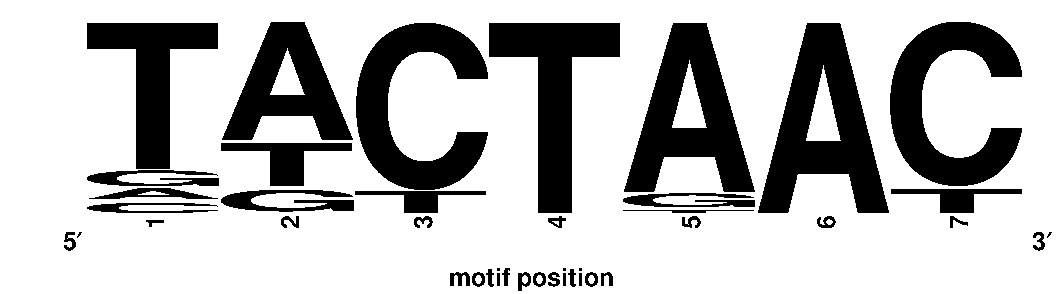
\includegraphics[width=\textwidth]{Body/Images-chap1/yeast-logo2.pdf}
            \end{center}
        \bigskip
            B) Logo of the PWM in Table~\vref{table:pwm}
            \begin{center}
        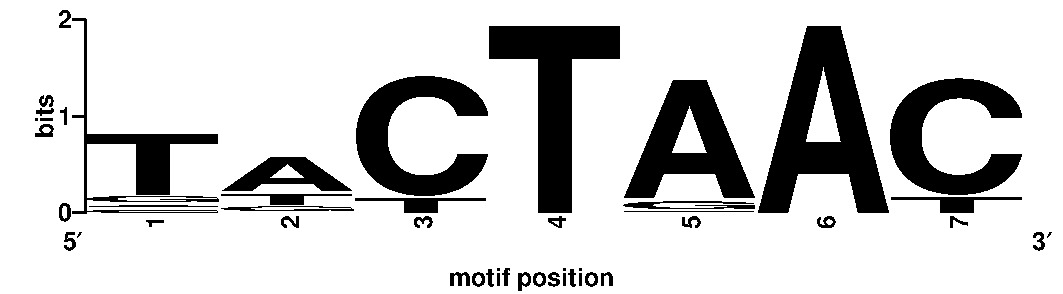
\includegraphics[width=\textwidth]{Body/Images-chap1/yeast-logo1.pdf}
            \end{center}
            \caption[Yeast 3' splice site pictogram and logo]{
            Yeast 3' splice site pictogram and logo. Part A) shows
            the
            PWM in Table~\vref{table:pwm} represented as a
            pictogram.  At each position in the motif, the height of
            the nucleotides is scaled in proportion to their
            frequency in $f$, with the more frequent nucleotides
            always placed on top.  The pictogram clearly shows that
            positions four and six are perfectly conserved, whereas
            the other positions are distributed between many
            nucleotides.  Part B) shows a sequence logo
            representation of the same PWM.  The sequence logo is a
            pictogram in which the height of each column is scaled
            in proportion to the information content contributed by
            that position to the motif (see
            Equation~\vref{eqn:pwmI}).  Taller columns have a
            nucleotide distribution that deviates strongly from the
            background distribution.  In this sequence logo, the
            background distribution is arbitrarily set to equal
            \emph{a priori} probability of each nucleotide.  As
            such, the maximum information content in any column is
            two bits, which is achieved only in the two perfectly
            conserved positions of the motif.
            }
            \label{fig:yeastLogo}
            \end{figure}

\subsubsection*{Matching position weight matrices}

        Thus far, I have shown how a PWM can be used to model a
        set of motif instances and how a derivation of a PWM
        grammar can be scored.  PWMs can also be used to search in
        new, long sequences for regions of the sequence that appear
        to match the motif.  This is accomplished by ``sliding'' the
        PWM over the length of the sequence to look for subsequences
        that have high log--odds scores.

        Consider searching the sequence \texttt{TAGCTGACTGAC}.  To
        slide the PWM over this sequence is equivalent to evaluating
        the score of each seven nucleotide substring:
        \texttt{TAGCTGA},
        \texttt{AGCTGAC},
        \texttt{GCTGACT},
        \texttt{CTGACTG},
        \texttt{TGACTGA}, and
        \texttt{GACTGAC}.  These are $\varnothing$, 4.0,
         $\varnothing$, $\varnothing$, $\varnothing$, and
         5.871.  That is, there are two matches for the PWM, one
         stronger than the other.  This method can be used to search
         for a PWM in much larger sequences as well.  For example,
         Figure~\ref{fig:pwmHits} (page~\pageref{fig:pwmHits}) shows the distribution of scores
         obtained by searching
            the PWM in Table~\vref{table:pwm} against chromosomes 1--4 of
        the
            \emph{Saccharomyces cerevisiae} genome.


            \begin{figure}[ptb]
            \centering
            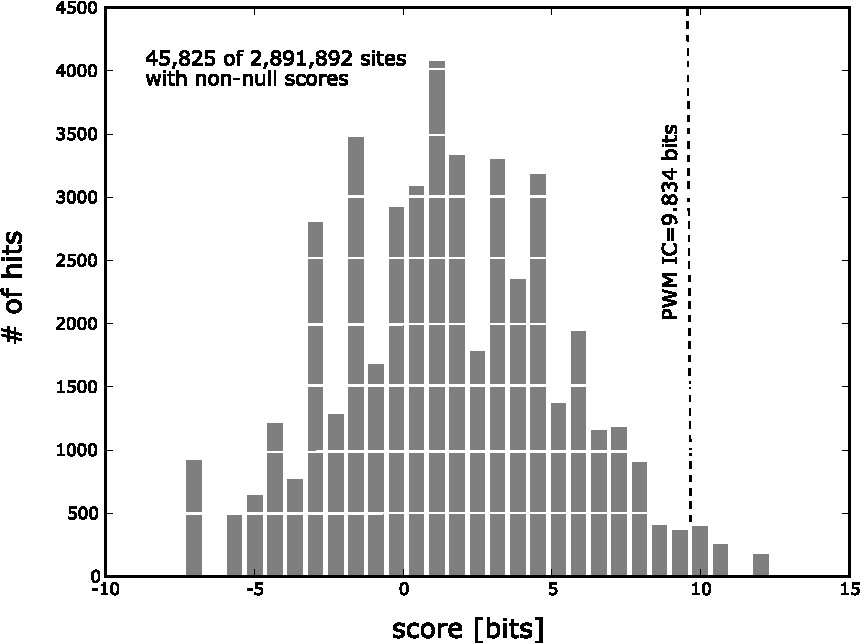
\includegraphics[width=\textwidth]{Body/Images-chap1/pwmHits.pdf}
            \caption[pwmHits]{Distribution of log--odds scores obtained by searching
            the PWM in Table~\vref{table:pwm} against chromosomes 1--4 of
            \emph{Saccharomyces cerevisiae}.  Of the nearly 3
            million possible sites, only 46,000 had non--null
            scores.  As the figure shows, the score distribution is
            roughly Gaussian.  The dashed line indicates the
            information content of the PWM\@.  Scores above this
            line are generally considered  strong matches.
            PWMs are more specific than regular grammars, because
            the threshold above which a match is considered ``true''
            can be varied.  In contrast, with a regular grammar is
            either a match or not a match: there is no variable threshold.
        }
            \label{fig:pwmHits}
            \end{figure}



\section{Tools for motif discovery}\label{section:tools}
\subsection*{Introduction}

    In general, the goal of motif discovery is to derive a set of
    grammars that sensitively matches a set of given sequences.
    This is the inverse of many of the examples in the previous
    section.  That is, imagine a case in which you are given a set
    of derivations and then asked what kind of grammar could have
    produced the derivations?  This is what is called grammar
    induction in  the computational linguistics literature and is
    equivalent to guessing the grammar of an unknown language given a few
    sentences in the language.

    In bioinformatics, this task is usually presented in a slightly
    more difficult form.  To illustrate this, consider a
    hypothetical challenge in which a colleague hides derivations of
    the regular grammar \texttt{[KR]QTRP.[RT]K} in a set of
    sequences that consist otherwise of random characters.  You are
    presented with the sequences and asked what grammar was hidden
    therein.
    \begin{equation}\label{eqn:hidden1}
        \begin{split}
          \texttt{AJDFIOASODVIKQTRPXYKIIWEJSJ} \\
          \texttt{JKQTRPCRKXUCIQWEMFIOAKLGS} \\
          \texttt{ADUHFIKACRQTRPXKMSKDAFIOAS}
        \end{split}
    \end{equation}
    Without any prior knowledge, this task is nearly impossible.
    The colleague could have hidden a regular grammar that consisted
    solely of \texttt{S}, which would be undetectable since there are many characters
    that occur in all of the sequences.  Further, he could have hidden ``\texttt{....}'',
    in which case there would be no evidence in the sequences.
    This conundrum is closely related to one of the three tenets
    of motif discovery
    developed in Section~\vref{section:tenents}: the answer to any
    motif discovery question is invariably dependent on at least
    some prior knowledge about what forms a motifs may take.

    Suppose then that the colleague says the motif is at least five
    characters long, is a regular grammar, and all the derivations
    of the grammar look ``pretty similar.''  Given this
    information, a logical approach would be to look for
    subsequences of five characters that look relatively similar and
    occur in all three sequences.  After diligently scanning the
    sequences, you can find two sets of three that seemed to fit
    this description: $\{\texttt{FIOAS}, \texttt{FIOAK},
    \texttt{FIOAS}\}$ and $\{\texttt{KQTRP}, \texttt{KQTRP},
    \texttt{RQTRP}\}$.  Knowing the answer, it is obvious that we
    are on the right track; however, again we are at an impasse.
    It would be easy to write a regular expression describing either
    of these sets.  But, \emph{a priori} it is impossible to tell
    which set may be the correct answer.  The first set has a \texttt{K}
    that is mismatched with a \texttt{S}, whereas the latter set has
    a \texttt{K}--\texttt{R} mismatch.  If these were amino acid
    sequences we could say that lysine, \texttt{K}, is more similar
    to arginine, \texttt{R}, than it is to serine, \texttt{S}.
    Therefore, we might choose the latter set.  This decision is
    related to the remaining two tenets of motif discovery developed
    in Section~\ref{section:tenents}: the answer to any motif
    discovery problem will always depend on a predefined metric of
    similarity and a method for grouping together similar objects.


    In the following sections, I review a number of approaches for
    problems such as the example given above,
    focusing on the two most common classes of
    approach: those that use regular expression motif models and
    those that use PWMs.  All of these approaches, without
    exception, always require some degree of intelligent guidance by
    the user that can be reduced to the three tenets discussed
    above.  In general, motif discovery tools that do not have such
    requirements have made assumptions on the user's behalf.



\subsection*{Teiresias and other regular expression--based
tools}\label{section:teiresias}

    Because they are convenient from both a computational
    perspective and from the perspective of communicating results,
    regular expressions are the most common form of motif model used
    in bioinformatics.  Table~\vref{table:regexMD} shows a list of
    publications introducing motif discovery tools in this class.
    Within the field, these algorithms are commonly referred to as ``motif driven''
    or ``pattern driven''
            algorithms~\cite{brazma1998pattern}.
            At their most basic conceptual level, all of these
            approaches work by first enumerating possible patterns
            and then checking for the patterns in the sequence
            set~\cite{brazma1998pattern}.

            There are three principal characteristics that distinguish between the various
            algorithms shown in Table~\ref{table:regexMD}, which are as
            follows:
            \begin{enumerate}
                \item   The regular expression class complexity.
                \item   The completeness of the returned motif set.  That is, does the algorithm return \emph{all}
                        patterns present in the input sequences?
                \item   The motif \emph{maximality}.  For instance, in the two strings ``\texttt{KYLEJ}'' and ``\texttt{KYLEL}'',
                        the motif ``\texttt{KYLE}'' is maximal, whereas ``\texttt{KYL}'' is not, because we could
                        add an ``\texttt{E}'' without decreasing the number of times it
                        occurs.  In essence, maximality is a proxy
                        for specificity.
            \end{enumerate}

        \begin{table}[ptbh]
    \caption[Motif discovery tools using regular expressions or similar models]{
        Motif discovery tools using regular expressions or similar
        models.  This list is not intended to be exhaustive;
        however, it includes many of the well--known motif discovery
        tools used in bioinformatics.  Early methods tended to use
        consensus strings or simple word counting approaches, i.e.\
        counting the occurrences of ``n--mers'' such as the 4--mer
        \texttt{ATGC}.  Words that are statistically over--represented
        are called motifs.  Later approaches used more complex
        regular expressions, cf.~\citet{rigoutsos1998combinatorial}.
        }
            \label{table:regexMD}
                    \centering
            \begin{tabular}{lcc} \hline\hline
Authors & Year & Citation \\ \hline
\citeauthor{queen1982improvements} & \citeyear{queen1982improvements} & \cite{queen1982improvements} \\
\citeauthor{galas1985rigorous} & \citeyear{galas1985rigorous} & \cite{galas1985rigorous} \\
\citeauthor{mengeritsky1987recognition} & \citeyear{mengeritsky1987recognition} & \cite{mengeritsky1987recognition} \\
\citeauthor{staden1989methods} & \citeyear{staden1989methods} & \cite{staden1989methods} \\
\citeauthor{neuwald1994detecting} & \citeyear{neuwald1994detecting} & \cite{neuwald1994detecting} \\
\citeauthor{jonassen1995finding} & \citeyear{jonassen1995finding} & \cite{jonassen1995finding} \\
\citeauthor{wolferstetter1996identification} & \citeyear{wolferstetter1996identification} & \cite{wolferstetter1996identification} \\
\citeauthor{sagot1997multiple} & \citeyear{sagot1997multiple} & \cite{sagot1997multiple} \\
\citeauthor{rigoutsos1998combinatorial} & \citeyear{rigoutsos1998combinatorial} & \cite{rigoutsos1998combinatorial,floratos1999pattern} \\
\citeauthor{van1998extracting} & \citeyear{van1998extracting} & \cite{van1998extracting,van2000discovering} \\
\citeauthor{jacobs2000computational} & \citeyear{jacobs2000computational} & \cite{jacobs2000computational} \\
\citeauthor{marsan2000algorithms} & \citeyear{marsan2000algorithms} & \cite{marsan2000algorithms} \\
\citeauthor{pevzner2000combinatorial} & \citeyear{pevzner2000combinatorial} & \cite{pevzner2000combinatorial} \\
\citeauthor{bussemaker2000building} & \citeyear{bussemaker2000building} & \cite{bussemaker2000building} \\
\citeauthor{kielbasa2001combining} & \citeyear{kielbasa2001combining} & \cite{kielbasa2001combining} \\
\citeauthor{horton2001tsukuba} & \citeyear{horton2001tsukuba} & \cite{horton2001tsukuba} \\
\citeauthor{keich2002subtle} & \citeyear{keich2002subtle} & \cite{keich2002subtle} \\
\citeauthor{eskin2002finding} & \citeyear{eskin2002finding} & \cite{eskin2002finding} \\
\citeauthor{buhler2002finding} & \citeyear{buhler2002finding} & \cite{buhler2002finding} \\
\citeauthor{sinha2002discovery} & \citeyear{sinha2002discovery} & \cite{sinha2002discovery} \\
\citeauthor{price2003finding} & \citeyear{price2003finding} & \cite{price2003finding} \\
\citeauthor{sinha2003discriminative} & \citeyear{sinha2003discriminative} & \cite{sinha2003discriminative} \\
\citeauthor{danilova2003an} & \citeyear{danilova2003an} & \cite{danilova2003an} \\
\citeauthor{ganesh2003mopac} & \citeyear{ganesh2003mopac} & \cite{ganesh2003mopac} \\
\citeauthor{liang2004cwinnower} & \citeyear{liang2004cwinnower} & \cite{liang2004cwinnower} \\
\citeauthor{fogel2004discovery} & \citeyear{fogel2004discovery} & \cite{fogel2004discovery} \\
\citeauthor{pavesi2004weeder} & \citeyear{pavesi2004weeder} & \cite{pavesi2004weeder} \\
\citeauthor{hernandez2004model} & \citeyear{hernandez2004model} & \cite{hernandez2004model} \\
\citeauthor{markstein2004regulatory} & \citeyear{markstein2004regulatory} & \cite{markstein2004regulatory} \\
\citeauthor{frith2004finding} & \citeyear{frith2004finding} & \cite{frith2004finding} \\
\citeauthor{sumazin2005dwe} & \citeyear{sumazin2005dwe} & \cite{sumazin2005dwe} \\
\hline
\end{tabular}
\end{table}


            The most important of these distinguishing features
            is the complexity of the regular expression class that
            an algorithm returns.  No motif discovery tool can
            search for the ``universe'' of regular expressions.
            Recall from the previous section that ``\texttt{...}''
            and other types of motifs will always be present, and
            therefore such a result is meaningless.  Furthermore,
            enumerating regular expressions is
            NP--complete~\cite{maier1978complexity,garey1979computers},
            meaning that, in general, the runtime of a motif
            discovery tool will increase exponentially with the size
            of the sequence set it is given.  As I showed in the
            previous section, the answer to any motif discovery
            problem will always require some \emph{a priori}
            knowledge of the kinds of motifs that might be found, and
            simply specifying that the grammar is regular is not
            enough.  Accordingly, most motif discovery tools
            restrict themselves to finding a particular subclass of
            regular expressions.
            This motif class determines the form of each
            pattern, $p_i$ that we find.  Below, a few motif classes, commonly
            used in biological sequence analysis,  are enumerated in
            order of increasing complexity~\cite{floratos1999pattern}:

            \begin{itemize}
                \item   $p_i\in\Sigma^{\ast}$:  This is the class
                        of all ``solid'' patterns, for example
                        ``\texttt{KAGTPT}'' and ``\texttt{TAGCGGGAT}''.

                \item   $p_i\in(\Sigma\cup\{.\})^{\ast}$:  This is the
                        class of all patterns that can have ``wildcard''
                        positions, which are denoted by ``.'', for example
                        ``\texttt{K.G.PT}'' and ``\texttt{TA...GGAT}''.
                        The wildcard means that any character from the
                        alphabet will suffice in that position.

                \item   $p_i\in(\Sigma\cup R)^{\ast}$: This
                        is the class of all patterns that can
                        have ``bracketed'' expressions, for
                        example ``\texttt{K[ADG]G[KQ]PT}'' and
                        ``\texttt{TA[GA][TC]GGAT}''.  The bracketed
                        expression ``[\texttt{TC}]'' means that either
                        ``\texttt{T}'' or ``\texttt{C}'' will suffice in
                        that position.  In this notation, $R$ represents
                        the set of characters in the brackets, for example
                        $R=\{\texttt{TC}\}$ or $R=\{\texttt{GA}\}$.

                \item   $p_i\in(\Sigma\cup .)^{\ast}$:  This is the
                        class of ``flexible'' patterns.  For example
                        ``\texttt{K.(1,3)G.(2,5)PT}'', where ``.(2,5)''
                        means that anywhere between two and five wildcards
                        can exist at that position, that is .(2,5)
                        can be any one of $\{..,...,....,......\}$.

            \end{itemize}
            In general, the more complex these patterns are, the more expressive the languages will be that we find.  However,
            with increasing complexity, the computational difficulty of the motif discovery problem increases
            drastically~\cite{maier1978complexity,garey1979computers}.



            Also, for some of these tools, it is possible to
            guarantee the completeness of the set of returned
            patterns.  That is, a particular tool may guarantee that all
            regular expressions meeting particular characteristics are discovered.
            However, this guarantee comes at the price of
            increased time and space complexity.  That is, the set
            of all possible patterns is very large and can take a
            large space to enumerate and a long time to search
            through.  As such, many motif driven algorithms
            use heuristics to limit the space of patterns that are
            searched.

            Here, I will focus on the Teiresias algorithm as a representative
            regular expression--based motif discovery tool.
            Notably, Teiresias is the basis for much of the work in
            this thesis, particularly in Chapters 1 and 2.
            A more detailed description of Teiresias is available elsewhere~\cite{floratos1999pattern,rigoutsos1998combinatorial}.


            Given a set of sequences $S = \{ s_0,s_1,\ldots,s_n\}$,
            and integers $L$, $W$, and $K$, Teiresias finds all
            patterns involving at least $L$ non--wildcard characters
            that occur at least $K$ times and have a fraction of
            non--wildcard characters of at least $L/W$.  This set of
            patterns is called $\mathcal{C}$, where $\mathcal{C}=\{
            p_1,p_2,\ldots,p_m\}$ and each $p_i\in\teirRegEx$.
            This is the set of all regular expressions that begin
            and end with a character, but may have an arbitrary
            number of wild--cards and characters in the middle
            subject to the $L$ and $W$ restriction,
            for example, \texttt{AXG}, \texttt{A.G},
            \texttt{K..R.G}, etc.
            For
            each motif $p_i$ in $\mathcal{C}$, Teiresias returns an
            offset list $\mathscr{L}\paren{p_i}$ that specifies each
            sequence--position combination where the motif occurs
            (cf.\ Figure~\vref{fig:teiresias output}).

            The support of a motif is equal to
            the number of its occurrences (or, equivalently, ``instances'' or ``embeddings''),
            $\vert \mathscr{L}(p) \vert$.
            Essentially,
            $L$ defines the minimum size of patterns in which we are
            interested, and $L/W$ defines the minimum specificity
            (the fewer wildcards, the more specific a motif).
            The four distinguishing characteristics of the Teiresias algorithm are as follows:
            \begin{enumerate}
                \item   All \emph{maximal} patterns are reported (see below for a definition of ``maximal'').
                \item   Only the maximal patterns are reported.
                \item   Running time depends only on the number of patterns present in
                        the data, that is it is \emph{output sensitive}.
                \item   Patterns can be arbitrarily long.
            \end{enumerate}
            The most important characteristic of Teiresias is that it returns the \emph{complete} set of maximal patterns.
            And, because of the manner in which these patterns are handled internally by Teiresias, the algorithm runs
            very quickly.

    In the Teiresias parlance, a maximal motif is a regular expression which has the following properties:
        \begin{enumerate}
        \item   The motif cannot be made more specific
            without producing a motif with
            fewer embeddings (i.e., without
            $\vert \mathscr{L}(p) \vert$
            decreasing); and

        \item   The motif is not missing any instances,
            i.e.\ $\mathscr{L}(p)$ includes the locations
            of all instances of the motif.

        \end{enumerate}
    These two criteria can be summarized qualitatively by stating that a maximal
    motif is not ``missing'' any locations and is as wide as possible, and
    thus it is as specific and sensitive as possible.  Here,
    ``specific'' has a particular meaning: a pattern $p_i$ is more
    specific than $p_j$ if $p_j$ can be transformed into $p_i$ by
    substituting one or more wild--cards for a character, or by
    appending wild--cards and characters to either side of $p_j$.
    For example, \texttt{CH.MEN..N} is less specific than all of the
    following regular expressions: \texttt{CHEMEN..N},
    \texttt{CH.MEN..NE.R},
    and \texttt{CH.MEN.IN}.
    Necessarily, if a pattern $p_i$ is more specific than a pattern $p_j$, then
    \begin{equation}\label{eqn:support}
        \vert \mathscr{L}(p_i) \vert \leq
        \vert \mathscr{L}(p_j) \vert .
    \end{equation}

    Teiresias works in two phases: scanning and convolution.
    During the scanning phase, Teiresias enumerates
    all ``elementary motifs'' with exactly $L$ characters and at most $W-L$
    wild--cards (see Figure~\vref{fig:teiresiasExample}).
    Elementary motifs are short regular expressions that can be
    stitched together to form longer regular expressions that are
    more specific, using the definition of specificity above.  For
    example, as shown in Figure~\ref{fig:teiresiasExample}, the
    sequences
    \begin{equation*}
        \begin{split}
          \texttt{KDWVQKRK} \\
          \texttt{CWCQKRK} \\
          \texttt{WDQKRKNP}
        \end{split}
    \end{equation*}
    have five motifs with 1) exactly $L=3$ characters, 2) no more than
    $W-L$ wild--cards for every window of $L=3$ characters,
    and that 3) occur at least three times:
    \texttt{W.QK}, \texttt{QKR}, \texttt{QK.K}, \texttt{KRK},
    and \texttt{Q.RK}.  These are the elementary motifs.

           \begin{figure}[ptb]
            \centering
\begin{verbatim}
                           >seq 0
                           KDWVQKRK
                           >seq 1
                           CWCQKRK
                           >seq 2
                           WDQKRKNP
\end{verbatim}

            $\Downarrow$\\
    Teiresias\\
    $L/W/K = 3/4/3$ \\
            $\Downarrow$\\

            Elementary motifs: \\

            \begin{tabular}{lccccc} \hline\hline
            motifs $\rightarrow$ & \texttt{W.QK~~} & \texttt{~~QKR}& \texttt{~~QK.K}& \texttt{~~~KRK}&
            \texttt{~Q.RK}\\ \hline
            \multirow{2}{*}{offset \#0} &
            \texttt{KD\textbf{W}V\textbf{QK}RK~~} &
            \texttt{KDWV\textbf{QKR}K~~} &
            \texttt{KDWV\textbf{QK}R\textbf{K}~~} &
            \texttt{KDWVQ\textbf{KRK}~~} &
            \texttt{KDWV\textbf{Q}K\textbf{RK}~~} \\
            & (0,2)
            & (0,4)
            & (0,4)
            & (0,5)
            & (0,4)\\ \hline
            \multirow{2}{*}{offset \#1} &
            \texttt{~C\textbf{W}C\textbf{QK}RK~~} &
            \texttt{~CWC\textbf{QKR}K~~} &
            \texttt{~CWC\textbf{QK}R\textbf{K}~~} &
            \texttt{~CWCQ\textbf{KRK}~~} &
            \texttt{~CWC\textbf{Q}K\textbf{RK}~~} \\
            & (1,1)
            & (1,3)
            & (1,3)
            & (1,4)
            & (1,3) \\ \hline
            \multirow{2}{*}{offset \#2} &
            \texttt{~~\textbf{W}D\textbf{QK}RKNP} &
            \texttt{~~WD\textbf{QKR}KNP} &
            \texttt{~~WD\textbf{QK}R\textbf{K}NP} &
            \texttt{~~WDQ\textbf{KRK}NP} &
            \texttt{~~WD\textbf{Q}K\textbf{RK}NP} \\
            & (2,0)
            & (2,2)
            & (2,2)
            & (2,3)
            & (2,2) \\ \hline\hline
            \end{tabular}
            \caption[Scanning phase of Teiresias]{
            Scanning phase of Teiresias.  During the scanning phase, Teiresias enumerates
            all elementary motifs with exactly $L$ characters and at most $W-L$ wild--cards.
            Using the input sequences above, Teiresias finds five such elementary motifs
            as shown in the table: \texttt{F.AS}, \texttt{AST}, \texttt{AS.S}, \texttt{STS}, and
            \texttt{A.TS}.  The offset list for each of these is shown in the table.
            In the next phase of the algorithm, these elementary motifs are convolved
            together to form the final, maximal motifs.}
            \label{fig:teiresiasExample}
            \end{figure}

            In the convolution phase, the elementary motifs are
            stitched together to see if more specific motifs can be
            found.  The process of convolution is defined as
            follows:
    \begin{equation}\label{eqn:convolution}
    \begin{split}
        p_k &= p_i \oplus p_j\\
        & =
        \begin{cases}
        p_k p_i' & \text{if $\suffix_L(p_i)=\prefix_L(p_j)$,}\\
        \varnothing & \text{otherwise.}
        \end{cases}
    \end{split}
    \end{equation}
    In the equation above $\prefix_L(p_i)$ is  the sub--pattern
    at the beginning of
    $p_i$ with exactly $(L-1)$ characters.  Similarly, $\suffix_L(p_i)$ is  the sub--pattern
    at the end of
    $p_i$ with exactly $(L-1)$ characters.  For example:
    \begin{equation}\label{eqn:prefixsuffix}
        \begin{split}
          \prefix_3(\texttt{W.QK}) & = \texttt{W.Q} \\
          \suffix_3(\texttt{W.QK}) & = \texttt{QK} \\
          \prefix_3(\texttt{QKR}) & = \texttt{QK} \\
          \suffix_3(\texttt{QKR}) & = \texttt{KR}~.
        \end{split}
    \end{equation}
    To illustrate this, consider the following examples:
    \begin{equation*}
    \begin{split}
        \texttt{DF.A.T}\oplus\texttt{A.TSE}&=\texttt{DF.A.TE}\\
        \texttt{L.XF.A.MM}\oplus\texttt{A.MSE}&=\texttt{L.XF.A.MME}\\
        \texttt{WX.N.N}\oplus\texttt{N.PSE}&=\varnothing.
    \end{split}
    \end{equation*}

    If two motifs can be convolved --- i.e.\ $p_i \oplus
    p_j\neq\varnothing$ --- then the offsets of the new,
    longer regular expression, $p_k$ are given by
    \begin{equation}\label{eqn:offsetSize}
        \mathscr{L}(p_k) = \left\{(x,y) \in \mathscr{L}(p_i) \vert
            ~\exists(x,z)\in\mathscr{L}(p_j) \text{~such that~}
            z-y=\mathscr{W}(p)-\mathscr{W}(\suffix_L(p))\right\}.
    \end{equation}
    If $\vert \mathscr{L}(p_k) \vert < K$ then the motif does not
    have sufficient support and is discarded.  Conversely,
    if $\vert \mathscr{L}(p_k) \vert = \vert \mathscr{L}(p_i) \vert$
    then $p_i$ is not a maximal motif.  Or if $\vert \mathscr{L}(p_k) \vert = \vert \mathscr{L}(p_j) \vert$
    then $p_j$ is not a maximal motif.  But, if
    \begin{equation}\label{eqn:conv4}
            \vert p_i \oplus p_j \vert < K\text{~}\forall\text{~}j,
    \end{equation}
    then $p_i$ is maximal.


    Obviously, by convolving each elementary motif with every other
    elementary motif,
    i.e. by repeating $p_k = p_i \oplus p_j$ for all $i$ and $j$,
    the maximal motifs can be discovered.
    Teiresias uses an intelligent method of sorting the elementary
    motifs that does not require doing the all--by--all comparison
    and yet still guarantees that all the maximal motifs are
    discovered.  The set of these maximal motifs are then returned
    to the user as in Figure~\vref{fig:teiresias output}.


            \begin{figure}[ptb]
\begin{verbatim}
    >sequence 0
    MSKNIVLLPGDHVGPEVVAEAVKVLEAVSSAIGVKFNFSKHLIGGASIDAYGVPLSDEALEAAKK
    >sequence 1
    MSKQILVLPGDGIGPEIMAEAVKVLELANDRFQLGFELAEDVIGGAAIDKHGVP
    >sequence 2
    MKFLILLFNILCLFPVLAADNHGVGPQGASGVDPITFDINSNQTGPAFLT
\end{verbatim}

            \centering
            $\Downarrow$\\
    Teiresias:\\
    $L/W/K = 5/8/2$ \\
            $\Downarrow$\\

            Final motifs:\\

            \begin{tabular}{cccc} \hline\hline
            % after \\ : \hline or \cline{col1-col2} \cline{col3-col4} ...
            motif & \multicolumn{2}{c}{location (seq,pos)} \\ \hline
            \ttfamily GPE..AEAVKVLE & (0,13) & (1,13) \\
            \ttfamily IGGA.ID..GVP & (0,42) & (1,42) \\
            \ttfamily MSK.I..LPGD..GPE & (0,0) & (1,0) \\
            \ttfamily A.D.HGV & (1,46) & (2,17)\\ \hline\hline
            \end{tabular}
            \caption[Pattern discovery with Teiresias]{Pattern discovery with Teiresias.  Here we have three protein
            sequences and we use Teiresias to find all patterns involving at least $L=5$ non--wildcard characters that occur
            at least $K=2$ times and have a fraction of non--wildcard characters of at least $L/W=5/8$.  These are called $5/8/2$
            patterns and there are three such patterns in this set of sequences.  Along with each motif is an offset list $\mathscr{L}\paren{p_i}$
            that specifies each sequence--position combination where the motif occurs.  For motif $p_3=$``\texttt{A.D.HGV}'' the
            associated offset list is $\mathscr{L}\paren{p_3}=\{(1,46),(2,17)\}$, indicating that this motif occurs twice: once in sequence
            1 at position 46 and once in sequence 2 at position 17.}
            \label{fig:teiresias output}
            \end{figure}

            The broad applicability of Teiresias has been shown in
            numerous studies.  In particular, the algorithm has
            been very successful in multiple sequence
            alignment~\cite{parida1998musca}, motif dictionary
            building~\cite{rigoutsos1999dictionary}, and gene
            finding in microbial
            genomes.  In the work
            here, we will expand upon these studies in our
            application of the Teiresias motif discovery
            engine to practical problems of interest to the biology
            community, cf.\ Chapter 2.

 \begin{comment}

 Sequence driven
            algorithms align a set of strings, which are presumed to
            be similar, producing a ``consensus
            sequence''~\cite{gusfield1997algorithms}.   This
            consensus sequence is, in essence, an average of the
            input sequences and is used to capture patterns in the
            input sequences (cf.\
            Figure~\vref{fig:consensusSequence})\cite{neville1997enumerating}.
            The most well--known sequence driven syntactic motif
            discovery algorithm is
            BLOCKS~\cite{henikoff1991automated}, others include
            EMOTIF~\cite{neville1997enumerating} and algorithms by
            Martinez~\cite{martinez1988flexible}, Smith
            \etal~\cite{smith1990automatic}, Vingron
            \etal~\cite{vingron1991motif},
            Shinohara~\cite{shinohara1982poly},
            Nix~\cite{nix1984editing},
            Roytberg~\cite{roytberg1992search},
            Schuler~\cite{schuler1991workbench},
            Brodsky~\cite{brodsky1992mathematical}, and
            Clift~\cite{clift1986sequence}. Sequence driven
            syntactic motif discovery algorithms, because they allow
            for insertions and deletions, are capable of finding
            relatively complex flexible
            patterns~\cite{floratos1999pattern}.  Also, by using
            common sequence alignment tools, which use heuristical
            short--cuts, they typically have low run--time costs.
            However, because a number of input sequences are
            required to produce a single consensus sequence, these
            motif discovery algorithms typically are not guaranteed
            to find \emph{all} the patterns.  Additionally, sequence
            driven algorithms are not guaranteed to be maximal.  As
            such, these algorithms are best--suited to situations in
            which the input sequences are known to be globally
            similar and finding all of the patterns is not
            important.
 \end{comment}

\subsection*{Gibbs sampler and other position weight matrix--based tools}

As described in Section~\vref{section:pwms}, PWMs can be much more
specific than regular expressions for modeling a set of motif
instances.  But, this motif model also presents some unique
difficulties.  Recall that, as described in
Section~\vref{section:teiresias}, most regular expression--based
motif discovery tools are ``pattern driven'' in the sense that, at
some level, they rely on enumerating possible regular expressions
and then determining which of those has a significant support within
a given set of sequences.  A similar approach does not work for PWMs
because the set of production probabilities (see
Equation~\vref{eqn:pwmProduction}), or equivalently the target
frequencies in the $f$ matrix (see Equation~\vref{eqn:freq}), are
sampled from a continuous distribution.  Therefore, the set of
possible PWMs cannot be enumerated \emph{a priori} because they are
effectively infinite.

Most motif discovery tools that use PWM models skirt this issue by
taking a more focused approach.  Instead of returning a large set of
motifs, as is common for regular expression--based tools such as
Teiresias, PWM--based tools usually return either one or a small set
of motifs.  Table~\vref{table:pwmMD} shows a list of publications
introducing motif discovery tools that use PWMs.  Most of these
tools use a procedure whereby they are initialized with a random PWM
and progressively optimize the PWM to maximize its sensitivity and
specificity for the input sequences. However, some of the
algorithms, such as Mitra--PSSM, which was proposed
by~\citet{eskin2004from}, work in a much different fashion, somewhat
similar to some of the regular expression--based tools described in
the previous section.

\begin{table}[ptbh]
    \caption[Motif discovery tools using position weight matrices or similar models]{
        Motif discovery tools using position weight matrices or similar models.
        As discussed in the text, PWMs are more specific than regular expressions;
        however, in general, there are fewer algorithms utilizing this motif model.
        Most of the later tools shown in the table are geared towards
        finding binding sites for regulatory proteins upstream
        of sets of co--regulated genes.  Of these publications,
        the seminal manuscript is that by~\citet{lawrence1993detecting}.}
            \label{table:pwmMD}
                    \centering
            \begin{tabular}{lcc} \hline\hline
Authors & Year & Citation \\ \hline
\citeauthor{stormo1989identifying} & \citeyear{stormo1989identifying} & \cite{stormo1989identifying} \\
\citeauthor{lawrence1993detecting} & \citeyear{lawrence1993detecting} & \cite{lawrence1993detecting} \\
\citeauthor{liu1994collapsed} & \citeyear{liu1994collapsed} & \cite{liu1994collapsed} \\
\citeauthor{bailey1994fitting} & \citeyear{bailey1994fitting} & \cite{bailey1994fitting} \\
\citeauthor{leung1996over} & \citeyear{leung1996over} & \cite{leung1996over} \\
\citeauthor{goffeau1998genomic-scale} & \citeyear{goffeau1998genomic-scale} & \cite{goffeau1998genomic-scale} \\
\citeauthor{hertz1999identifying} & \citeyear{hertz1999identifying} & \cite{hertz1999identifying} \\
\citeauthor{workman2000ann-spec} & \citeyear{workman2000ann-spec} & \cite{workman2000ann-spec} \\
\citeauthor{hughes2000computational} & \citeyear{hughes2000computational} & \cite{hughes2000computational} \\
\citeauthor{guhathakurta2001identifying} & \citeyear{guhathakurta2001identifying} & \cite{guhathakurta2001identifying} \\
\citeauthor{bi2004bipartite} & \citeyear{bi2004bipartite} & \cite{bi2004bipartite} \\
\citeauthor{raphael2004uniform} & \citeyear{raphael2004uniform} & \cite{raphael2004uniform} \\
\citeauthor{eskin2004from} & \citeyear{eskin2004from} & \cite{eskin2004from} \\
\citeauthor{siddharthan2005phylogibbs} & \citeyear{siddharthan2005phylogibbs} & \cite{siddharthan2005phylogibbs} \\
\citeauthor{liu2005principal} & \citeyear{liu2005principal} & \cite{liu2005principal} \\
\citeauthor{leung2005finding} & \citeyear{leung2005finding} & \cite{leung2005finding} \\
\citeauthor{zhong2005rsir} & \citeyear{zhong2005rsir} & \cite{zhong2005rsir} \\
\citeauthor{tharakaraman2005alignments} & \citeyear{tharakaraman2005alignments} & \cite{tharakaraman2005alignments} \\
\citeauthor{down2005nestedmica} & \citeyear{down2005nestedmica} & \cite{down2005nestedmica} \\
\citeauthor{macisaac2006hypothesis-based} & \citeyear{macisaac2006hypothesis-based} & \cite{macisaac2006hypothesis-based} \\
\hline
\end{tabular}
\end{table}


Here, I will describe the algorithm by
~\citet{lawrence1993detecting}, which is generally referred to as
the Gibbs sampler.  This algorithm is the basis for many of the
other algorithms shown in Table~\ref{table:pwmMD}.  As such, it is
somewhat indicative of the class has a whole. The Gibbs sampler is a
Markov chain Monte Carlo, or MCMC
method~\cite{metropolis1953equation,liu2001monte}.  The Monte Carlo
aspect of the method refers to optimization routine by which the PWM
is successively refined.  This routine is a Markov chain in the
sense that the new, refined PWM depends only on the previous,
unrefined PWM\@.

The Gibbs sampler is shown schematically in Figure~\vref{fig:gibbs}.
The input to the algorithm is a set of sequences $S = \{
s_0,s_1,\ldots,s_n\}$ and an integer $\mathscr{W}(p)$, which is the
width of the motif $p$ that we are trying to ``discover.''
(Obviously, $p$ is assumed to be represented by a PWM.)  The Gibbs
sampler assumes that the motif occurs exactly once in each
sequence in $S$; however, more recent alterations of this basic
framework allow for multiple instances in a single sequence or for
sequences to be missing an instance.  Here, I described the most
simple case based on the original manuscript
by~\citeauthor{lawrence1993detecting}.

As shown in  Figure~\ref{fig:gibbs}, the Gibbs sampler has five
major steps.
\begin{enumerate}
  \item Choose random starting locations for the motive in all but
  one of the given sequences.\label{gibbs1}
  \item Use these sites to compute a PWM.
  \item Score the sequence that was left out in step~\ref{gibbs1}
  over its entire length.\label{gibbs3}
  \item Choose a site within the sequence probabilistically, based
  on the scores of each possible site, i.e. choose sites that have
  higher scores with higher probability.\label{gibbs4}
  \item Recompute the PWM using the site selected in step~\ref{gibbs4}
  and leaving out a different, randomly selected sequence.  Then, go
  to step~\ref{gibbs1} and repeat until the PWM no longer changes
  significantly.
\end{enumerate}

\begin{figure}[ptb]
\centering
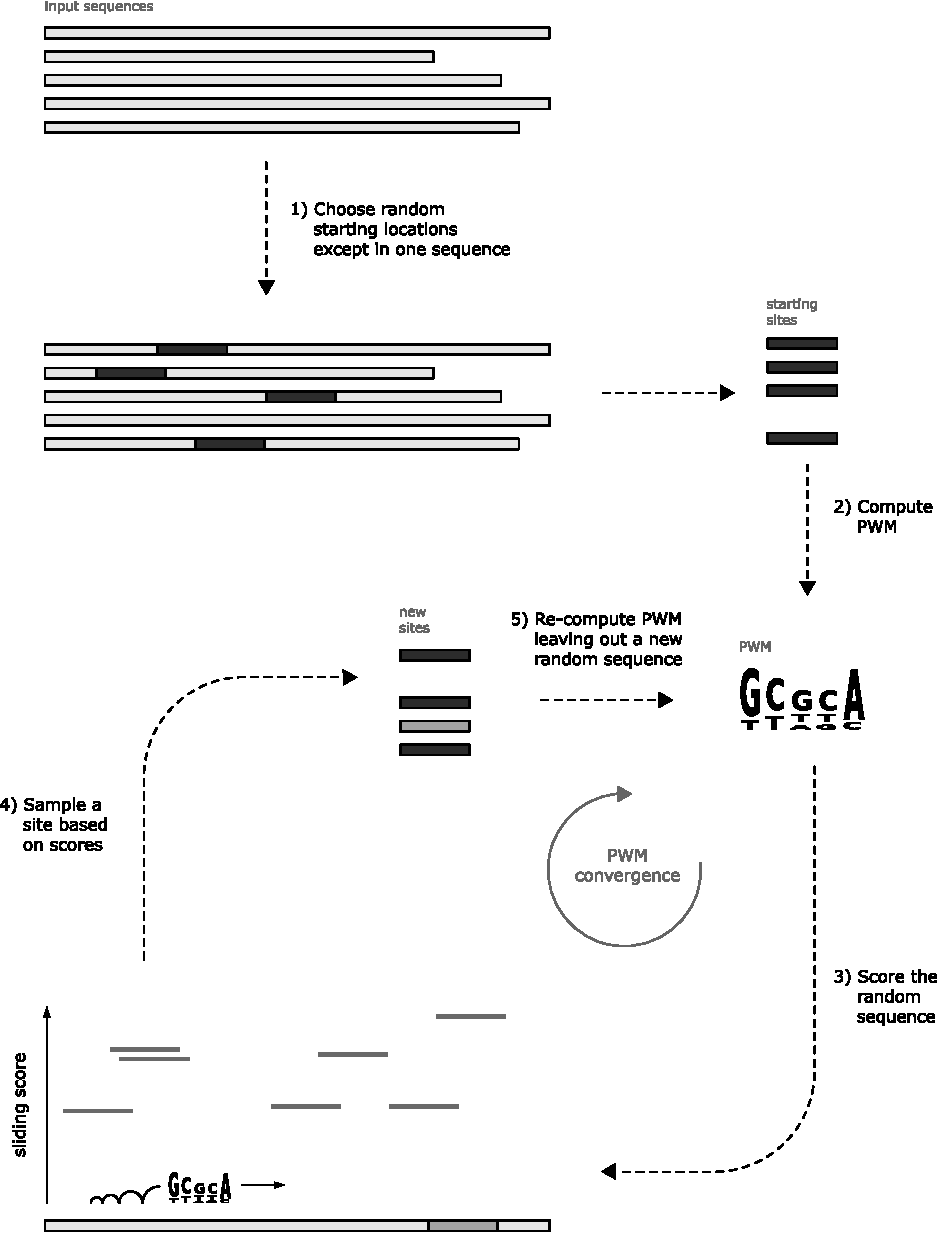
\includegraphics[height=0.80\textheight]{Body/Images-chap1/gibbs.pdf}
\caption[Schematic of the Gibbs sampling algorithm]{Schematic of the
Gibbs sampling algorithm.  As the figure shows, the Gibbs sampling
method is an iterative algorithm that progressively refines a
position weight matrix starting from a random PWM\@.  If the input
sequences contain a very strong motif, Gibbs sampling tends to
converge very quickly upon it.  However, in its original
manifestation~\cite{lawrence1993detecting}, the method was not able
to find motifs that either occurred multiple times in a single
sequence, or were found in some sequences but not others.  In
general, most motif discovery tools using PWMs bear a great deal of
similarity to the original Gibbs sampling method.
 } \label{fig:gibbs}
\end{figure}

Most of the other PWM--based motif discovery tools listed in
Table~\ref{table:pwmMD} use an approach that is similar to the Gibbs
sampler.  In general, these tools excel at finding motifs in DNA
sequences such as cis--regulatory binding sites.
(See~\citet{tompa2005assessing} for an excellent review of this
problem and a demonstration of the power of PWM--based tools.) Other
motif discovery tools use different optimization procedures than the
Gibbs sampler, which are slight variations on the MCMC method, such
as simulated annealing~\cite{kirkpatrick1983optimization} or
expectation maximization. Most of these refinement procedures
guarantee that the algorithm will converge to a
maximum~\cite{gelman1992inference}; however, it is not guaranteed
that a maximum is globally optimal. The optimization can become
trapped in a local optimum, which is called ``slow--mixing'' of the
Markov chain.  New procedures that avoid this are an active area of
study~\cite{liu2001monte}.


\begin{comment}
    Recent years have witnessed an explosive growth in the development of novel high--throughput technologies
    for probing cellular function.  These technologies have produced a flood of data, most notably from DNA and
    protein sequencing efforts, but also from metabolic phenotyping, gene expression, proteomics, and physiological
    experiments (cf.\ Figure~\vref{fig:probingCellularFunction}).  The volume of these data is so staggering as to
    defy traditional publication, leading instead to direct submission into various, increasingly bloated,
    databases such as \genbank~(cf.\ Figure~\vref{fig:genbankGrowth}).  These databases are extremely diverse and numerous, ranging from species--specific gene expression databases to databases
    for gene sequences and protein structures.

    This diversity presents a pressing question, which is central to the
    field of systems biology: How do we integrate and analyze
    these databases in a holistic and biologically meaningful manner?  Unfortunately, efforts
    to date have produced a fragmented and confusing landscape of largely database--specific analysis tools.  These overly
    specific tools are ill suited to our needs as we begin
    to pose more probing questions of biology, particularly with regard to the systemic interdependence of cells.  Instead,
    we require \emph{generic} techniques, applicable to a diverse array of data types, for elucidating biological \emph{associations}.
    In this context, ``associations'' are essentially very rudimentary statements like ``gene A is related to gene B'' or
    ``motif C is involved in apoptosis''.  Such simple statements reflect the naivety of our current understanding of
    complex biological systems; however, they can be very powerful as indicators of topics worthy of further, more specific,
    study.

    In this proposal, I will focus on \emph{syntactic pattern discovery} as a generic tool for revealing such associations
    in diverse data sets.  Broadly speaking, syntactic pattern discovery techniques are used for finding patterns in
    data that can be projected into streams of primitives.  This problem is roughly analogous to finding the syntax
    rules in a book of an unknown language.  In the context of DNA microarray data, this book may consist of expression
    levels of thousands of genes.  Or, in clinical data, this book may contain answers to lifestyle questions asked
    of cancer patients.  In the latter case, we would be looking for associations like ``people
    who \emph{smoke} and are \emph{over 50} are likely to have \emph{prostate} cancer''.  This pattern is conceptually no different
    than a functional motif in the context of protein sequences.  For example, we can use syntactic pattern discovery to find
    associations such as ``the motif `\texttt{KT..GA..R}' is associated with dehydrogenase enzymes.''

    Techniques for finding associations in data, such as syntactic pattern discovery, are extremely useful for pinpointing interesting phenomena,
    but do not seek to explain them.  As such, these techniques are sufficiently generic to find wide applicability in the diverse and copious
    databases that have become available.  The continued growth of these databases will ensure
    that techniques like syntactic pattern discovery will play a pivotal role in directing the course of biological research in the coming years.



        \begin{figure}[tbph!]
        \centering
            %\include{Body/Images-chap1/fig_cell}
        \caption[Probing Cellular Function]{Probing Cellular Function.  This figure shows just of a few of the diverse set of
        techniques available to researchers for probing the function of cells.  Due to the high--throughput nature of
        these techniques, data bases are rapidly becoming prohibitively volumous.}
        \label{fig:probingCellularFunction}
        \end{figure}

        \begin{figure}[ptbh]
        \centering
            %\include{Body/Images-chap1/fig_genbank}
        \caption[Exponential growth of \genbank ]{Exponential growth of \genbank .  \genbank~has increased by
                and order of magnitude nearly every three years and has grown to include approximately $10^{10}$ DNA base--pairs
                and $10^7$ sequences from over 55,000 different species~\cite{benson2000genbank}.}
        \label{fig:genbankGrowth}
        \end{figure}

\section{General Objectives and Specific Aims}

    \subsection{General Objectives}
        The central theme of the work proposed here is the use of
        syntactic pattern discovery techniques to find novel associations
        in biological systems.  In particular, we will focus on protein
        sequence, DNA sequence, gene expression, and physiological data
        being generated by both our own laboratory and by collaborators.
        We will use these data to solve a number of problems of both
        practical and scientific interest to the life sciences community,
        which are described in Section~\vref{subsection:specificAims}.

        The manner in which we will approach these problems, and the
        types of methods that we will employ are probably best explained
        through a few short examples.  Below, I will describe two very
        simple problems in which syntactic pattern discovery proves to be
        a powerful tool for elucidating interesting biological phenomena.
        It is important to note that, despite the qualitative difference
        between these two problems, they can be analyzed using the same
        generic framework.

        \subsubsection{A Few Simple Examples}
            \begin{description}
            \item[Breast Cancer Association Discovery:]
                Table~\vref{table:breastCancerData} shows
                a representative sampling of a larger data set containing tumor statistics from breast cancer patients.  Given data
                such as these, we are interested in finding associations between the different columns which may have some biological meaning.
                For example, in this data set, we find that patients who have rough and low--density tumors are more likely to develop recurrent
                cancers.  However, these data do not indicate that merely having a rough \emph{or} a low--density tumor is enough to predispose
                a patient to recurrence.  This suggests that there is some association between the two factors that may have
                a biological underpinning, for example a mechanism of malignant cell growth.  Such associations can be strong indicators
                of areas worthy of further study.

                \begin{table}[!hbtp]
                \centering
                \caption[Association discovery in cancer patient data]{Association discovery in cancer patient data.  These data are just a
                small fraction a complete clinical study of breast cancer patients by Mangasarian \etal~\cite{mangasarian1995breast} available in
                the University of California Irvine Machine Learning Repository~\cite{uci1998ucirepository}.  The first column indicates whether
                or not the patient's cancer returned.  All other columns contain an integer, 1--10, indicating the percentile in which the
                patient lies for a specific metric.  For instance, the first patient had a tumor that was in the $20^{\textrm{th}}$ percentile
                in area.  Using syntactic pattern discovery, we can find a number of associations in the full data set.  For example, patients
                who have very rough and low--density tumors ($10^{\textrm{th}}$ percentiles in both cases) are likely to have recurrent cancers.  However,
                these factors are not necessarily important individually; there is an association between the two.}\label{table:breastCancerData}
                    \vspace{0.2cm}
\begin{tabular}{ccccccccccc}\rule{0pt}{15mm}% vertical placement p 324 latex companion}
\begin{rotate}{45}recurrent?\end{rotate} & \begin{rotate}{45}radius\end{rotate} & \begin{rotate}{45}texture\end{rotate} &
\begin{rotate}{45}perimeter\end{rotate} & \begin{rotate}{45}area\end{rotate} & \begin{rotate}{45}smoothness\end{rotate} & \begin{rotate}{45}compactness\end{rotate} &
 \begin{rotate}{45}concavity\end{rotate} & \begin{rotate}{45}concave points\end{rotate} & \begin{rotate}{45}symmetry\end{rotate} &
  \begin{rotate}{45}fractal dimension\end{rotate}\\\hline\hline
no &  3 & 2 & 2 & 2 & 0 & 1 & 6 & 2 & 3 & 4 \\
no &  3 & 6 & 6 & 6 & 3 & 4 & 0 & 5 & 9 & 2 \\
no &  5 & 2 & 2 & 2 & 2 & 4 & 1 & 2 & 6 & 2 \\
no &  0 & 5 & 10 & 1 & 5 & 9 & 2 & 9 & 8 & 1 \\
yes &  4 & 4 & 1 & 3 & 1 & 1 & 0 & 3 & 5 & 3 \\
yes &  0 & 3 & 4 & 1 & 1 & 1 & 1 & 6 & 5 & 2 \\
no &  3 & 2 & 1 & 2 & 1 & 1 & 2 & 2 & 6 & 1 \\
yes &  1 & 1 & 5 & 2 & 1 & 1 & 3 & 5 & 4 & 3 \\
no &  0 & 4 & 5 & 1 & 2 & 2 & 4 & 6 & 6 & 1 \\
no &  0 & 5 & 6 & 0 & 5 & 1 & 7 & 7 & 7 & 5 \\
no &  2 & 0 & 1 & 1 & 0 & 1 & 5 & 2 & 2 & 1 \\\hline\hline
\end{tabular}

                \end{table}

            \item[Gene Local Homology Discovery:]Table~\vref{table:arabGenes} shows a few genes from the Arabodopsis genome.  Given sequence data, we are typically
                interested in identifying areas of similarity between two sequences or finding functional motifs.  A rigorous example
                of either of these problems requires more development.  But, in
                this very simple case, we may be interested in finding long subsequences of these gene which are present in all three.  Other
                than the poly--A tails, there are only a few such subsequences, for example \texttt{CCACGCGTCCGAAAA}.  In some problems, we
                may use such conserved regions to deduce an evolutionary history of these genes or try to correlate these regions with a
                certain function. 

                \begin{table}[!hbtp]
                \centering
                \caption[Gene sequences from Arabodopsis]{Genes sequences from Arabodopsis.  These very small genes are only a
                few hundred bases long, whereas a typical gene can be many kilo--bases in length.  At first glance, only the poly--A tails
                stand out as areas of local homology; however other long strings, such as \texttt{CCACGCGTCCGAAAA} appear in all three sequences.
                In databases that contain literally billions of these sequences, we would use syntactic pattern discovery to find these
                kinds of patterns.}\label{table:arabGenes}
                    \begin{tabular}{l}\hline\hline
$>$gi$\|$8571926 Arabidopsis thaliana lipid transfer protein \\
\ttfamily \footnotesize CCACGCGTCCGAAAAAAAAAACAGAAAGTAACATGAGATCTCTCTTATTAGCCGTGTGCCTGGTTCTTGC \\
\ttfamily \footnotesize TTTACACTGCGGTGAAGCAGCCGTGTCTTGCAACACGGTGATTGCGGATCTTTACCCTTGCTTATCCTAC \\
\ttfamily \footnotesize GTGACTCAGGGCGGACCGGTCCCAACCCTCTGCTGCAACGGTCTCACAACACTCAAGAGTCAGGCTCAAA \\
\ttfamily \footnotesize CTTCTGTGGACCGTCAGGGGGTCTGTCGTTGCATCAAATCTGCTATTGGAGGACTCACTCTCTCTCCTAG \\
\ttfamily \footnotesize AACCATCCAAAATGCTTTGGAATTGCCTTCTAAATGTGGTGTCGATCTCCCTTACAAGTTCAGCCCTTCC \\
\ttfamily \footnotesize ACTGACTGCGACAGTATCCAGTGAGACAAGCAGAAAATCTTAAAGGAAGCTACTACAAGAACTATAATAA \\
\ttfamily \footnotesize CCTAATAATTAATAAATGAGGGCATTGGTTTGCTAGTTGCTAATTGATCAGTGATGTATTGTCATTTTGA \\
\ttfamily \footnotesize ATGTTCTAATATCAGCAGGCACTTATCTCTGAAAAAAAAAAAAAAAA \\ \\
$>$gi$\|$8571922 Arabidopsis thaliana lipid transfer protein \\
\ttfamily \footnotesize CCACGCGTCCGAAAACACAAGCGTAGAAAACAAAACTCAACTAATTGTGTTATCACCCAAAAGAGAAGAG \\
\ttfamily \footnotesize CAAACACAATGGCTTTCGCTTTGAGGTTCTTCACATGCTTTGTTTTGACAGTGTTCATCGTTGCATCAGT \\
\ttfamily \footnotesize GGATGCAGCAATAACATGTGGCACAGTGGCAAGTAGCTTGAGTCCATGTCTAGGCTACCTATCGAAGGGT \\
\ttfamily \footnotesize GGGGTGGTGCCACCTCCGTGCTGTGCAGGAGTCAAAAAGTTGAACGGTATGGCTCAAACCACACCCGACC \\
\ttfamily \footnotesize GCCAACAAGCATGCAGATGCTTACAGTCCGCTGCAAAAGGGGTTAATCCAAGTCTAGCCTCTGGCCTTCC \\
\ttfamily \footnotesize TGGAAAGTGCGGTGTTAGCATCCCCTATCCCATCTCCACGAGCACCAACTGCGCCACCATCAAGTGAAGT \\
\ttfamily \footnotesize GGGGAATAACGACATCATTTGCCTGAAGAGTATGGTTTCGTATACGTAAAATAAGACGGCTATCTAAGCT \\
\ttfamily \footnotesize GATATTTACCTTGTCTTTGTTTGTCTTGATGGCTTTGTAATCTTTTGCTTTGTTATGTTGTATACTTGTG \\
\ttfamily \footnotesize TCTTAACATGTTTAAGATATGATAATATATAGTATCGGTACCTTATTAAAAAAAAAAAAAAA \\ \\
$>$gi$\|$8571922 Arabidopsis thaliana lipid transfer protein \\
\ttfamily \footnotesize CCACGCGTCCGAAAACACAAGCGTAGAAAACAAAACTCAACTAATTGTGTTATCACCCAAAAGAGAAGAG \\
\ttfamily \footnotesize CAAACACAATGGCTTTCGCTTTGAGGTTCTTCACATGCTTTGTTTTGACAGTGTTCATCGTTGCATCAGT \\
\ttfamily \footnotesize GGATGCAGCAATAACATGTGGCACAGTGGCAAGTAGCTTGAGTCCATGTCTAGGCTACCTATCGAAGGGT \\
\ttfamily \footnotesize GGGGTGGTGCCACCTCCGTGCTGTGCAGGAGTCAAAAAGTTGAACGGTATGGCTCAAACCACACCCGACC \\
\ttfamily \footnotesize GCCAACAAGCATGCAGATGCTTACAGTCCGCTGCAAAAGGGGTTAATCCAAGTCTAGCCTCTGGCCTTCC \\
\ttfamily \footnotesize TGGAAAGTGCGGTGTTAGCATCCCCTATCCCATCTCCACGAGCACCAACTGCGCCACCATCAAGTGAAGT \\
\ttfamily \footnotesize GGGGAATAACGACATCATTTGCCTGAAGAGTATGGTTTCGTATACGTAAAATAAGACGGCTATCTAAGCT \\
\ttfamily \footnotesize GATATTTACCTTGTCTTTGTTTGTCTTGATGGCTTTGTAATCTTTTGCTTTGTTATGTTGTATACTTGTG \\
\ttfamily \footnotesize TCTTAACATGTTTAAGATATGATAATATATAGTATCGGTACCTTATTAAAAAAAAAAAAAAA \\\hline\hline
\end{tabular}

                \end{table}
                \end{description}

    \subsection{Specific Aims}\label{subsection:specificAims}
        The work proposed here has two specific goals:
        \begin{enumerate}
            \item   To use syntactic pattern discovery in the space of protein and DNA sequences.  Specifically, we will
                    develop a model of protein molecular evolution based on large--scale syntactic pattern discovery in
                    the set of natural proteins.  Also, we will develop a method for predicting cDNA oligonucleotide
                    hybridization kinetics and selecting optimal probes for DNA microarrays using syntactic pattern
                    discovery.
            \item   To elucidate novel biological associations in expression and physiological data.  Using data that
                    is being generated in our own laboratory and by collaborators, we will apply syntactic pattern discovery
                    to create leads for further, in--depth, research.  We will pay particular attention to a few model systems
                    including diabetes and various cancers.
        \end{enumerate}




\section{Tools for Pattern Discovery}
    \subsection{Introduction}\label{pdIntro}
        The general pattern discovery problem is as follows: given a data
        set, find the underlying patterns in the data.  Depending on what
        we mean by a ``pattern'' and what kinds of data we are given,
        this problem can take on many forms.  Figure~\vref{fig:gaussian}
	shows a very simple pattern discovery problem
        in which we use a clustering technique to find patterns.

        It is important to distinguish between pattern \emph{discovery} and pattern \emph{recognition}.  In pattern
        recognition we are given patterns and we search for occurrences of these patterns in a data set.  This, relatively
        simple, task is closely associated with the concept of classification in which we partition the data set into groups
        depending on which patterns the data match.  Pattern discovery is essentially the inverse of pattern
        recognition and is a much more difficult task: given the data, find the groups.



        From Figure~\vref{fig:gaussian}, it is obvious that there are many different ways to answer the
        pattern discovery problem depending on our predefined notion of what a pattern should look like.  For example,
        we may say that a pattern is a collection of dots that lie within a circle of a certain radius.  Or, we could
        say that a pattern is a set dots in which each dot is no more than a certain distance away from every other dot.
        Essentially, we need to define the
        pattern \emph{class} for which we will look.  This is an fundamental tenet of the general pattern discovery problem.

        In this work, we will deal exclusively with data that consists of sequences of characters; however, the underlying
        principles of pattern discovery remain unchanged.  For example, given two character strings, ``\texttt{thesiscommittee}''
        and ``\texttt{iscommitted}''\footnote{As in, the ``\texttt{thesiscommittee}'' ``\texttt{iscommitted}'' to getting me out in a minimal amount of time.}, what are the patterns is these strings?  One answer is that they both contain letters from the
        set \{\texttt{t,h,e,s,c,o,m,i,t}\}.  Another answer is that they both contain the substring ``\texttt{iscommitte}'', and yet
        another answer is that they both contain the substring ``\texttt{commit}''.  Depending on how exactly we choose the
        pattern class in which we are interested, all of these answers are correct.  This concept will be discussed further in
        Section~\vref{pdIntro}.

        In what follows, I will briefly highlight a number of pattern discovery tools, distinguishing between two types: decision--theoretic
        pattern discovery tools and tools for syntactic pattern discovery.  Then, I will give a review of the \teiresias~algorithm,
        which will be the pattern discovery tool of choice for the work proposed herein.

    \subsection{Decision--Theoretic Pattern Discovery }
        Decision--theoretic pattern discovery refers to a wide variety of techniques that operate, in general, on data
        which is in vector form.  These techniques can be divided into three main areas depending on how pattern classes
        are determined: decision functions, distance functions, and likelihood functions~\cite{tou1974pattern}~\cite{duda1973pattern}.  The reader is probably most
        familiar with decision--theoretic pattern discovery techniques such linear discriminant analysis, K--means clustering,
        and hierarchical clustering.  Each of these are appropriate for elucidating different pattern classes and typically
        find most use on different forms of data.

        The most important, distinguishing, characteristic of decision--theoretic pattern discovery algorithms is that
        they are used for finding patterns in vector data.  Thus, many of these techniques are widely applicable and
        have been thoroughly exploited in the biology literature.  For example, various clustering techniques have been
        very useful for analyzing gene expression experiments.  However, these same techniques find very little use
        in sequence analysis.


    \subsection{Syntactic Pattern Discovery }
        \subsubsection{Introduction}
            Syntactic pattern discovery is the task of finding patterns in streams of primitives.  Usually, these streams
            are strings of characters, for example amino acids in a protein sequence.  However, any data set that can be
            written in terms of primitives is well--suited for syntactic pattern discovery.  For example, given the expression
            level of a gene, we may call it ``up--regulated'', ``down--regulated'', or ``no change''.  So, a sequence of
            gene expression data may be written as ``\texttt{U D N U U U D}'', where ``\texttt{U}'', ``\texttt{D}'',
            and ``\texttt{N}'' are the primitives that make up our data stream.  Given a few such streams like
            ``\texttt{U D N U U U D}'', ``\texttt{D D N U D U U}'', and ``\texttt{D D U U N U N}'',
            we would use syntactic pattern to discovery that genes 2, 4, and 6 are always expressed as ``\texttt{D}'', ``\texttt{U}'',
            and ``\texttt{U}'' together, respectively --- they are co--regulated.

            The underlying framework of syntactic pattern discovery can be traced back to Chomsky's work on syntax theory~\cite{chomsky1957syntactic,chomsky1965aspects,chomsky1956three}.
            Chomsky's work is the basis for much of formal language theory and computational linguistics.  However, in general,
            most work in these areas has been syntactic pattern \emph{recognition}, and has focused on machine learning techniques
            for computer understanding of natural languages.  Only recently have these pattern recognition techniques been applied to problems of
            interest to biologists~\cite{searls1997linguistic,searls2001reading,searls1992thecomputational}, such as gene finding.

            Though descended from formal language theory, syntactic pattern discovery has evolved independently
            in the field of computational biology through efforts in the area of sequence analysis.  In general, the
            goal of syntactic pattern discovery in biological sequence data is to find patterns or motifs that may
            have biological significance.  For example, using the \teiresias~\cite{rigoutsos1998combinatorial} syntactic pattern
            discovery algorithm, Rigoutsos \etal~\cite{rigoutsos1999dictionary} searched the SWISS--PROT/TrEMBL~\cite{bairoch2000swiss-prot} protein sequence database
            for important patterns and found many motifs such as ``\texttt{G..G.GK[ST]TL}'' (see Section~\ref{pdIntro} for
            an description of this notation), which is the well--known ATP/GTP binding P--loop.

            In what follows, I will briefly introduce some common nomenclature and notation used in the syntactic pattern
            discovery literature.  Then, I will describe the different types of syntactic pattern discovery algorithms
            that have been developed, focusing in particular on the \teiresias~algorithm.


        \subsubsection{Definitions}\label{synPdIntro}

            We define an alphabet of all characters to be $\Sigma$, where $\Sigma$ is usually either the alphabet of all possible
            amino acids or the alphabet of nucleotides.  Then a sequence $s_i$ is a string consisting of zero or more of the
            letters from $\Sigma$.  We denote this by $s_i\in\Sigma^{\ast}$, which means ``string $s_i$ is an element of the
            set of strings consisting of zero or more letters'', where the ``$\ast$'' denotes ``zero or more''.

            The generic problem of pattern discovery is, given a set
            of sequences $S = \{ s_1,s_2,\ldots,s_n\}$, and an integer
            $K$, find all patterns which occur at least $K$ times
            in $S$.  We call this set of patterns $\mathcal{C}$, where
            $\mathcal{C}=\{ p_1,p_2,\ldots,p_m\}$ and $p_i$ is a pattern
            in $\mathcal{C}$.  Each pattern $p_i$ defines a language
            $\mathcal{L}\paren{p_i}$ which is the set of all strings that
            can be derived from $p_i$.  A sequence ``matches'' $p_i$ if it
            contains a substring that belongs to $\mathcal{L}\paren{p_i}$.
            For example, if $p_i=$``\texttt{KYLE}'', then the sequences
            ``\texttt{GOTOBEDKYLE}'', ``\texttt{WRITEYOURPROPOSALKYLE}'',
            and ``\texttt{GOODBOYKYLEWRITE}'' all match $p_i$.

            As mentioned in Section~\vref{subsection introduction tools
            for pat disc}, to completely determine the pattern discovery
            problem, we have to specify the pattern class in which we are
            interested.  This pattern class determines the form of each
            $p_i$ that we find.  Below, a few pattern classes, commonly
            used in biological sequence analysis,  are enumerated in
            order of increasing complexity~\cite{floratos1999pattern}:

            \begin{itemize}
                \item   $p_i\in\Sigma^{\ast}$:  This is the class
                        of all ``solid'' patterns, for example
                        ``\texttt{KAGTPT}'' and ``\texttt{TAGCGGGAT}''.

                \item   $p_i\in(\Sigma\cup\{.\})^{\ast}$:  This is the
                        class of all patterns that can have ``wildcard''
                        positions, which are denoted by ``.'', for example
                        ``\texttt{K.G.PT}'' and ``\texttt{TA...GGAT}''.
                        The wildcard means that any character from the
                        alphabet will suffice in that position.

                \item   $p_i\in(\Sigma\cup R)^{\ast}$: This
                        is the class of all patterns that can
                        have ``bracketed'' expressions, for
                        example ``\texttt{K[ADG]G[KQ]PT}'' and
                        ``\texttt{TA[GA][TC]GGAT}''.  The bracketed
                        expression ``[\texttt{TC}]'' means that either
                        ``\texttt{T}'' or ``\texttt{C}'' will suffice in
                        that position.  In this notation, $R$ represents
                        the set of characters in the brackets, for example
                        $R=\{\texttt{TC}\}$ or $R=\{\texttt{GA}\}$.

                \item   $p_i\in(\Sigma\cup X)^{\ast}$:  This is the
                        class of ``flexible'' patterns.  For example
                        ``\texttt{Kx(1,3)Gx(2,5)PT}'', where ``x(2,5)''
                        means that anywhere between two and five wildcards
                        can exist at that position, that is x(2,5)
                        can be any one of $\{..,...,....,......\}$.

            \end{itemize}
            In general, the more complex these patterns are, the more expressive the languages will be that we find.  However,
            with increasing complexity, the computational difficulty of the pattern discovery problem increases
            drastically~\cite{maier1978complexity,garey1979computers}.

            There are three characteristics that distinguish between various syntactic pattern discovery algorithms, which are as
            follows:
            \begin{enumerate}
                \item   The pattern class complexity.
                \item   The completeness of the returned pattern set.  That is, does the algorithm return \emph{all}
                        patterns present in the input sequences?
                \item   The pattern \emph{maximality}.  For instance, in the two strings ``\texttt{KYLEJ}'' and ``\texttt{KYLEL}'',
                        the pattern ``\texttt{KYLE}'' is maximal, whereas ``\texttt{KYL}'' is not, because we could
                        add an ``\texttt{E}'' without decreasing the number of times it occurs.
            \end{enumerate}

        \subsubsection{Syntactic Pattern Discovery Algorithms}\label{subsubsection: syntax pattern disc algos}

            There are two principal classes of algorithms used for syntactic pattern discovery in biological sequences:
            sequence driven and pattern driven algorithms~\cite{brazma1998pattern}.  Sequence driven algorithms align a set of strings,
            which are presumed to be similar, producing a ``consensus sequence''~\cite{gusfield1997algorithms}.   This consensus sequence is, in essence,
            an average of the input sequences and is used to capture patterns in the input sequences (cf.\ Figure~\vref{fig:consensusSequence})\cite{neville1997enumerating}.  The most well--known sequence driven syntactic
            pattern discovery algorithm is BLOCKS~\cite{henikoff1991automated}, others include EMOTIF~\cite{neville1997enumerating} and
            algorithms by Martinez~\cite{martinez1988flexible}, Smith \etal~\cite{smith1990automatic}, Vingron \etal~\cite{vingron1991motif},
            Shinohara~\cite{shinohara1982poly}, Nix~\cite{nix1984editing}, Roytberg~\cite{roytberg1992search}, Schuler~\cite{schuler1991workbench},
            Brodsky~\cite{brodsky1992mathematical}, and Clift~\cite{clift1986sequence}.

            Sequence driven syntactic pattern discovery algorithms, because they allow for insertions and deletions, are capable of finding
            relatively complex flexible patterns~\cite{floratos1999pattern}.  Also, by using common sequence alignment tools, which use heuristical short--cuts, they typically
            have low run--time costs.  However, because a number of input sequences are required to produce a single consensus sequence, these pattern discovery
            algorithms typically are not guaranteed to find \emph{all} the patterns.  Additionally, sequence driven algorithms are not
            guaranteed to be maximal.  As such, these algorithms are best--suited to situations in which the input sequences are known to be
            globally similar and finding all of the patterns is not important.

            \begin{figure}[tbph!]
            \centering
                %\include{fig/fig_consensus}
            \caption[Alignment with a consensus sequence]{Alignment with a consensus sequence.  Alignment--based syntactic pattern
            discovery algorithms use the consensus sequence to extract patterns from the input sequences.  In this figure, characters
            that are conserved in all sequences are capitalized.  Note that the consensus
            sequence ``{\ttfamily abd\textbf{F}l\textbf{R}-\textbf{P}abd\textbf{F}l\textbf{T}-\textbf{Q}}'' shows the pattern
            ``{\ttfamily ...F.R.P...F.T.Q}''.}
            \label{fig:consensusSequence}
            \end{figure}

            Pattern driven syntactic pattern discovery algorithms work by first enumerating possible patterns and then checking
            for the patterns in the sequence set~\cite{brazma1998pattern}.  In contrast to sequence driven algorithms, it is possible in this case to
            guarantee the completeness of the set of returned patterns.  However, this guarantee comes at the price of increased
            time and space complexity.  That is, the set of all possible patterns is very large and can take a large space
            to enumerate and a long time to search through\footnote{In fact, for arbitrarily complex patterns, this problem is
            NP--hard~\cite{garey1979computers,maier1978complexity}}.  As such, most pattern driven pattern discovery algorithms use
            heuristics to limit the space of patterns that are searched.  Common pattern driven algorithms include those by
            Queen \etal~\cite{queen1982improvements}, Waterman \etal~\cite{waterman1984pattern}, Staden~\cite{staden1989methods},
            Wolferstetter \etal~\cite{wolferstetter1996identification}, Smith \etal~\cite{smith1990finding}, Sagot \etal~\cite{sagot1997multiple},
            Suyama \etal~\cite{suyama1995searching}, Neuwald \etal~\cite{neuwald1994detecting}, Jonassen \etal~\cite{jonassen1995finding} and
            Floratos and Rigoutsos~\cite{floratos1999pattern,rigoutsos1998combinatorial}.



    \section{Papers to consider}
	\citet{yaffe2001motif}\\
	\citet{scott2004predicting}\\
	\citet{buck2005networks}\\
	\citet{robinson2004simple}\\
	\citet{yang2004predicting}\\
	\citet{pearson1990rapid}\\
	\citet{pearson1991searching}\\
	\citet{maier1978complexity}\\
	\citet{salgado2004regulondb}\\
	\citet{prakash2005statistics}\\
	\citet{tompa2005assessing}\\
	\citet{venter2001sequence}\\
	\citet{lander2001initial}\\
	\citet{browning2004regulation}\\
	\citet{zhang2000greedy}\\
	\citet{wheeler2005database}\\
	\citet{styczynski2004extension}\\
	\citet{eddy1998profile}\\
	\citet{garey1979computers}\\
	\citet{stormo1982use}\\
	\citet{stormo1982use}\\
	\citet{staden1984computer}\\
	\citet{duda2000pattern}\\
	\citet{heger2003sensitive}\\
	\citet{tomita1989optimal}\\
	\citet{zaki2000scalable}\\
	\citet{murthy2003rnabase}\\
	\citet{eskin2002finding}\\
	\citet{keich2002finding}\\
	\citet{keich2002subtle}\\
	\citet{price2003finding}\\
	\citet{thompson1994clustal}\\
	\citet{kabsch1983dictionary}\\
	\citet{williams2003multiple}\\
	\citet{bajic2004promoter}\\
	\citet{eddy2004how}\\
	\citet{bateman2004pfam}\\
	\citet{bairoch2000enzyme}\\
	\citet{marchler2003cdd}\\
	\citet{kel2004recognition}\\
	\citet{sinha2003discriminative}\\
	\citet{sinha2003ymf}\\
	\citet{lee2003generating}\\
	\citet{haverty2004cisml}\\
	\citet{fu2004motifviz}\\
	\citet{frith2004detection}\\
	\citet{poluliakh2003melina}\\
	\citet{frith2004finding}\\
	\citet{jonassen2002structure}\\
	\citet{stormo2000dna}\\
	\citet{lepre2004genes}\\
	\citet{mancheron2003pattern}\\
	\citet{hofacker2004alignment}\\
	\citet{wingender2000transfac}\\
	\citet{sinha2000statistical}\\
	\citet{sinha2003performance}\\
	\citet{pevzner2000combinatorial}\\
	\citet{duda1973pattern}\\
	\citet{tou1974pattern}\\
	\citet{hertz1999identifying}\\
	\citet{henikoff1995automated}\\
	\citet{lawrence1993detecting}\\
	\citet{bailey1994fitting}\\
	\citet{jonassen1995finding}\\
	\citet{agrawal1995mining}\\
	\citet{altschul1990basic}\\
	\citet{altschul1991amino}\\
	\citet{altschul1996local}\\
	\citet{altschul1997gapped}\\
	\citet{bradley2002trilogy}\\
	\citet{brazma1997approaches}\\
	\citet{brazma1998predicting}\\
	\citet{buhler2001finding}\\
	\citet{burge2000prediction}\\
	\citet{chomsky1956three}\\
	\citet{dayhoff1979amodel}\\
	\citet{dehal2002thedraft}\\
	\citet{dhaeseleer2000genetic}\\
	\citet{dsouza1997searching}\\
	\citet{floratos1999pattern}\\
	\citet{guhathakurta2002identifying}\\
	\citet{henikoff1991automated}\\
	\citet{henikoff1992aminoacid}\\
	\citet{hughes2000computational}\\
	\citet{jonassen1996methods}\\
	\citet{jurafsky2000speech}\\
	\citet{karlin1990methods}\\
	\citet{kim2003bioinformatic}\\
	\citet{levy1998xlandscape}\\
	\citet{li2001selection}\\
	\citet{lin2002finding}\\
	\citet{liu2001functional}\\
	\citet{manber1993suffix}\\
	\citet{parida1998musca}\\
	\citet{pearson1998improved}\\
	\citet{pedersen1999thebiology}\\
	\citet{pesole2000patsearch}\\
	\citet{rigoutsos1998combinatorial}\\
	\citet{rigoutsos1999dictionary}\\
	\citet{rigoutsos2000theemergence}\\
	\citet{searls1992thecomputational}\\
	\citet{searls2002language}\\
	\citet{smith1981identification}\\
	\citet{waterman1984efficient}\\
	\citet{wootton1993statistics}\\
	\citet{yaffe2001motif}\\


\end{comment}


\chapter{Design of antimicrobial peptides}\label{chapter:amps}

\section{Introduction}
    In the previous chapter, I introduced grammars as a generalized
    method for modeling motifs in sequences of characters.  In
    addition, I presented a detailed look at the Teiresias motif
    discovery tool.  In this, the second chapter of my thesis, I
    show how Teiresias can be used to derive sets of regular
    grammars describing a particular class of protein sequences ---
    antimicrobial peptides.  In what follows, I present a general
    background on antimicrobial peptides and then provide a
    rationale for why these peptides are particularly well--suited
    for being modeled using regular grammars.  I detail the
    construction of an annotation tool for finding new antimicrobial
    peptides and validating the general hypothesis that regular
    grammars can be used as a sensitive and specific indicator of
    antimicrobial function in peptide sequences.  Next, I describe
    the preliminary design of synthetic antimicrobial peptides using
    an evolutionary approach, which, although ultimately inconclusive, provided
    motivation for a more focused design.  The final section of this
    chapter describes a more focused design approach, detailing the
    successful construction of numerous novel peptides with strong
    antimicrobial activity against a wide spectrum of bacteria.

    The research described in this chapter is drawn
    largely from a publication that is in preparation
    in collaboration with Christopher Loose, Isidore
    Rigoutsos, and Gregory Stephanopoulos.  (Some
    experimental work in Section~\vref{section:preliminary}
    was also performed by Gyoo Yeol Jung.)  Throughout this
    chapter, the use of the pronoun ``we'' refers to this
    group of authors.

\section{Motivation}
    Antimicrobial peptides are small
    proteins that attack and kill microbes.
    These peptides are effectors of the
    innate immune system: the phylogenetically
    ancient first line of defense against pathogen
    assault~\cite{rolff2003invertebrate,kimbrell2001evolution}.
    Antimicrobial peptides are ubiquitous
    amongst multicellular eukaryotes and
    found in diverse contexts including frog
    skin~\cite{simmaco1999antimicrobial}, scorpion
    venom~\cite{moerman2002antibacterial}, and human
    sweat~\cite{schittek2001dermcidin}.

    There is a growing interest in antimicrobial
    peptides, due largely to the proliferation
    of multi--drug resistant pathogen
    strains~\cite{cassell2001development}.  These
    strains are resistant to one or more common
    antibiotics such as penicillin, tetracylin,
    or vanocomycin.  In the United States alone,
    the cost of treating and preventing infections by
    these pathogens is estimated to be many billions of
    dollars annually~\cite{harrison1998antimicrobial}.
    In the arms race against microbes,
    mankind is losing --- only a single new
    class of antibiotics was developed in the
    past 30 years~\cite{normark2002evolution,
    walsh2000molecular}.  However, there is mounting
    evidence that antimicrobial peptides are less
    likely to induce bacterial resistance and will make
    a strong contribution to our therapeutic arsenal
    ~\cite{zasloff2002antimicrobial,zasloff2002antimicrobialpeptides,ge1999invitro}.

    Human antimicrobial peptides, such as
    the defensins and cathelicidins, help to
    maintain a passive defense against pathogens
    in the environment.  A malfunction of these
    peptides leads to severely immunocompromised
    phenotypes.  For example, a deficiency of the
    LL-37 cathelicidin leads to morbus Kostmann,
    a congenital neutropenia characterized
    by recurrent bacterial infection and short
    life--expectancy~\cite{putsep2002deficiency,bowman2003antibacterial}.
    In addition, the pathogenesis of cystic fibrosis
    (CF) is indirectly caused by antimicrobial peptide
    impairment~\cite{ganz2003defensins}.  CF patients
    have a defective Cl$^-$ ion channel in the
    pulmonary airway epithelia that causes unusually
    high salt concentrations.  The salt disrupts the
    function of the epithelial defensins, leading
    to chronic infections and ensuing respiratory
    failure~\cite{smith1996cystic,zasloff2002antimicrobial}.
    More severe phenotypes have been produced in
    loss--of--function animal models.  For example,
    Wilson \emph{et. al.}~\cite{wilson1999regulation}
    showed that mice with depressed defensin
    activity required a 10--fold lower dose
    of the \emph{S. typhimurium} pathogen
    to produce a fatality.  In contrast,
    gain--of--function mice expressing human
    enteric defensin HBD--5 have a markedly
    increased resistance to \emph{S. typhimurium}
    assault~\cite{salzman2003protection}.

    In addition to their more publicized
    antibiotic capabilities, antimicrobial peptides
    appear to be important in a variety of other
    diseases.  For example, the antimicrobial
    peptides of \emph{Anopheles gambiae},
    the malaria mosquito, are upregulated
    after malaria (\emph{Plasmodium berghei})
    infection~\cite{christophides2002immunity}
    and, in some cases, are capable
    of killing the ookinetes of the
    parasite~\cite{barillas2000mosquito,vizioli2001gambicin}.
    Antimicrobial peptides are also indicated in a
    resistance to the AIDS--causing virus, HIV\@.
    Long--term HIV nonprogressors display
    elevated levels of $\alpha$--defensins
    that inhibit the proliferation of the
    virus~\cite{zhang2002contribution}.
    Finally, a limited class of antimicrobial
    peptides may form the basis for novel cancer
    treatments~\cite{kim2003invitro,ellerby1999anticancer}.
    For example, the antimicrobial peptide
    tachyplesin can repress the growth of cancerous
    tumors both \emph{in vitro} and \emph{in
    vivo}~\cite{chen2001rgdtachyplesin}.

    The many disease--relevant behaviors of
    antimicrobial peptides are a result of their
    ability to broadly distinguish eukaryotic
    cells from pathogenic invaders.  There are two
    features that give the peptides this ability:
    a net positive charge and an amphipathic 3--D
    structure~\cite{giangaspero2001amphipathic,epand1999diversity}.
    These features endow the peptide with an
    affinity for negatively charged outer leaflet
    of the bacterial cytoplasmic membrane (see
    Figure~\vref{fig:peptideAction}).  This affinity
    leads to permeablization of the bacterial membrane,
    which is the basis for the bactericidal activity
    of antimicrobial peptides.  Although this mode
    of action is common to almost all antimicrobial
    peptides, there are many diverse primary sequences
    that can produce this behavior.  These sequences
    form a handful of conserved families, the most
    common of which are the $\alpha$--helical
    and $\beta$--sheet antimicrobial peptides
    ~\cite{tossi2000amphipathic}.

    \begin{figure}[phtb] \centering
    \includegraphics[width=0.70\textwidth]{Body/Images-chap2/attack2.png}
    \caption[Antimicrobial peptide action]{
        Antimicrobial peptide action.  In the
        figure above, amphipathic antimicrobial
        peptides with net positive charges are
        attracted via electrostatic forces to
        the negatively charged outer--leaflet
        of the microbial membrane (step
        1)~\cite{zasloff2002antimicrobial}.  This
        membrane is either the lipopolysaccharide
        layer or the peptidoglycan layer of
        gram--negative and gram--positive bacteria,
        respectively~\cite{epand1999diversity}.
        In addition, the $\beta$--1,3--glucan in
        fungal membranes and the phosphoglycan
        of certain parasites can give membrane
        characteristics that are exploited
        by certain classes of antimicrobial
        peptides.  The peptides cover and lyse
        the membrane via either a ``barrel
        stave'' or ``carpet'' mechanism (step
        2)~\cite{shai2002mode}.  Although some
        antimicrobial peptides are hemolytic,
        in general, they are not damaging to
        multicellular organisms because 1) the
        negatively charged phosphatydilserines
        of their outer leaflet are sequestered
        on the cytoplasmic side of the membrane,
        and 2) the membranes are stabilized by
        cholesterols~\cite{zasloff2002antimicrobial}.
    } \label{fig:peptideAction} \end{figure}


Figure~\vref{fig:aurein} shows the structure of aurein--1.2, an
archetypal alpha helical antimicrobial peptide from the Australian
Southern bell frog~\cite{wang2005correlation}.  Alpha helical AmPs
form the largest single family of AmPs.  They are particularly
common in amphibians because species such as frogs tend to inhabit
wet and warm ecological niches that are conducive to the
proliferation of bacteria.  (See Figure~\ref{fig:frogAmps} for a
phylogenetic tree of the more than 400 amphibian AmPs.)  Alpha
helical AmPs tend, in general, to have a amphipathic structure in
which positively charged residues are segregated on to a particular
side of the longitudinal axis of the helix.  Negatively charged or
neutral residues tend to be isolated on the opposite side from the
positively charged residues.  Evidence suggests that this
confirmation allows the peptide to position itself judiciously
relative to the bacterial membrane, facilitating entry of the
peptide into the membrane and, ultimately, membrane
disruption~\cite{zasloff2002antimicrobial}.

        \begin{figure}[ptb]
        A) Ball and stick
        \begin{center}
        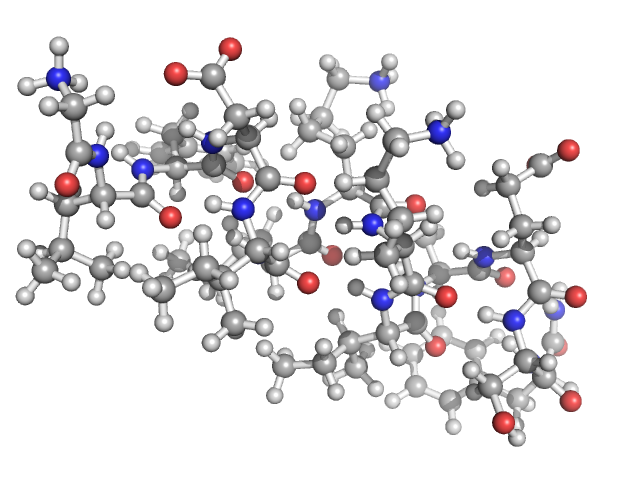
\includegraphics[width=2.0in]{Body/Images-chap2/1vm5-balls.png}
        \end{center}

        \smallskip
        B) Ribbon
        \begin{center}
        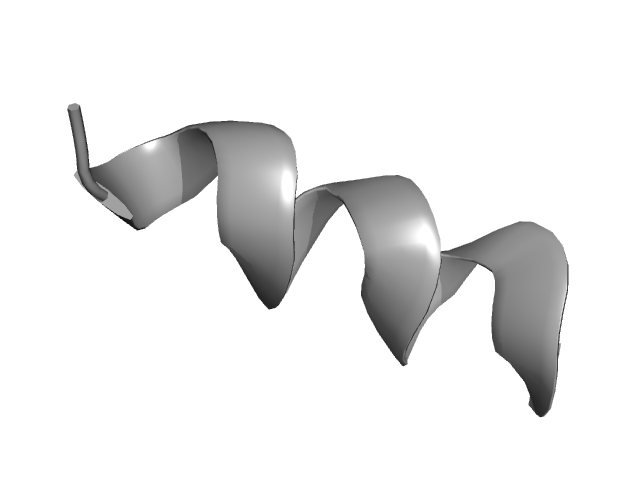
\includegraphics[width=2.0in]{Body/Images-chap2/1vm5-ribbon.png}
        \end{center}

        \smallskip
        C) Peptide wheel view
        \begin{center}
        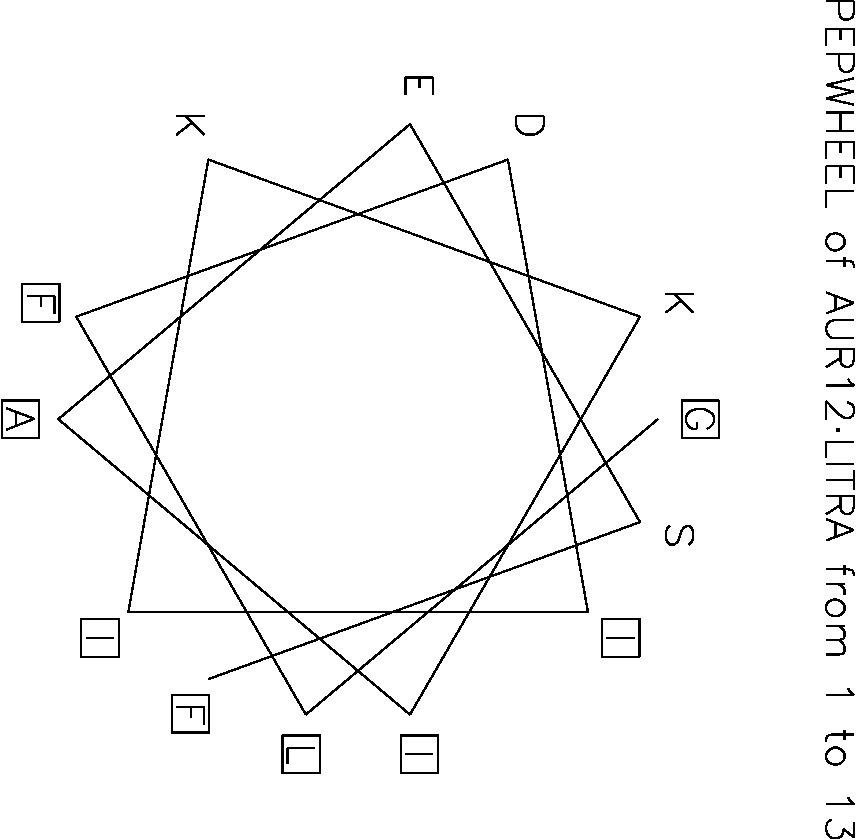
\includegraphics[angle=90,width=2.0in]{Body/Images-chap2/pepwheel.pdf}
        \end{center}
        \caption[The structure of aurein]{The structure of aurein--1.2~\cite{wang2005correlation}.
            Aureins constitute a large family of secreted proteins
            originally isolated from the skin of frogs.
            This particular structure was isolated from the
            Australian Southern bell frog.  The peptide conforms to
            the classic amphipathic alpha helical structure and has wide--spectrum antimicrobial activity.
            Part A) shows a ball--and--stick representation of the
            structure in which nitrogen atoms are colored blue and
            oxygen atoms are colored red.  Part B) shows the same
            structure using a cartoon representation that clearly
            shows the alpha helix.  Finally, part C) shows a helical
            wheel projection in which uncharged residues are boxed
            in order to highlight the segregation of charges on the
            helix.  Graphics created using PyMol (DeLano Scientific,
        San Carlos, CA, USA).
        }
        \label{fig:aurein}
        \end{figure}

        \begin{sidewaysfigure}[ptb]
        \begin{center}
        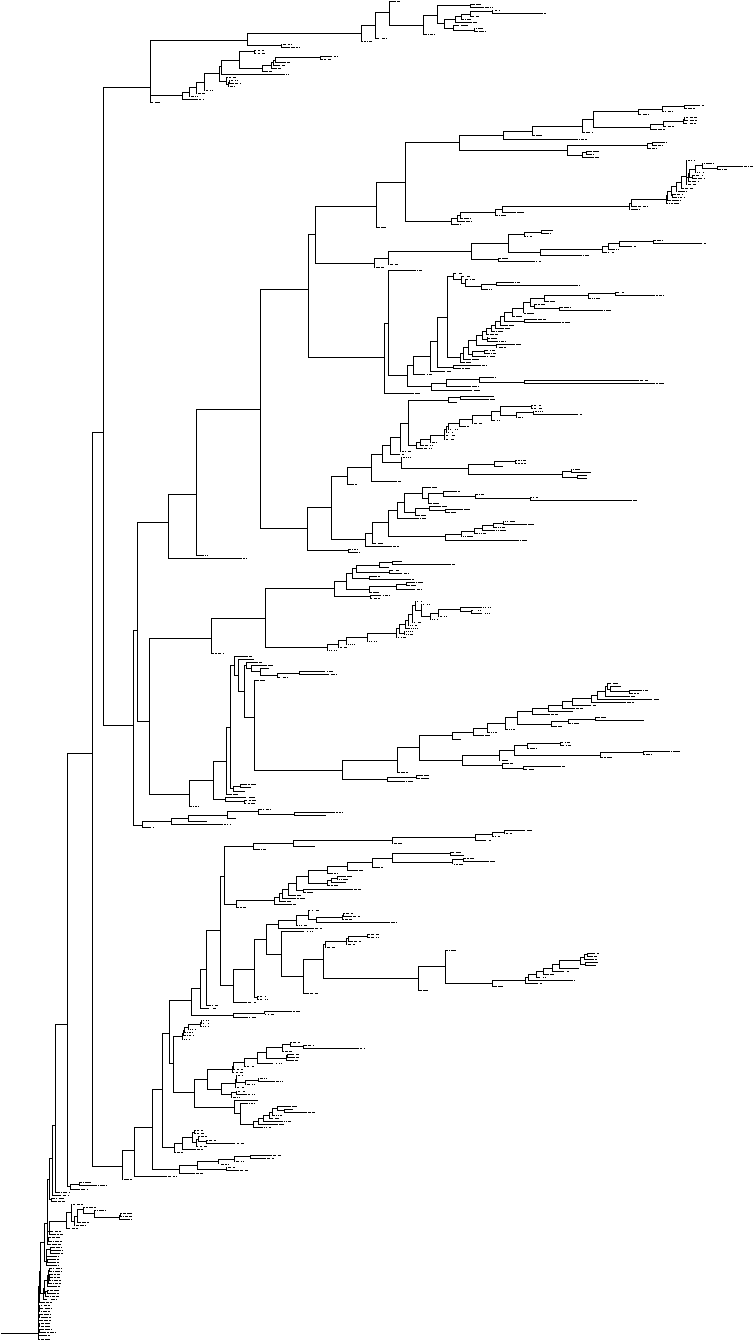
\includegraphics[angle=270,width=0.9\textwidth]{Body/Images-chap2/frog-amps.pdf}
        \end{center}
        \caption[A phylogenetic tree of amphibian antimicrobial peptides]{
            A phylogenetic tree of amphibian AmPs.  Because they
            tend to inhabit environments that are conducive to the
            growth of bacteria, amphibians are under evolutionary
            pressure to develop numerous and varied AmPs.  This tree
            shows the degree of sequence similarity for over 400
            AmPs isolated from amphibian sources.  As the figure
            shows, amphibians have many families of AmPs, some of
            which are only distantly related, including the aureins,
            bombinins, bombesins, and brevinins.
        }
        \label{fig:frogAmps}
        \end{sidewaysfigure}

    The characteristic membrane--attack of
    antimicrobial peptides is the primary
    rationalization of the peptides' propensity to
    not induce bacterial resistance to the same
    degree as small molecule pharmaceuticals.
    That is, because the peptides leverage a
    pervasive polygenic trait of bacteria, the
    structure of the cell wall, it is ``expensive''
    for the bacteria to evolve a resistance
    ~\cite{zasloff2002antimicrobial,zasloff2002antimicrobialpeptides}.
    For this reason, many companies are developing
    therapeutics based on antimicrobial
    peptides, many of which are in phase III
    FDA trials ~\cite{hancock2002clinical}.
    Even more encouraging, some peptides show
    strong \emph{in vitro} bactericidal activity
    against pathogen strains that have developed
    a resistance to multiple conventional
    antibiotics~\cite{ge1999invitro,tiozzo1998wide,strom2003pharmacophore}.

\section{A grammatical approach to annotating
AmPs}\label{section:annotation}
    Our preliminary studies of natural AmPs indicated that their
    amphipathic structure gives rise to a modularity among the different
    AmP amino acid sequences.  The repeated usage of sequence modules ---
    which may be a relic of evolutionary divergence and radiation ---
    is reminiscent of phrases in a natural language, such as English.
    For example, the grammar \texttt{Q.EAG.L.K..K} (the ``\texttt{.}'' is
    a ``wildcard'', which indicates that any amino acid will suffice at
    that position in the grammar) is present in over 90\% of cecropins,
    an AmP common in insects.  Based on this observation we modeled
    the AmP sequences as a formal language --- a set of sentences using
    characters from a fixed alphabet, in this case the alphabet of amino
    acid one--letter symbols~\cite{jurafsky2000speech}.

    We conjectured that the ``language of AmPs'' could be described
    by a set of regular grammars and that these grammars, in turn, could be used
    to annotate and design novel AmPs.  As discussed in
    Chapter~\ref{chapter:intro},
    regular grammars are, in
    essence, simple rules for describing the allowed arrangements of
    characters.  These grammars, such as the cecropin grammar mentioned
    previously, are commonly written as regular expressions and are
    widely used to describe patterns in nucleotide and amino acid
    sequences~\cite{searls2002language,hofmann1999prosite}.

    To find a set of grammars describing AmPs we used the
    Teiresias pattern discovery tool~\cite{rigoutsos1998combinatorial}
    (see Section~\vref{section:teiresias} to discover an
    exhaustive, maximal set of regular grammars in a collection of
    antimicrobial peptides assembled from a variety of sources.

    \subsection{Collecting a database of antimicrobial peptides}

    Our collection of known antimicrobial peptides was taken principally
    from two databases:
    the Antimicrobial Sequences
    Database (\amsdb) ~\cite{tossi2002antimicrobial} and
    \sptr ~\cite{bairoch2000swiss-prot}.
        The \amsdb~ contains
        about 750 antimicrobial peptides, all of which are
        a subset of \sptr .  Some of the entries in
        the \amsdb~ are sequence fragments that are derived
        from larger precursors via post--translational modification.
        We discarded these peptides unless the reported
        antimicrobial fragment comprised at least 80\% of the
        length of its parent sequence.  From the remaining
        entries, we selected all that were from eukaryotic organisms,
        including the complete length of the parent
        peptides in our database.



        
\begin{table}[!hbtp]
\centering
\caption{Common antimicrobial peptide families}\label{table:antimicrobialnames}
\begin{tabular}{cccc} \hline \hline
\small acaloleptin & 
\small achacin & 
\small adenoregulin & 
\small alpha--defensin \\ 
\small androctonin &
\small andropin & 
\small apidaecin & 
\small attacin \\
\small aurein & 
\small azurocidin & 
\small bactenecin & 
\small bactericidin \\ 
\small bactinecin & 
\small beta--defensin & 
\small bombinin & 
\small bombolitin \\
\small buforin & 
\small buthinin & 
\small caerin & 
\small caltrin \\
\small cathelin & 
\small cecropin & 
\small ceratotoxin & 
\small citropin \\ 
\small clavanin & 
\small coleoptericin & 
\small corticostatin & 
\small crabrolin \\ 
\small defensin & 
\small demidefensin & 
\small dermaseptin & 
\small dermcidin \\
\small diptericin & 
\small drosocin & 
\small drosomycin & 
\small enbocin \\
\small formaecin & 
\small gaegurin & 
\small gallinacin & 
\small gloverin \\ 
\small granulysin & 
\small hadrurin & 
\small heliomicin & 
\small hemiptericin \\ 
\small hemolin & 
\small hepcidin & 
\small histatin & 
\small holotricin \\
\small hymenoptaecin & 
\small hyphancin &
\small indolicidin & 
\small lebocin \\
\small macin & 
\small maculatin & 
\small maximin & 
\small metalnikowin \\ 
\small metchnikowin & 
\small misgurin & 
\small moricin & 
\small myticin \\
\small mytilin & 
\small mytimycin & 
\small nk--lysin & 
\small penaeidin \\ 
\small permatin & 
\small phormicin & 
\small phylloxin &
\small pleurocidin \\ 
\small polyphemusin & 
\small ponericin & 
\small protegrin & 
\small pseudin \\
\small pyrrhocoricin & 
\small ranalexin & 
\small ranatuerin & 
\small rhinocerosin \\ 
\small royalisin & 
\small rugosin & 
\small salmocidin & 
\small sapecin \\
\small sarcotoxin & 
\small sillucin & 
\small spingerin & 
\small styelin \\
\small tachycitin & 
\small tachyplesin & 
\small temporin & 
\small tenecin \\
\small termicin & 
\small thanatin & 
\small tricholongin & 
\small zeamatin \\ \hline \hline
\end{tabular}
\end{table}


        \sptr~ is a database of about 120 thousand heavily annotated
        sequences.  Included in the  annotations are keywords grouping
        proteins into functional categories.  For our initial database
        of antimicrobial peptides we extracted all the eukaryotic
        sequences matching
        the keywords ``antibiotic'', ``fungicidal'', or ``defensin''.
        These sequences were added to the peptides we collected
        from the ~\amsdb.

        Using the sequences that we extracted from \amsdb~ and \sptr,
        we made a list of
        common antimicrobial peptide names --- such as ``defensin'' or
        ``tenesin'' --- and collected sequences from \sptr~ matching these
        names.  From the name--matched sequences, we manually selected
        those eukaryotic sequences that had literature evidence of
        antimicrobial activity but were not explicitly
        labeled as such in \sptr.  These sequences, together with the
        sequences from \amsdb~ and the first set from \sptr, formed our initial database
        of antimicrobial peptides.  In the following section, we describe
        how these sequences were used, via a homology--based bootstrapping
        method, to find even more antimicrobial peptides within \sptr.

    \subsection{Finding more antimicrobial peptides}
        A minority of the antimicrobial peptides within \sptr, were not
        found using either the keyword or ``common--name'' searches.  To find
        these sequences we used two approaches in parallel.  First, we used
        a \Fasta~ sequence alignment based approach.  Second, we used a grammar matching--based
        approach with \Teiresias.  Both of these approaches are detailed below
        and summarized in Figure~\ref{fig:bootstrapping}.

        \begin{figure}[ptb]
        \centering
        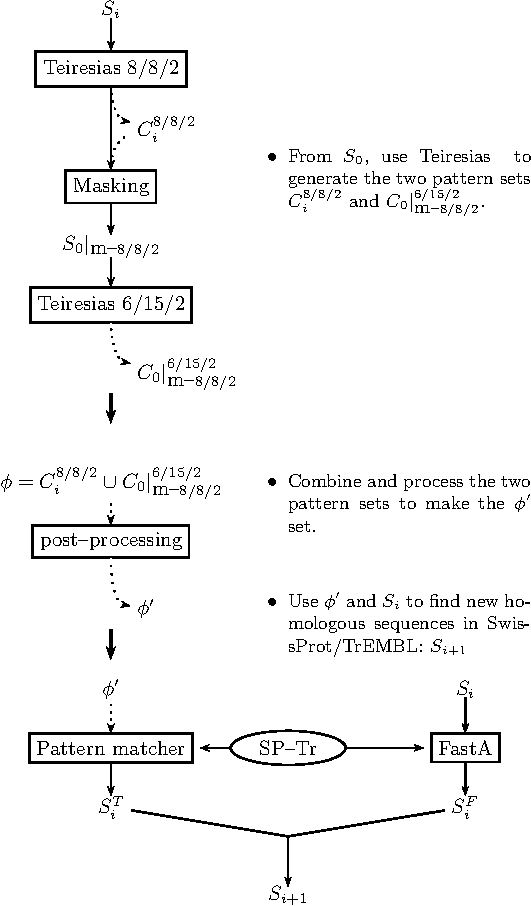
\includegraphics{Body/Images-chap2/bootstrap.pdf}
        \caption[Schematic of the bootstrapping method.]{
            A schematic of the bootstrapping
            method used to collect
            antimicrobial sequences from \sptr
            .  On the left, using \Teiresias,
            we computed an 8/8/2 grammar set
            ($C_i^{8/2/2}$) from the initial
            set of sequences, $S_0$.  These
            grammars were masked from $S_0$
            to make $S_0\mid_{\textrm{m--}8/8/2}$,
            from which the 6/15/2 grammar set,
            $C_0\mid_{\textrm{m--}8/2/2}^{6/15/2}$,
            was found using \Teiresias~ again.
            The two grammar sets were combined
            and processed (see Appendix)
            to make $\phi'$.  This final
            grammar set was used to find more
            antimicrobial sequences in \sptr.
            On the right side of the schematic,
            sequences from $S_0$ were aligned
            against \sptr~ to find new
            antimicrobial sequences.
        }
        \label{fig:bootstrapping}
        \end{figure}


        \subsubsection{Seeding the peptide database
            through similarity searching}
            Starting with our initial
            database of sequences ($S_0$ in
            Figure~\ref{fig:bootstrapping})
            from \sptr~ and \amsdb, we aligned
            each sequence in $S_0$ against
            the entire \sptr~ database.  If a
            sequence in \sptr~ aligned with
            a sequence from $S_0$ with 80\%
            or greater pair--wise identity
            over the length of both sequences,
            the new sequence was marked as a
            possible antimicrobial peptide.
            Of the marked sequences,
            we selected those that were
            from eukaryotic organisms and
            had literature evidence of
            antimicrobial activity.  These
            sequences are shown as $S_0^F$ in
            Figure~\ref{fig:bootstrapping},
            meaning sequences found using
            \Fasta~ in the first iteration.

        \subsubsection{Seeding the peptide
            database through use of grammar
            discovery} In the second stage
            of our bootstrapping method,
            we used \Teiresias~ to find
            grammars that could be used
            to search for antimicrobial
            sequences in \sptr.  As shown in
            Figure~\ref{fig:bootstrapping},
            from the $S_0$ sequence
            set, we derived two separate
            grammar sets ( $C_i^{8/2/2}$ and
            $C_0\mid_{\textrm{m--}8/2/2}^{6/15/2}$),
            which we combined together.  This
            combined set, $\phi$, was processed
            (a detailed description of this
            processing is in the appendix)
            to increase the selectivity and
            sensitivity of the grammars for
            antimicrobial peptide sequences.
            Finally, in each sequence from
            \sptr, we searched for instances
            of grammars from $\phi'$.  If 80\%
            of the amino acids in a peptide
            from \sptr~ were contained within
            instances of grammars from $\phi'$
            the peptide was marked.  Of the
            marked sequences, we selected those
            sequences that were from eukaryotic
            organisms and had literature
            evidence of antimicrobial activity,
            calling these sequences $S_0^T$.

        \subsubsection{Iterating the bootstrapping
            method} The new antimicrobial
            peptides found using \Fasta~ and
            \Teiresias, $S_0^F$ and $S_0^T$
            respectively, were added to the
            initial database, $S_0$, to make
            $S_1$.  Next, a bootstrapping
            method was repeated on the $S_1$
            sequence set to make larger and
            larger sets ($S_2$, $S_3$,\dots)
            until no more antimicrobial
            peptides in \sptr~ could be found.
        This process is shown in Figure~\ref{fig:bootstrapping} and detailed below.
        \begin{enumerate}
            \item \textbf{Finding Highly Conserved grammars}\newline
                First we found all the highly conserved (8/8/2) grammars
                in $S_0$.  These grammars are substrings
                in $S_0$ that are repeated exactly, that is, grammars
                without any wild--cards or bracketed expressions.  Let
                these grammars be called $C_0^{8/2/2}$, meaning
                8/8/2 grammars from the first iteration.  In
                order to simplify the grammar discovery process
                for the next step, the sequence set $S_0$ was
                masked
                \footnote{``Masking'' is described in detail
                    in Rigoutsos and others~\cite{rigoutsos1999dictionary}.  In brief,
                    by masking a grammar, we tag each instance of a grammar
                    except for the instance in the longest sequence in
                    which the grammar is found.  Tagged regions are
                    then excluded from further grammar discovery processes.  }
                with the  $C_0\mid^{8/2/2}$ grammars
                to make the $S_0\mid_{\textrm{m--}8/8/2}$ sequence set.
            \item \textbf{Finding Loosely Conserved grammars}\newline
                Using the $S_0\mid_{\textrm{m--}8/8/2}$ sequences, we
                found all 8/15/2 grammars, which we will call
                $C_0\mid_{\textrm{m--}8/2/2}^{6/15/2}$.
                These grammars are more loosely conserved than the $C_0^{8/2/2}$
                grammars and are typically greater in number.
            \item \textbf{Post--Processing the grammars}\newline
                Let the union of the two grammar sets computed
                above be  $\phi_0 = C_0^{8/2/2} \cup C_0\mid_{\textrm{m--}8/2/2}^{6/15/2}$.
                We would like to match grammars in $\phi_0$ against \sptr~ to find
                any remaining unknown antimicrobial sequences.  But, to gain greater
                specificity and sensitivity, we first processed the grammars in
                $\phi_0$ to a make a grammar set $\phi'0$.

                \begin{enumerate}
                    \item
                        For every grammar in $\phi_0$, we de--referenced
                        each wild--card character that could be expressed as a
                        bracketed expression with no greater than four characters.
                        That is, in the grammar ``\texttt{K.T}'', the ``\texttt{.}''
                        might be replaced with ``\texttt{[AG]}'' if, for each
                        instance of ``\texttt{K.T}'', only ``\texttt{A}'' and
                        ``\texttt{G}'' are found in the wild--card position.  If
                        more than four characters were needed in the bracketed
                        expression, we left the wild--card character instead.

                    \item  For each of the altered grammars in $\phi_0$ we decomposed
                        the grammar into a set of smaller, redundant grammars
                        by using a sliding window of ten non--wild--card characters.  So, a
                        grammar such as ``\texttt{[FWY]FK.[GQ][KRQ]CPDAY}''
                        would be decomposed into three distinct grammars:
                        ``\texttt{S[RKM][FWY]FK.[GQ][KRQ]CPD}'', ``\texttt{[RKM][FWY]FK.[GQ][KRQ]CPDA}'',
                         and ``\texttt{S[RKM][FWY]FK.[GQ][KRQ]CPDAY}'', each ten non--wild--card
                        amino acids in length.

                    \item  From this new, redundant $\phi_0$ we kept only those grammars that
                        were statistically significant.  These are grammars that have a
                        log--odds probability less than or equal to $-30$.

                \end{enumerate}
                Let these the processed $\phi_0$ grammar set be called $\phi'_0$.
        \end{enumerate}
            The final sequence set, from
            the last iteration, became our
            database of known antimicrobial
            peptide sequences and the final
            $\phi'$ became our antimicrobial
            grammar database.


    \subsection{Antimicrobial sequence and grammar databases}

        The initial database of antimicrobial peptides collected from \amsdb~ and \sptr~ contained
        a total of 836 sequences.
        Starting with these sequences, the bootstrapping method
        described previously went through 3 iterations until no more sequences were found
        in \sptr.  The last sequence set, $S_3$, which contained a total of 931 sequences,
        was used as our antimicrobial sequence
        database and is available on--line at \url{http://cbcsrv.watson.ibm.com/Tspd.html}.
        The final grammar set ($\phi'$
        from the last bootstrapping iteration) contained a total of 241,642 grammars
        covering the sequence space of the final sequence database.

        \begin{figure}[ptb]
        \centering
        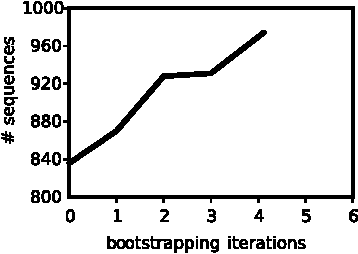
\includegraphics{Body/Images-chap2/growth.pdf}
        \caption[Graph of the progress of the bootstrapping method.]{
            A plot of the progress of the bootstrapping method.  The figure
            shows that our antimicrobial sequence database grew from 836 sequences
            to 931 sequences in 3 iterations.
        }
        \label{fig:bootProgress}
        \end{figure}

    \subsection{Annotator design and validation}
    Together, these $\sim$200K grammars describe the ``language'' of the
    AmP sequences.  In this linguistic metaphor, the peptide sequences are
    analogous to sentences and the individual amino acids are analogous to
    the words in a sentence.  Each grammar describes a common arrangement
    of amino acids, similar to popular phrases in English.

    Given an arbitrary sequence of amino acids, it is possible that
    some parts of the sequence are ``matched'' by one or more of the
    grammars in our database.  For example, the white mustard plant
    AmP Afp1 (Genbank accession no.\ P30231) contains the amino acid
    sequence fragment \texttt{CICYFPC}, which matches the grammar
    \texttt{CICY[FVK]PC} from our database.  (As discussed in Section~\vref{section:regex},
    the bracketed expression
    \texttt{[FVK]} indicates that, at the fifth position in the grammar,
    either phenylalanine, valine, or lysine is equally acceptable.)  Based on
    this match, we would say that the Afp1 fragment is ``grammatical.''


        Using the antimicrobial grammar database, we created an on--line tool
        for annotating antimicrobial peptides by determining the degree to which
        a query sequence is grammatical.  (This tool is
        available online at
        \url{http://cbcsrv.watson.ibm.com/Tspd.html}.)
        A user--supplied input sequence is annotated by generating grammar--based alignments
        of the input against sequences in our database of known antimicrobial
        sequences ($S$).  This alignment takes place
        in two distinct steps.  First, we search the input sequence for instances
        of grammars from the antimicrobial grammar database (the final $\phi'$).
        Second, for each contiguous stretch of shared grammars between the input
        sequence and a sequence from $S$, an alignment is produced.  Figure~\ref{fig:alignment}
        show a schematic of the alignment process.


        \begin{figure}[ptb]
        \centering
        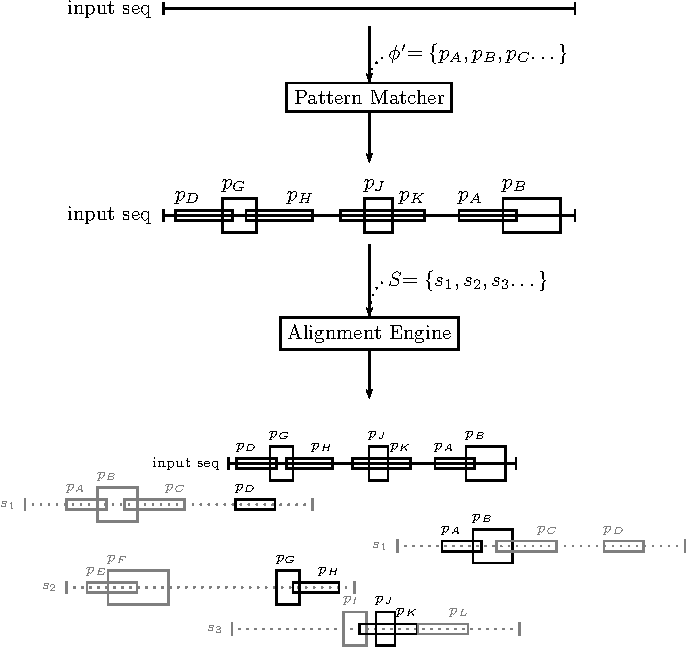
\includegraphics{Body/Images-chap2/alignment.pdf}
        \caption[Schematic of the grammar--based alignment method]{
            A schematic of our grammar--based alignment method.  In the figure, a user--supplied
            input sequence is searched for instances of grammars ($p_A,p_B,p_C$\ldots) that occur
            in the set of known antimicrobial sequences ($S$).  Grammars that occur in both the
            input sequence and sequences in  $S$ are then used to create alignments.  As indicated in
            the figure, the input sequence shows homology to $s_1$ in two distinct regions, so
            both possible alignments are shown.  See
            Figure~\vref{fig:ampAlign} for an example of how these
            grammar--based alignments appear in practice.
        }
        \label{fig:alignment}
        \end{figure}

        \begin{sidewaysfigure}[ptb]
        \centering
        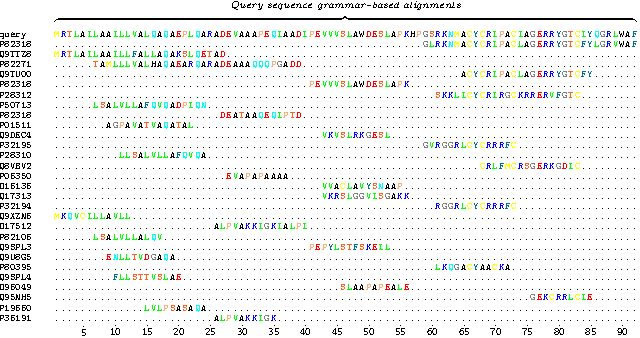
\includegraphics[width=\textheight]{Body/Images-chap2/amp-align.pdf}
        \caption[Example results of the grammar--based alignment method]{
            Example results of the grammar--based alignment method.
            The figure shows the annotation of a query sequence
            after it has been searched exhaustively for grammars in
            our database of $\sim$200K grammars describing the
            ``language'' of AmPs.  This alignment was generated
            using the methodology detailed in
            Figure~\vref{fig:alignment}.  Each of the sequences
            below the query is an AmP sequence from our database,
            $S$.  The sequences are aligned against the query
            because they share grammars in common at those
            particular loci.  However, different sequences may share
            very in degrees of conservation, even if they have the
            same grammar.  For example, see Figure~\vref{table:cons}.
        }
        \label{fig:ampAlign}
        \end{sidewaysfigure}

        \begin{sidewaystable}[ptbh]
    \caption[Motif conservation]{Motif conservation for the query shown in Figure and the motif \texttt{L[VQH][ALV][KLPQ][AS][EAF][APQS][ALRV]QA}.}
	\label{table:cons}
	\centering 
    \begin{tabular}{lllll} \hline\hline
QUERY		&	\texttt{LQAQAEPLQA}\\	\hline
P17534	&	\texttt{LVLLAFQVQA}	&	40.00\%	&	Cryptdin-related protein 4C-1	&	  Mus musculus (Mouse). \\
P19660	&	\texttt{LVLPSASAQA}	&	30.00\%	&	Bactenecin 5 precursor (BAC5)	&	  Bos taurus (Bovine). \\
P19661	&	\texttt{LVLPSASAQA}	&	30.00\%	&	Bactenecin 7 precursor (BAC7)	&	  Bos taurus (Bovine). \\
P28309	&	\texttt{LVLLSFQVQA}	&	30.00\%	&	Cryptdin-2 precursor	&	  Mus musculus (Mouse). \\
P28310	&	\texttt{LVLLAFQVQA}	&	40.00\%	&	Cryptdin-3 precursor	&	  Mus musculus (Mouse). \\
P28311	&	\texttt{LVLLAFQVQA}	&	40.00\%	&	Cryptdin-4 precursor	&	  Mus musculus (Mouse). \\
P28312	&	\texttt{LVLLAFQVQA}	&	40.00\%	&	Cryptdin-5 precursor	&	  Mus musculus (Mouse). \\
P32195	&	\texttt{LVVPSASAQA}	&	30.00\%	&	Protegrin 2 precursor (PG-2)	&	  Sus scrofa (Pig). \\
P33046	&	\texttt{LVVPSASAQA}	&	30.00\%	&	Indolicidin precursor	&	  Bos taurus (Bovine). \\
P49930	&	\texttt{LVVPSASAQA}	&	30.00\%	&	Antibacterial peptide PMAP-23	&	  Sus scrofa (Pig). \\
P49931	&	\texttt{LVVPSASAQA}	&	30.00\%	&	Antibacterial peptide PMAP-36	&	  Sus scrofa (Pig). \\
P49932	&	\texttt{LVVPSASAQA}	&	30.00\%	&	Antibacterial peptide PMAP-37	&	  Sus scrofa (Pig). \\
P50704	&	\texttt{LVLLAFQVQA}	&	40.00\%	&	Cryptdin-6/12 precursor	&	  Mus musculus (Mouse). \\
P50705	&	\texttt{LVLLAFQVQA}	&	40.00\%	&	Cryptdin-7 precursor	&	  Mus musculus (Mouse). \\
P50707	&	\texttt{LVLLAFQVQA}	&	40.00\%	&	Cryptdin-9 precursor	&	  Mus musculus (Mouse). \\
P50708	&	\texttt{LVLLAFQVQA}	&	40.00\%	&	Cryptdin-10 precursor (Fragmen	&	  Mus musculus (Mouse). \\
P50711	&	\texttt{LVLLAFQVQA}	&	40.00\%	&	Cryptdin-13 precursor	&	  Mus musculus (Mouse). \\
P50712	&	\texttt{LVLLAFQVQA}	&	40.00\%	&	Cryptdin-14 precursor (Fragmen	&	  Mus musculus (Mouse). \\
P50713	&	\texttt{LVLLAFQVQA}	&	40.00\%	&	Cryptdin-15 precursor	&	  Mus musculus (Mouse). \\
P50714	&	\texttt{LVLLAFQVQA}	&	40.00\%	&	Cryptdin-16 precursor	&	  Mus musculus (Mouse). \\
P51525	&	\texttt{LVVPSASAQA}	&	30.00\%	&	Prophenin-2 precursor (PF-2) (	&	  Sus scrofa (Pig). \\
P82270	&	\texttt{LHAQAEARQA}	&	70.00\%	&	Theta defensin-1, subunit A pr	&	  Macaca mulatta (Rhesus macaque). \\
P82271	&	\texttt{LHAQAEARQA}	&	70.00\%	&	Theta defensin-1, subunit B pr	&	  Macaca mulatta (Rhesus macaque). \\
P82318	&	\texttt{LQAQAEPLQA}	&	100.00\%	&	Neutrophil defensins 1, 3 and	&	  Macaca mulatta (Rhesus macaque). \\
Q01524	&	\texttt{LQAKAEPLQA}	&	90.00\%	&	Defensin 6 precursor (Defensin	&	  Homo sapiens (Human). 
	\\ \hline\hline
	\end{tabular}
	\end{sidewaystable}


    Since it is possible that, for an arbitrary sequence, only a portion
    of the sequence is matched by one of our grammars, we developed a
    heuristic metric $Z$, which is the degree to which a query sequence
    is grammatical.  To calculate $Z$, we assign a local score along the
    backbone of a query sequence that is equal to the number of grammars,
    or fractions of grammars with at least 10 amino acids, that have
    matches over the length of the query sequence.  The total score for
    the sequence, $Z$, is the fraction of the sequence's length that
    is covered by at least one grammar (see Figure~1\ref{fig:space}).
    For example, a hypothetical sequence \texttt{LFLTAIDRYIAAA} ---
    which is matched by \texttt{LFLTAI[ID][TR][VY]I}, but no other
    grammars in our database --- would get a score of 10/13 since the
    first 10 positions in the sequence are covered by the match.

    In order to annotate and design synthetic AmPs, we created a software tool to
    calculate the score $Z$ for a query sequence and to classify the
    sequence as either likely to have antimicrobial activity --- if its
    $Z$--score is above a certain threshold --- or not.  To determine
    this threshold, we trained the tool on a subset of sequences from our
    AmP database as follows.  We randomly selected $90\%$ of the natural
    AmP sequences and generated a Teiresias grammar set, using the same
    Teiresias parameters that were used to generate our $\sim$200K grammar
    set.  This smaller grammar set was used by our software to classify
    the remaining $10\%$ of our AmP database, which was hidden among
    $10\%$ of the non--AmP sequences from Swiss--Prot/TrEMBL ($\sim$78K
    sequences).  This experiment was repeated 300 times, with different
    random sets, to determine the best $Z$--score.  We found that, at
    an $Z$--score threshold of 0.73, the software tool will correctly
    classify both the AmP and non--AmP sequences with $99.95$\% accuracy.


\section{Preliminary strategy for the design of novel
AmPs}\label{section:preliminary}

    \subsection{Sequence design}
    As I showed in the previous section, the $Z$--score annotation
    metric is both sensitive and selective for existing AmPs.
    We hypothesized that this metric could be used equally well to
    design unnatural sequences that would have antimicrobial
    activity.  In this section, I describe our preliminary strategy
    for designing these novel, unnatural sequences.
    \textit{Notably, the experimental data presented
    in this section were later discovered to not be
    reproducible due to experimental complications. See
    Section~\vref{section:fake}.  The data are presented
    here for the insight they lend to our more focused,
    and successful, strategy for designing AmPs, which is
    described in Section~\vref{section:focused}.}

    Based on the annotation results described in the previous
    section,
    we ran a computer simulation to create novel amino acid sequences
    with high $Z$--scores, but with minimal homology to natural AmPs.
    This simulation, shown schematically in Figure~\vref{fig:evolution},
    used the $Z$--score as a fitness function for the \emph{in
    silico} directed evolution of these novel sequences.  To begin,
    we created a randomized database of 100K progenitor sequences
    of uniform length with the same amino acid composition (i.e.,
    the same percentage of each amino acid type) as our AmP database.
    Each of these sequences was allowed to have 4 mutated ``children,''
    which were each 100 PAM (point accepted mutations) evolutionary
    units away from the parent.  (The implied rates of mutation from
    the Blosum--50 matrix were used to make the mutations at the amino
    acid level~\cite{henikoff1992aminoacid}.)  These children, each
    of which differed from their parent sequence by at least one amino
    acid, were added to the total population of sequences.  In order to
    avoid generating sequences that were similar to natural AmPs, the
    population was purged of any sequences that had 6 or more consecutive
    amino acids in common with any natural AmP sequence.  Finally,
    the remaining sequences were scored using our annotation software.
    From the population, the sequences with the top 100 $Z$--scores
    were propagated to the following round, and the entire process was
    repeated.


        \begin{figure}
        \centering
        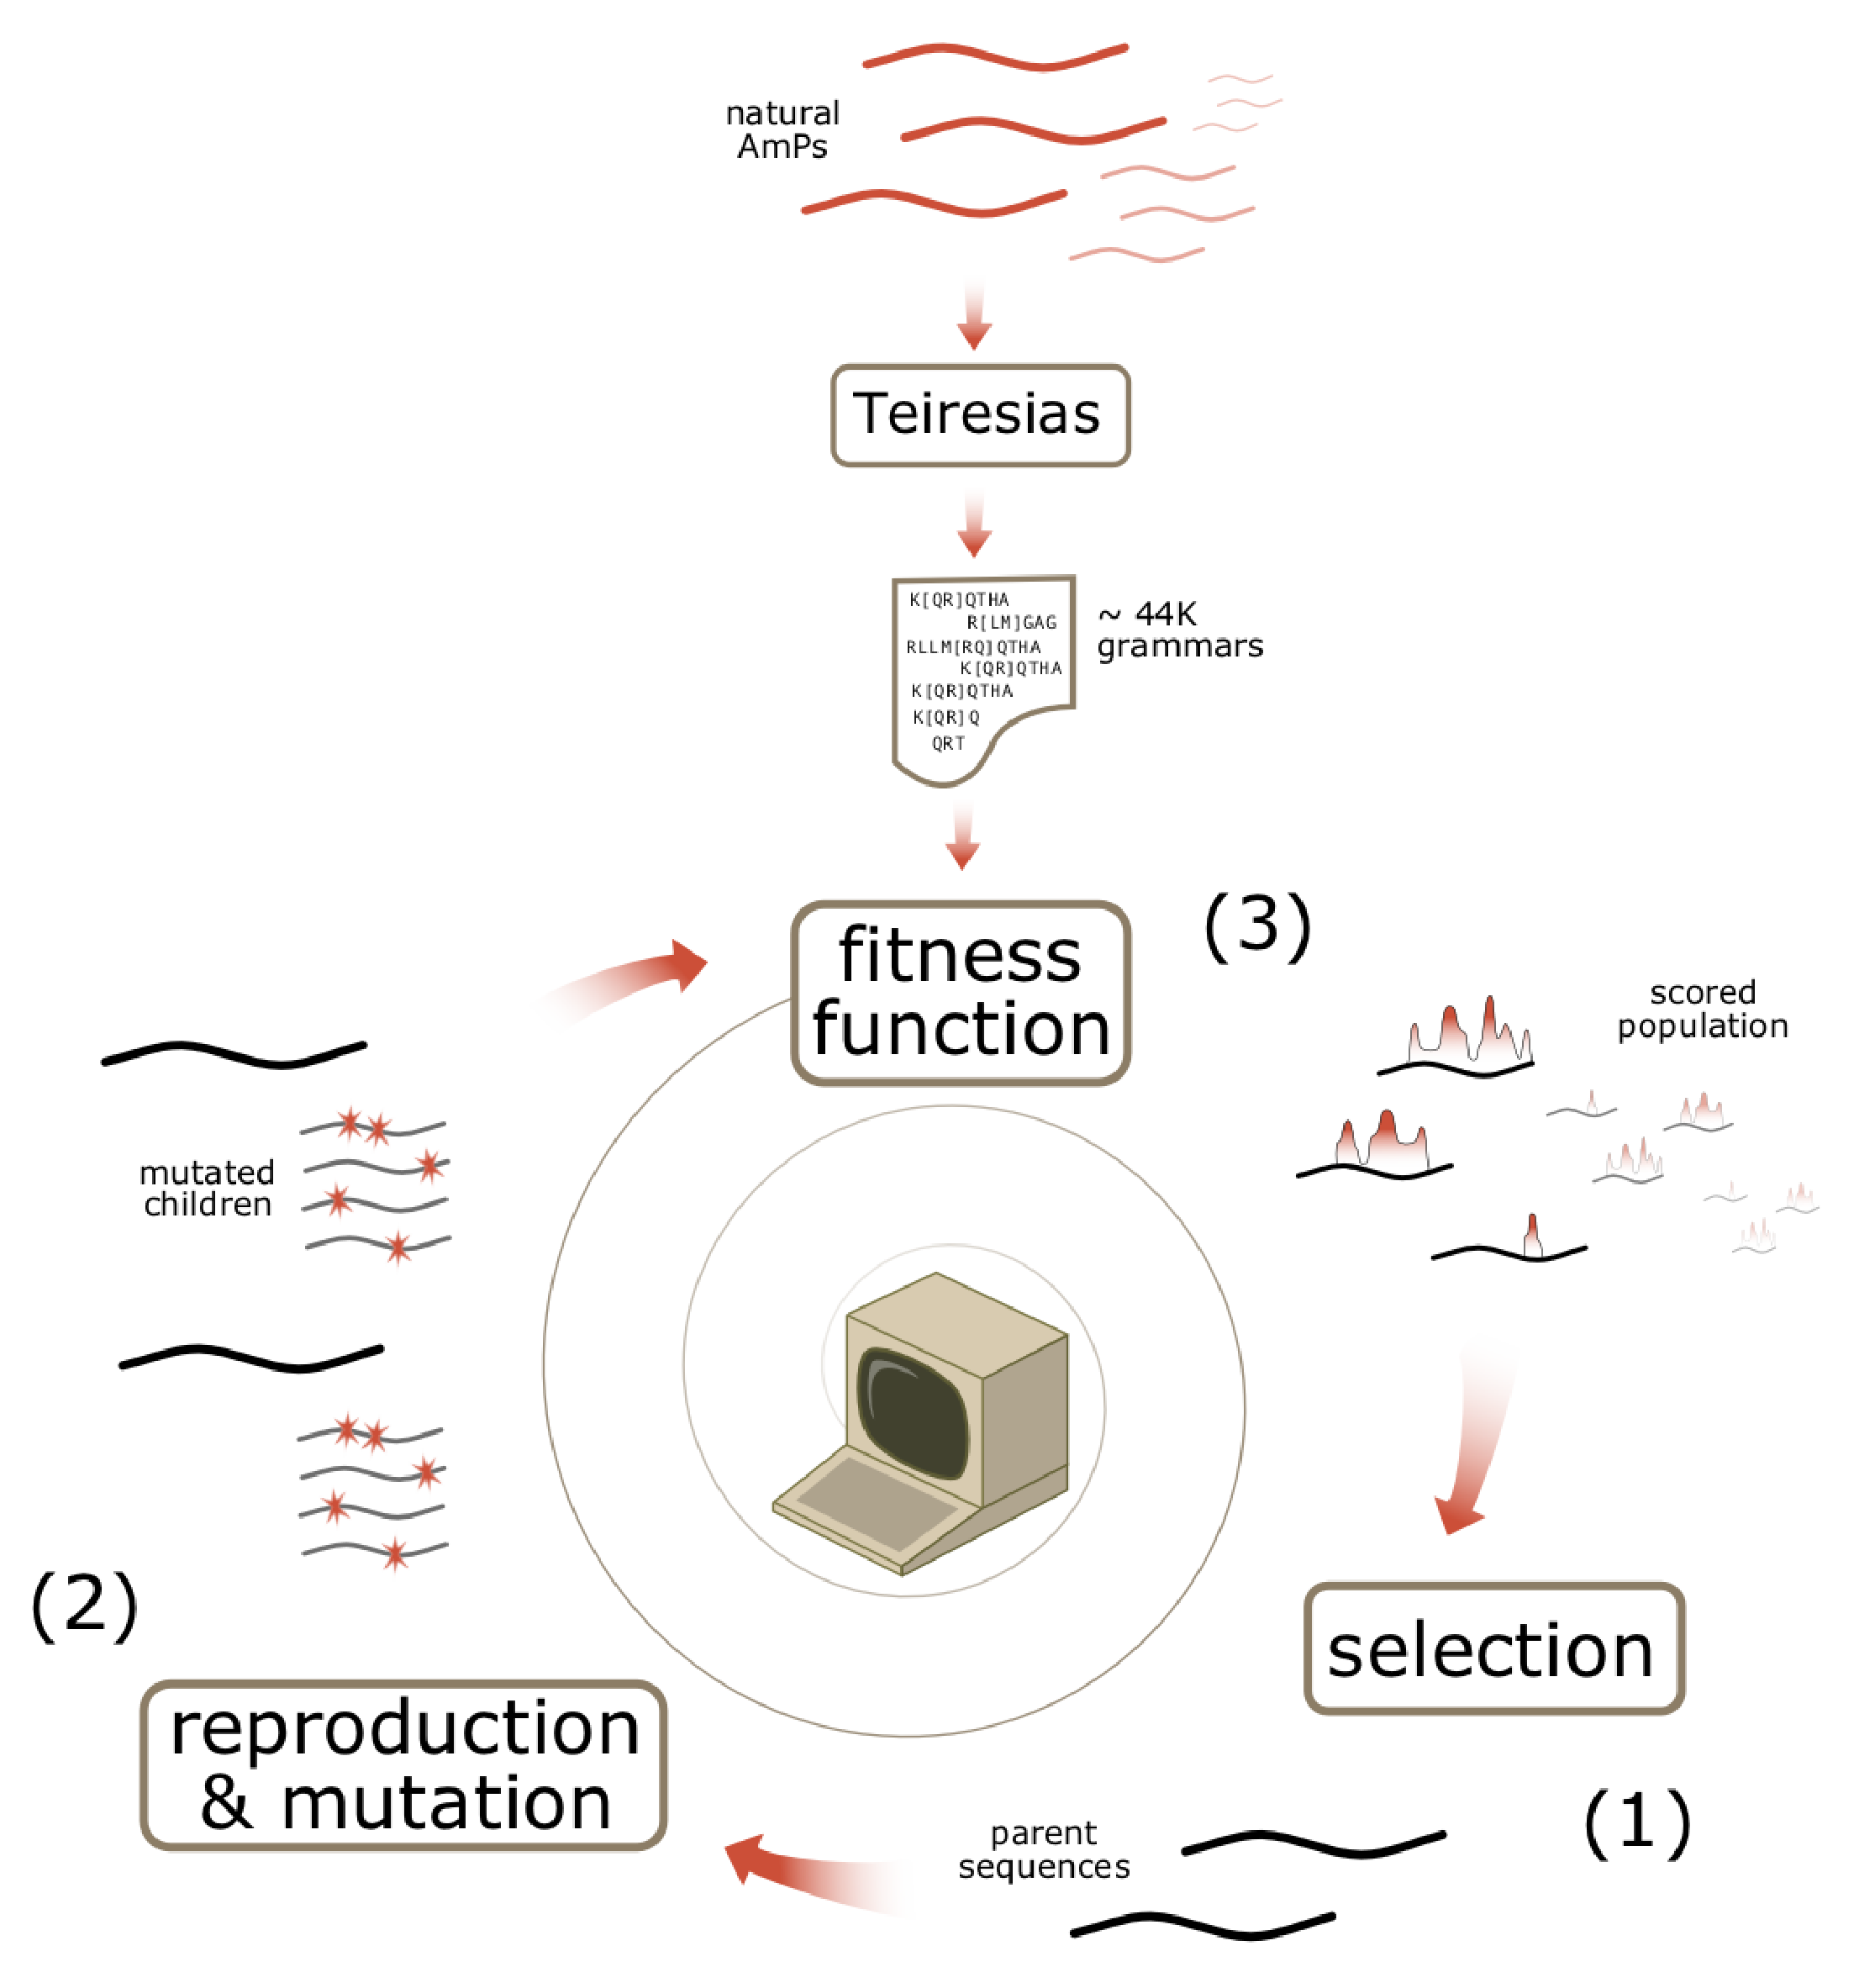
\includegraphics[width=\textwidth]{Body/Images-chap2/evolution.pdf}
        \caption[Directed evolution]{ A schematic of the \emph{in
        silico} directed evolution strategy.  Position (1)
        shows the starting point: the database of 100K parental
        sequences.  Each of these sequences has 4 mutated
        children (2) and the entire population is scored using the
        $Z$--score and our database of grammars from natural AmPs.
        From the scored population (3), the top 100 sequences
        are chosen and become the parental sequences for the
        next iteration.  In addition to the directed evolution
        simulation, we considered other methods for generating
        sequences with high $Z$--scores.  However, we chose this
        approach because it naturally allows for sequences of
        arbitrary length and the possibility that grammars may
        overlap in the designed amino acid sequences.}%
        \label{fig:evolution}
        \end{figure}

    Using the strategy described above, we allowed many populations
    of sequences to evolve, each with a different sequence length,
    which remained constant during the simulation.  We stopped each
    simulation after $3,000$ rounds of mutation and selection, by which
    point we found that populations of small sequence length would have
    converged to $S=1$.  For longer length populations, all the sequences
    typically reached at least $S=0.73$ and all tended to be closely
    related to each other.  We chose three sequences of lengths 20, 31,
    and 63 amino acids to test experimentally for antimicrobial activity:
    sequences synth--1, 2, and 3 in Table~\vref{table:peptides}.



\begin{sidewaystable}[ptbh]
    \caption[The preliminary design synthetic antimicrobial peptides used in this study]{The preliminary design synthetic antimicrobial peptides used in this study
	For each synthetic AmP we also designed two sequences
	(``negative'' a and b), which have the same amino acid
	composition as the synthetic peptide but have an $S$--score
	of zero.  The table also shows statistics relavant to
	AmPs, which were calculated using the EMBOSS software
	package\cite{rice2000emboss}.  Note that synth--3 has only
	one negative version.  Also, the peptides synth--1, 2, and 3
	were the \emph{only} peptides designed using our grammatical
	approach that were synthesized and tested experimentally.
        }\label{table:peptides} \begin{center} 
    \begin{tabular}{lccccl} \hline \hline
	Peptide &  S & Size & Charge & pI & Sequence\\ \hline
	\textbf{synth--1:} &  & 20 & 4.5 & 11.92\\
	~~~synth--1 & 1 &  &  &  & {\footnotesize \ttfamily NKVKKPLTGAHRLLFTFLFV} \\
	~~~negative--1a & 0 &  &  &  & {\footnotesize \ttfamily VVLKLLFFKFNLPHKTRTAG} \\
	~~~negative--1b & 0 &  &  &  & {\footnotesize \ttfamily LVLTFLFATPKLNGRVKKFH} \\
	\textbf{synth--2:} &  & 31 & 10.0 & 11.28 \\
	~~~synth--2  & 1 &  &  &   & {\footnotesize \ttfamily MKKIKKEAGKNILKLAPKEVAAKKSKKSPTK} \\
	~~~negative--2a  & 0 &  &  &   & {\footnotesize \ttfamily PAAGESKVKANKKKAKILPTMKLKKEIKKKS} \\
	~~~negative--2b  & 0 &  &  & 	& {\footnotesize \ttfamily SEASLKAKIKKIAMKKVTKGKAKNKPKLPEK} \\
	\textbf{synth--3:}&  & 63 & 3.0 & 10.41\\
	~~~synth--3 & 0.92 &  &  &   & {\footnotesize \ttfamily MKDKNSTGPLLSALLLAVTAGGSPVAAAPWNPFAAILKAALQIAGAAEPKEVTAKKGPTKADA}\\
	~~~negative--3a & 0 &  &  &  & {\footnotesize \ttfamily GWAGLVAETAIADKMSLKAAGEPPNQNDGAVLKTPPKAAASAKPLGAAKTLAFISPVTLALAK}\\
	%~~~negative--3b & 0 & 63 & 3.0 & 10.41  & {\footnotesize \ttfamily AAKGVAAAPEANALSAWTTPMGLGGSIGFDKPPKKALKNKLTPAAVKSVLLPALATIAQEDAA}
	\\ \hline\hline
    \end{tabular} \end{center}

 \end{sidewaystable}




    Using NCBI Blast~\cite{altschul1997gapped} (blastp) with the default
    parameters, we compared these sequences to the entire NCBI NR
    sequence database.  The Blast results showed that none of the three
    sequences has significant homology to \emph{any} known protein
    (E--value $\leq$10), including the naturally--occurring AmPs.
    (More extensive similarity searching using PSI--Blast and E--value
    thresholds up to $\leq$50 also failed to detect similarity to any
    natural AmPs.)  This is possible because each grammar can be written
    in a large number of ways.  For example, the 10--residue grammar
    \texttt{[LV][GA]K[TN][FL]AGHML} occurs in 3 natural AmPs, but there
    are 16 possible 10--residue sequences that match this grammar.
    Since our sequences are built from tiled grammars, the synthetic
    sequences can quickly deviate from the naturally populated sequence
    space such that it is impossible to detect similarity using sequence
    alignment tools (see Figure~\vref{fig:space}).



        \begin{figure}
        \centering
        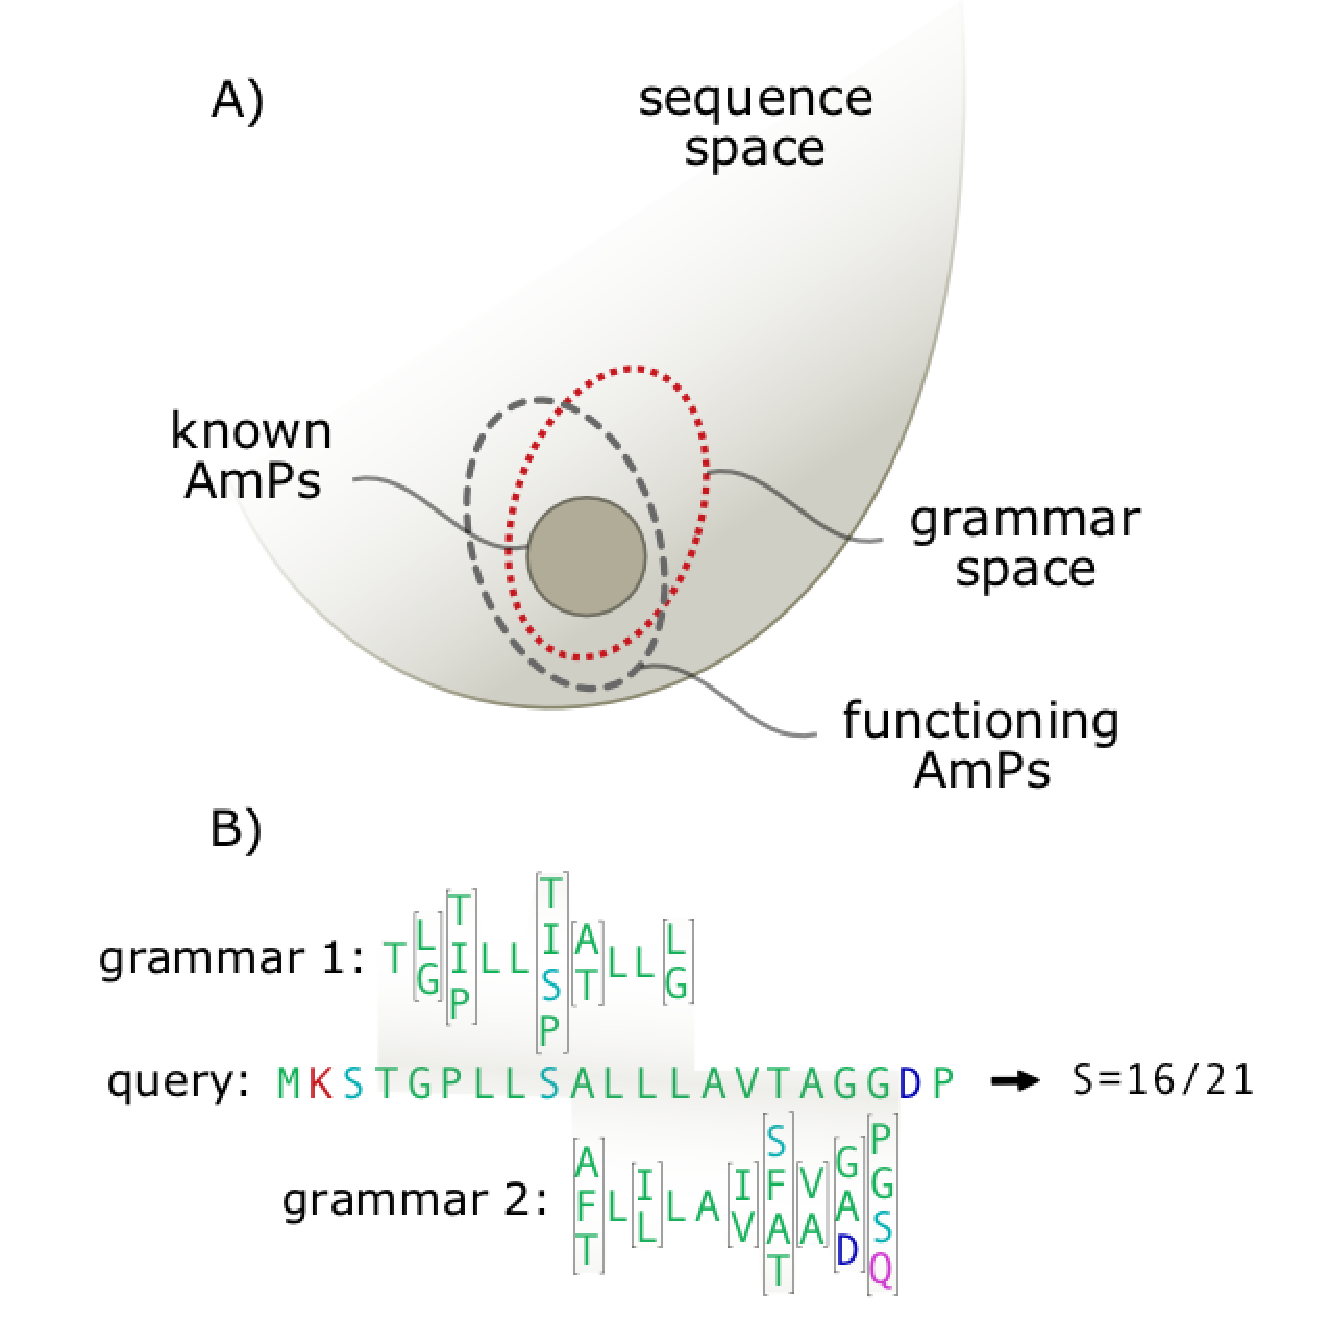
\includegraphics[width=0.75\textwidth]{Body/Images-chap2/space.pdf}
        \caption[Design space]{ The AmP design space.
        Part A shows the sequence space surrounding the set of
        natural AmPs.  The ``sequence space'' is the combinatorially
        large set of all possible sequences.  Even for a 20--residue
        peptide like synth--1 (see Table~\ref{table:peptides})
        this space is huge: $20^{20}\approx 10^{26}$ sequences.
        (For comparison, there are about $10^{22}$ stars in the known
        universe.)  Our linguistic model focuses the search space to
        the ``grammar space,'' but allows a deviation from natural
        AmP sequences.  This allows us to design peptides that show
        no significant homology to any naturally occurring sequences,
        but have the desired function.  Part B shows a subsequence
        of the synth--2 peptide.  Above and below the subsequence
        are grammars that match the sequence in a tiled arrangement.
        For each bracketed expression, any of the amino acids listed
        in the bracket will suffice.}
        \label{fig:space}
    \end{figure}


    For each of the three synthetic peptides, we also designed a
    set of shuffled sequences, which we hypothesized would have no
    antimicrobial activity.  These ``negative'' peptides are shown along
    with the three synthetic peptides in Table~\ref{table:peptides}.
    The negative peptides have the same amino acids as the synthetic
    sequences (and thus, the same molecular weight, charge, and pI);
    however, the order of the amino acids was shuffled so that the
    negative sequences each have an $Z$--score of zero.



\subsection{Peptide synthesis and validation}
    Using an approach described elsewhere~\cite{martemyanov2001cell}, we
    synthesized all 8 of the peptides shown in Table~\ref{table:peptides}.
    For each peptide we created a translation template
    consisting of three parts: green fluorescent protein (GFP) with a
    T7 promoter, an enterokinase recognition site (ERS), and the AmP to
    be tested.  We synthesized the protein--product of each template in
    an \emph{E. coli}--derived \emph{in vitro} translation system
    with continuous exchange~\cite{kim1996semicontinuous}.  The resulting
    peptides were proteolytically cleaved with enterokinase and the yield
    of AmP in the translation mixture was measured via GFP fluorescence
    using a 1:1 molar equivalence between the AmP and GFP concentrations.

    We characterized the antimicrobial activity of each
    synthetic AmP using a broth microdilution assay described
    previously~\cite{amsterdam1996susceptibility}.  The top
    section of Table~\ref{table:results} shows the activities of the
    synthetic peptides against four bacterial species: \emph{Bacillus
    cereus}, \emph{Corynebacterium glutamicum}, \emph{E. coli}, and
    \emph{Citrobacter rodentium}.  (See also Figure~\vref{fig:graph2}.)
    These data suggested that all three synthetic peptides
    had antimicrobial activity.  Furthermore, none of the negative,
    ``un--grammatical'' sequences had any activity.  Thus, it appeared that the activity
    of the designed peptides was not an artifact of molecular weight,
    charge, or pI\@.  Instead, the activity appeared correlated to the $Z$--score,
    suggesting that higher order sequence features are responsible for
    antimicrobial activity.  (\emph{These data were later shown to be
    not reproducible.  Later experiments showed that the
    sequences in Table~\ref{table:results} did not have
    detectable levels of antimicrobial
    activity under a more stringent assay. See Section~\vref{section:fake}.})

    The bottom of Table~\ref{table:results} shows the measured activities of
    synth--1 variants that were synthesized chemically --- the peptides
    were purchased in 70\% minimum purity from Invitrogen (Carlsbad, CA)
    --- instead of by our \emph{in vitro} method.  As shown, the activity
    profiles for these peptides appeared to match their \emph{in vitro}--synthesized
    counterparts, suggesting that the antimicrobial activity was not
    a relic of the translation mixture.  (We also used the chemically
    synthesized copy of synth--1 to validate the size of our \emph{in
    vitro} synthesized copy; see Figure~3\ref{fig:gel}.)  Furthermore,
    we found that luciferase (a luminescent protein with no antimicrobial
    characteristics), when synthesized via our \emph{in vitro} method,
    had no activity.  Thus, we were confident that the translation mixture
    had no innate antimicrobial activity that may have produced spurious
    results.

        \begin{figure}
        \centering
        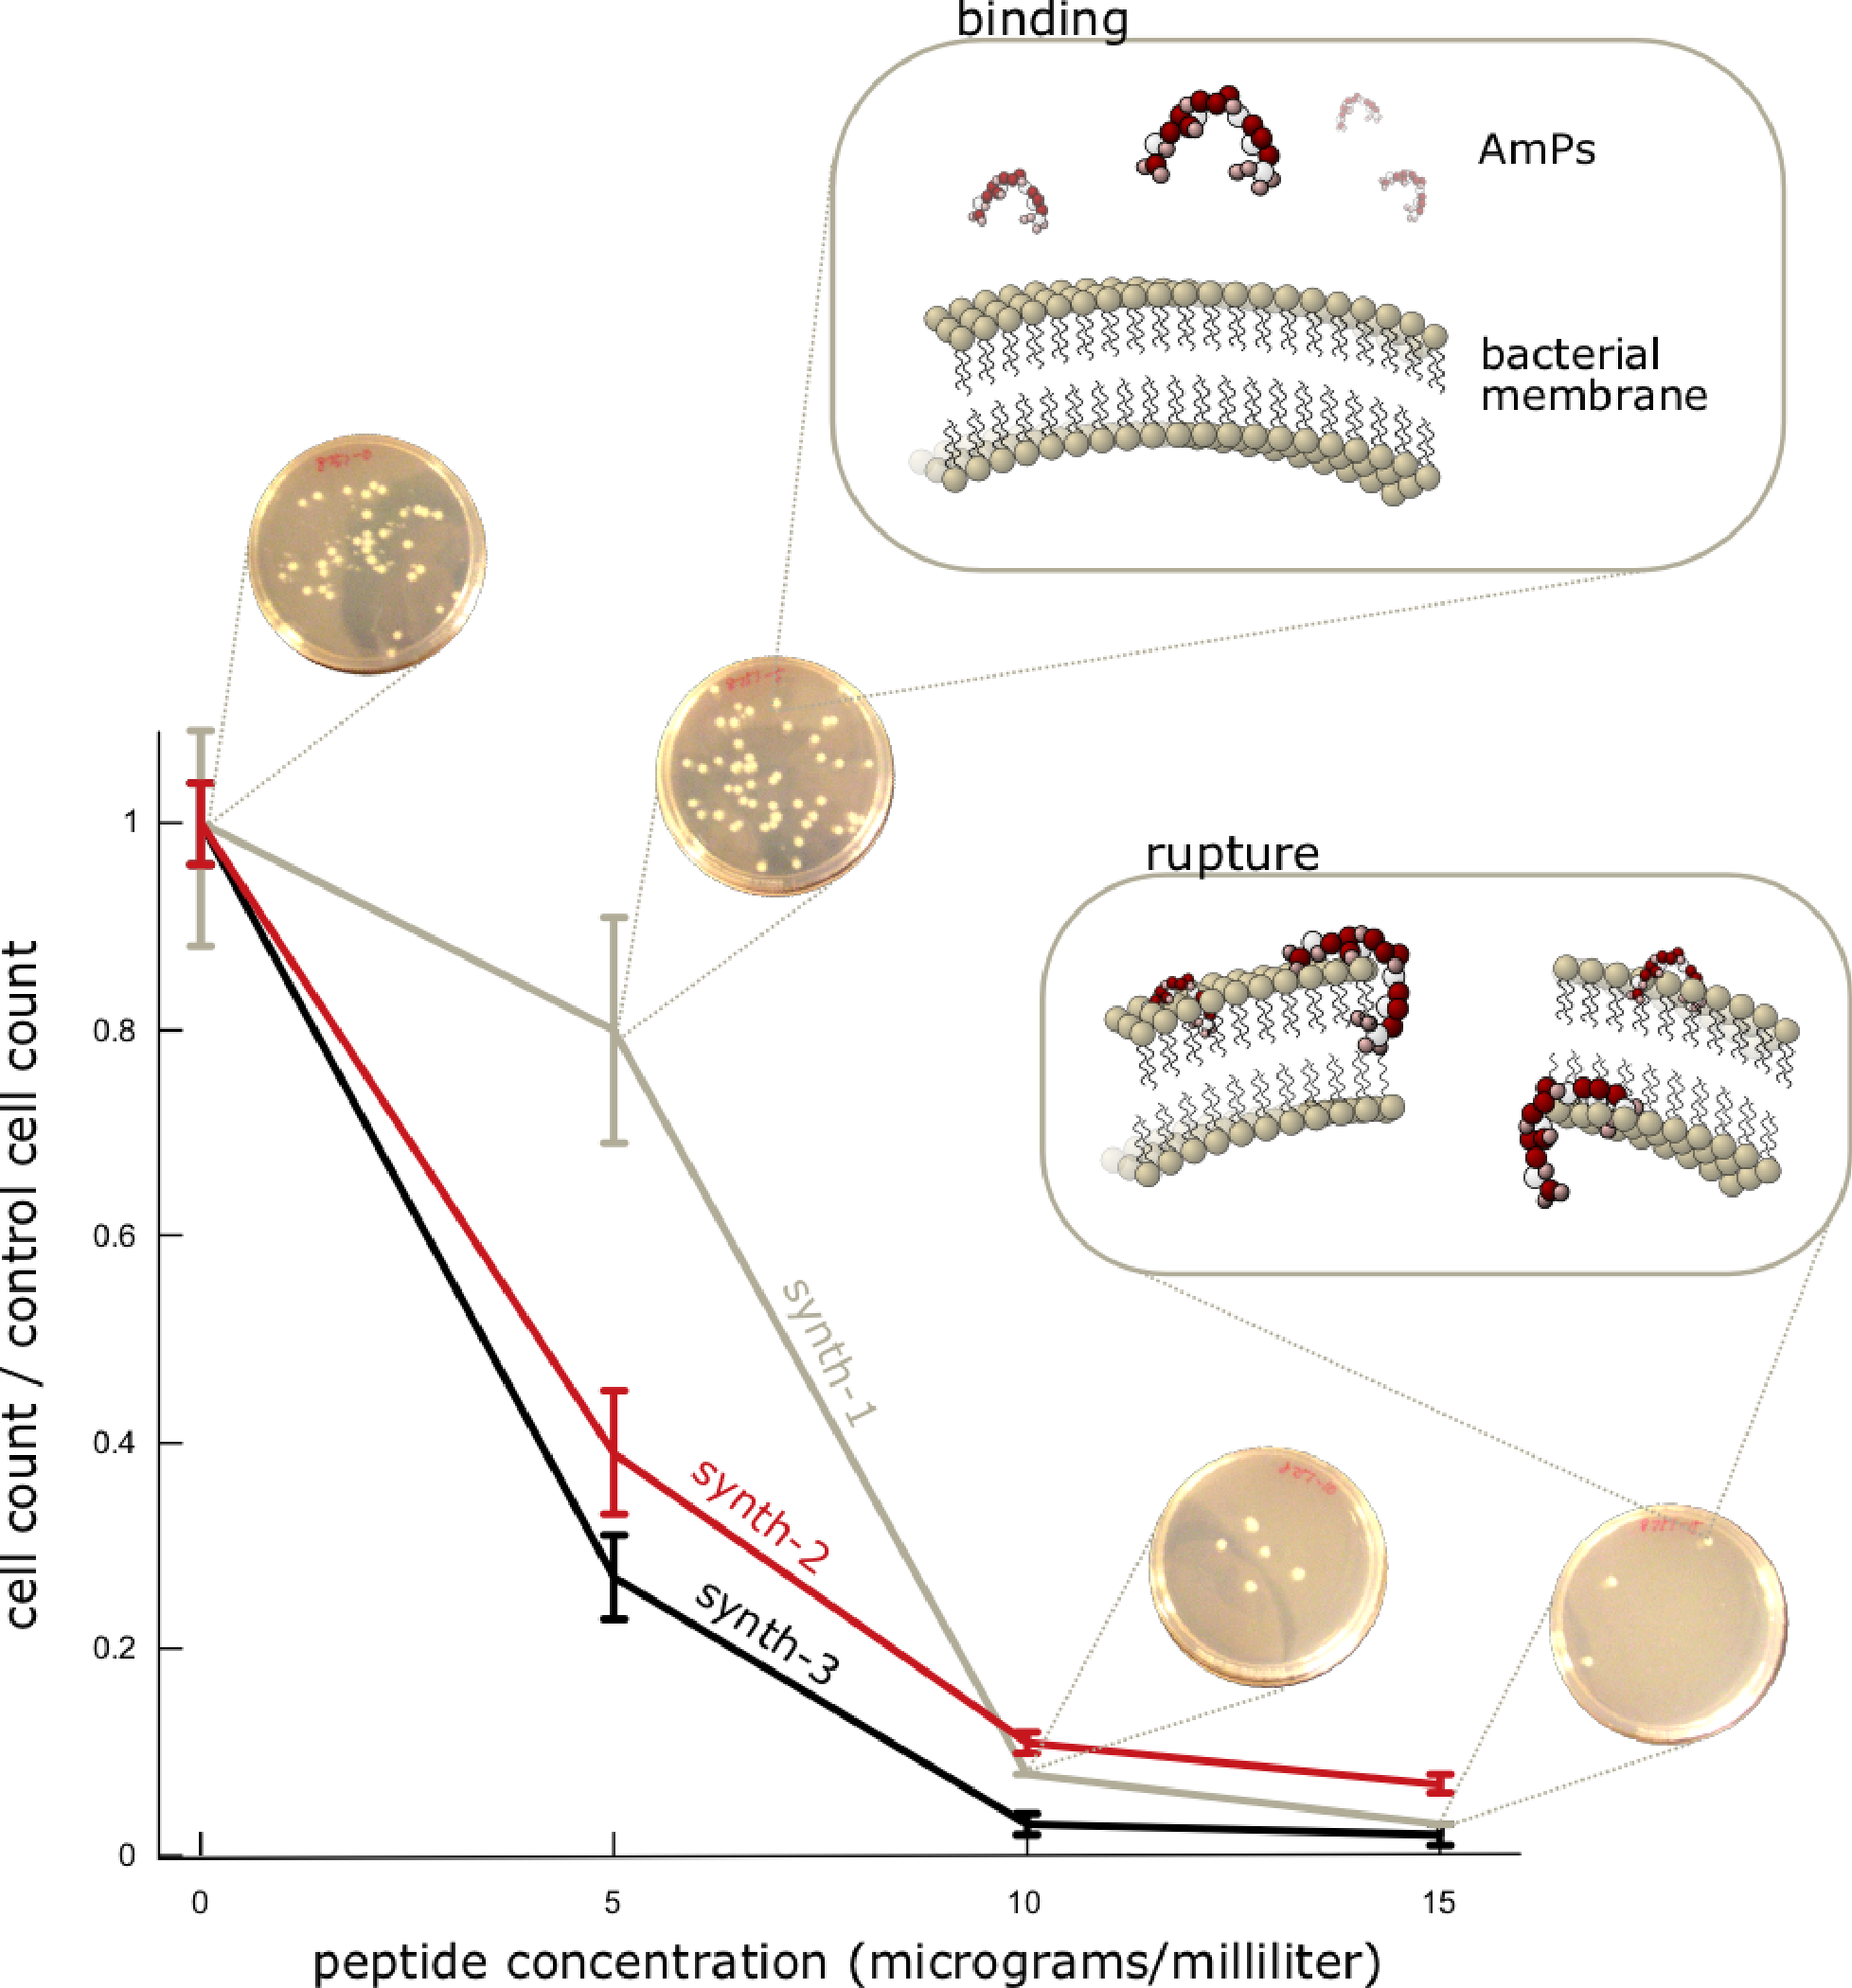
\includegraphics[width=0.95\textwidth]{Body/Images-chap2/detailed-graph.pdf}
        \caption[Antimicrobial peptide action]{Bacteriostatic activity
        of the three synthetic AmPs against \emph{B. cereus}.
        The breakouts show photographs of the colonies, which
        decreased
        in number with increasing peptide concentration.  The inlaid
        schematic shows the generally accepted mechanism of AmP
        action: the electrostatic affinity for the outer--leaflet
        of the bacterial membrane leads to binding and rupture of
        the cell~\cite{shai2002mode}.
        (\emph{These data were later shown to be
    not reproducible.  Later experiments showed that 
    these
    peptides had undetectable levels of antimicrobial
    activity under a more reliable antimicrobial assay. See Section~\vref{section:fake}.})}
        \label{fig:graph2}
    \end{figure}


        \begin{figure}
        \centering
        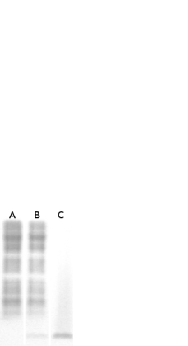
\includegraphics{Body/Images-chap2/control-gel.pdf}
        \caption[Gel picture]{SDS--PAGE gel showing the synth--1
        \emph{in vitro} translation product (lane B).  Lane
        A shows the translation mixture with no peptide and
        lane C shows the *synth--1 peptide, which was produced
        via solid phase synthesis and validated by mass
        spectroscopy.}
        \label{fig:gel}
    \end{figure}



\begin{sidewaystable}[ptbh]
    \caption[Antimicrobial activity of the synthetic peptides against a variety of bacteria]{Antimicrobial activity of the synthetic peptides against a variety of bacteria.
	Each entry in the table shows the relative viability of
	the bacteria: the ratio of the cell count at a particular
	concentration of AmP to the cell count at 0 $\mu$g/mL.  The entries
	in dark gray show high viability (low antimicrobial action) and the
	white entries show low viability (high antimicrobial action).
	The names prepended with a ``*'' are peptides that were chemically
	synthesized rather than produced via \emph{in vitro} translation.
	    }\label{table:results} \begin{center} %\scriptsize
    %\begin{tabular}{lcccc|cccc|cccc|cccc} \hline \hline
    \begin{tabular}{lc@{\extracolsep{0.0mm}}c@{\extracolsep{0.0mm}}c@{\extracolsep{0.0mm}}c@{\extracolsep{2mm}} c@{\extracolsep{0.0mm}}c@{\extracolsep{0.0mm}}c@{\extracolsep{0.0mm}}c@{\extracolsep{2mm}} c@{\extracolsep{0.0mm}}c@{\extracolsep{0.0mm}}c@{\extracolsep{0.0mm}}c@{\extracolsep{2mm}}c@{\extracolsep{0.0mm}}c@{\extracolsep{0.0mm}}c@{\extracolsep{0.0mm}}c@{\extracolsep{0.0mm}}}% \hline \hline
	species $\rightarrow$	
	& \multicolumn{4}{c}{ \underline { \emph{B. subtilis} }}
	& \multicolumn{4}{c}{ \underline {\emph{C. glutamicum} }}
	& \multicolumn{4}{c}{ \underline {\emph{E. coli} }}
	& \multicolumn{4}{c}{ \underline {\emph{C. rodentium} }}\\
	peptide conc. ($\mu$g/mL) $\rightarrow$ & 0 & 5 & 10 & 15
	& 0 & 5 & 10 & 15
	& 0 & 5 & 10 & 15
	& 0 & 5 & 10 & 15\\ %\hline
	\textbf{synth--1:}\\
	%~~synth--1 & 1.00 &  0.80 & 0.08 & 0.03 & 1.00 & 0.73 & 0.21 & 0.15 &  1.00 & 1.02 & 1.00 &   0.93 & 1.00 &  0.99  &  0.97  &  0.98 \\
	%~~negative--1a & 1.00 & 0.96 & 1.01 & 1.00 & 1.00 & 1.00 & 0.93 & 1.01 & 1.00 & 1.00 & 0.99 & 1.02 & 1.00 & 0.99 & 1.01 & 0.98 \\
	%~~negative--1b & 1.00 & 0.98 & 1.03 & 1.02 & 1.00 & 1.01 & 0.96 & 0.99 & 1.00 & 1.01 & 0.98 & 0.99 & 1.00 & 1.01 & 1.02 & 1.01 \\
	~~synth--1 & \colorbox[gray]{0.500}{1.00}  & \colorbox[gray]{0.600}{0.80}  & \colorbox[gray]{0.960}{0.08}  & \colorbox[gray]{0.985}{0.03}  & \colorbox[gray]{0.500}{1.00}  & \colorbox[gray]{0.635}{0.73}  & \colorbox[gray]{0.895}{0.21}  & \colorbox[gray]{0.925}{0.15}  & \colorbox[gray]{0.500}{1.00}  & \colorbox[gray]{0.500}{1.00}  & \colorbox[gray]{0.500}{1.00}  & \colorbox[gray]{0.535}{0.93}  & \colorbox[gray]{0.500}{1.00}  & \colorbox[gray]{0.505}{0.99}   & \colorbox[gray]{0.515}{0.97}   & \colorbox[gray]{0.510}{0.98}  \\

	~~negative--1a & \colorbox[gray]{0.500}{1.00}  & \colorbox[gray]{0.520}{0.96}  & \colorbox[gray]{0.500}{1.00}  & \colorbox[gray]{0.500}{1.00}  & \colorbox[gray]{0.500}{1.00}  & \colorbox[gray]{0.500}{1.00}  & \colorbox[gray]{0.535}{0.93}  & \colorbox[gray]{0.500}{1.00}  & \colorbox[gray]{0.500}{1.00}  & \colorbox[gray]{0.500}{1.00}  & \colorbox[gray]{0.505}{0.99}  & \colorbox[gray]{0.500}{1.00}  & \colorbox[gray]{0.500}{1.00}  & \colorbox[gray]{0.505}{0.99}  & \colorbox[gray]{0.500}{1.00}  & \colorbox[gray]{0.510}{0.98}  \\

	~~negative--1b & \colorbox[gray]{0.500}{1.00}  & \colorbox[gray]{0.510}{0.98}  & \colorbox[gray]{0.500}{1.00}  & \colorbox[gray]{0.500}{1.00}  & \colorbox[gray]{0.500}{1.00}  & \colorbox[gray]{0.500}{1.00}  & \colorbox[gray]{0.520}{0.96}  & \colorbox[gray]{0.505}{0.99}  & \colorbox[gray]{0.500}{1.00}  & \colorbox[gray]{0.500}{1.00}  & \colorbox[gray]{0.510}{0.98}  & \colorbox[gray]{0.505}{0.99}  & \colorbox[gray]{0.500}{1.00}  & \colorbox[gray]{0.500}{1.00}  & \colorbox[gray]{0.500}{1.00}  & \colorbox[gray]{0.500}{1.00}  \\




	\textbf{synth--2:}\\
	%~~synth--2 & 1.00 & 0.27 & 0.03  & 0.02 & 1.00 & 0.28 & 0.21 &  0.12 & 1.00 & 1.01 &  1.01 & 0.99 & 1.00 & 0.99 & 0.99 & 0.97 \\
	%~~negative--2a  & 1.00 & 1.02 & 1.00 & 1.02 & 1.00 & 1.01 & 0.96 & 0.91 & 1.00 & 0.98 & 0.99 & 1.01 & 1.00 & 0.95 & 0.99 & 0.95 \\
	%~~negative--2b  & 1.00 & 1.01 & 1.02 & 1.01 & 1.00 & 0.92 & 0.95 & 0.98 & 1.00 & 0.98 & 0.97 & 0.97 & 1.00 & 0.98 & 0.94 & 0.99 \\
	~~synth--2 & \colorbox[gray]{0.500}{1.00}  & \colorbox[gray]{0.865}{0.27}  & \colorbox[gray]{0.985}{0.03}   & \colorbox[gray]{0.990}{0.02}  & \colorbox[gray]{0.500}{1.00}  & \colorbox[gray]{0.860}{0.28}  & \colorbox[gray]{0.895}{0.21}  & \colorbox[gray]{0.940}{0.12}  & \colorbox[gray]{0.500}{1.00}  & \colorbox[gray]{0.500}{1.00}  & \colorbox[gray]{0.500}{1.00}  & \colorbox[gray]{0.505}{0.99}  & \colorbox[gray]{0.500}{1.00}  & \colorbox[gray]{0.505}{0.99}  & \colorbox[gray]{0.505}{0.99}  & \colorbox[gray]{0.515}{0.97}  \\

	~~negative--2a  & \colorbox[gray]{0.500}{1.00}  & \colorbox[gray]{0.500}{1.00}  & \colorbox[gray]{0.500}{1.00}  & \colorbox[gray]{0.500}{1.00}  & \colorbox[gray]{0.500}{1.00}  & \colorbox[gray]{0.500}{1.00}  & \colorbox[gray]{0.520}{0.96}  & \colorbox[gray]{0.545}{0.91}  & \colorbox[gray]{0.500}{1.00}  & \colorbox[gray]{0.510}{0.98}  & \colorbox[gray]{0.505}{0.99}  & \colorbox[gray]{0.500}{1.00}  & \colorbox[gray]{0.500}{1.00}  & \colorbox[gray]{0.525}{0.95}  & \colorbox[gray]{0.505}{0.99}  & \colorbox[gray]{0.525}{0.95}  \\

	~~negative--2b  & \colorbox[gray]{0.500}{1.00}  & \colorbox[gray]{0.500}{1.00}  & \colorbox[gray]{0.500}{1.00}  & \colorbox[gray]{0.500}{1.00}  & \colorbox[gray]{0.500}{1.00}  & \colorbox[gray]{0.540}{0.92}  & \colorbox[gray]{0.525}{0.95}  & \colorbox[gray]{0.510}{0.98}  & \colorbox[gray]{0.500}{1.00}  & \colorbox[gray]{0.510}{0.98}  & \colorbox[gray]{0.515}{0.97}  & \colorbox[gray]{0.515}{0.97}  & \colorbox[gray]{0.500}{1.00}  & \colorbox[gray]{0.510}{0.98}  & \colorbox[gray]{0.530}{0.94}  & \colorbox[gray]{0.505}{0.99}  \\



	\textbf{synth--3:}\\
	%~~synth--3 & 1.00 & 0.39 & 0.11 & 0.07 & 1.00 & 0.40 & 0.26 & 0.18 & 1.00 & 1.05 & 1.02 & 0.99 & 1.00 & 1.00 & 0.98 & 0.10 \\
	%~~negative--3a & 1.00 & 0.96 & 0.98 & 0.98 & 1.00 & 1.01 & 0.96 & 0.96 & 1.00 & 1.00 & 1.00 & 0.99 & 1.00 & 1.01 & 0.96 & 0.96 \\
	~~synth--3 & \colorbox[gray]{0.500}{1.00}  & \colorbox[gray]{0.805}{0.39}  & \colorbox[gray]{0.945}{0.11}  & \colorbox[gray]{0.965}{0.07}  & \colorbox[gray]{0.500}{1.00}  & \colorbox[gray]{0.800}{0.40}  & \colorbox[gray]{0.870}{0.26}  & \colorbox[gray]{0.910}{0.18}  & \colorbox[gray]{0.500}{1.00}  & \colorbox[gray]{0.500}{1.00}  & \colorbox[gray]{0.500}{1.00}  & \colorbox[gray]{0.505}{0.99}  & \colorbox[gray]{0.500}{1.00}  & \colorbox[gray]{0.500}{1.00}  & \colorbox[gray]{0.510}{0.98}  & \colorbox[gray]{0.950}{0.10}  \\

	~~negative--3a & \colorbox[gray]{0.500}{1.00}  & \colorbox[gray]{0.520}{0.96}  & \colorbox[gray]{0.510}{0.98}  & \colorbox[gray]{0.510}{0.98}  & \colorbox[gray]{0.500}{1.00}  & \colorbox[gray]{0.500}{1.00}  & \colorbox[gray]{0.520}{0.96}  & \colorbox[gray]{0.520}{0.96}  & \colorbox[gray]{0.500}{1.00}  & \colorbox[gray]{0.500}{1.00}  & \colorbox[gray]{0.500}{1.00}  & \colorbox[gray]{0.505}{0.99}  & \colorbox[gray]{0.500}{1.00}  & \colorbox[gray]{0.500}{1.00}  & \colorbox[gray]{0.520}{0.96}  & \colorbox[gray]{0.520}{0.96}  \\



	\\
	\textbf{Chemically synthesized:}\\
	%~~*synth--1 & 1.00 & 0.72 & 0.14 & 0.14 & 1.00 & 0.56 & 0.16 & 0.11 & 1.00 & 0.89 & 0.92 & 0.86 & 1.00 & 0.90 & 0.90 & 0.90 \\
	%~~*negative--1a & 1.00 & 1.04 & 0.84 & 0.87 & 1.00 & 1.01 & 1.04 & 1.10 & 1.00 & 0.92 & 0.90 & 0.94 & 1.00 & 1.03 & 0.98 & 1.01 \\
	%~~*negative--1b & 1.00 & 0.92 & 0.98 & 0.96 & 1.00 & 1.00 & 0.96 & 1.02 & 1.00 & 1.00 & 1.01 & 0.97 & 1.00 & 1.02 & 1.02 & 1.02 \\
	~~*synth--1 & \colorbox[gray]{0.500}{1.00}  & \colorbox[gray]{0.640}{0.72}  & \colorbox[gray]{0.930}{0.14}  & \colorbox[gray]{0.930}{0.14}  & \colorbox[gray]{0.500}{1.00}  & \colorbox[gray]{0.720}{0.56}  & \colorbox[gray]{0.920}{0.16}  & \colorbox[gray]{0.945}{0.11}  & \colorbox[gray]{0.500}{1.00}  & \colorbox[gray]{0.555}{0.89}  & \colorbox[gray]{0.540}{0.92}  & \colorbox[gray]{0.570}{0.86}  & \colorbox[gray]{0.500}{1.00}  & \colorbox[gray]{0.550}{0.90}  & \colorbox[gray]{0.550}{0.90}  & \colorbox[gray]{0.550}{0.90}  \\

	~~*negative--1a & \colorbox[gray]{0.500}{1.00}  & \colorbox[gray]{0.500}{1.00}  & \colorbox[gray]{0.580}{0.84}  & \colorbox[gray]{0.565}{0.87}  & \colorbox[gray]{0.500}{1.00}  & \colorbox[gray]{0.500}{1.00}  & \colorbox[gray]{0.500}{1.00}  & \colorbox[gray]{0.500}{1.00}  & \colorbox[gray]{0.500}{1.00}  & \colorbox[gray]{0.540}{0.92}  & \colorbox[gray]{0.550}{0.90}  & \colorbox[gray]{0.530}{0.94}  & \colorbox[gray]{0.500}{1.00}  & \colorbox[gray]{0.500}{1.00}  & \colorbox[gray]{0.510}{0.98}  & \colorbox[gray]{0.500}{1.00}  \\

	~~*negative--1b & \colorbox[gray]{0.500}{1.00}  & \colorbox[gray]{0.540}{0.92}  & \colorbox[gray]{0.510}{0.98}  & \colorbox[gray]{0.520}{0.96}  & \colorbox[gray]{0.500}{1.00}  & \colorbox[gray]{0.500}{1.00}  & \colorbox[gray]{0.520}{0.96}  & \colorbox[gray]{0.500}{1.00}  & \colorbox[gray]{0.500}{1.00}  & \colorbox[gray]{0.500}{1.00}  & \colorbox[gray]{0.500}{1.00}  & \colorbox[gray]{0.515}{0.97}  & \colorbox[gray]{0.500}{1.00}  & \colorbox[gray]{0.500}{1.00}  & \colorbox[gray]{0.500}{1.00}  & \colorbox[gray]{0.500}{1.00}  \\




     \\ %\hline\hline
    \end{tabular} \end{center} 

	\end{sidewaystable}









    For each peptide/organism combination, we measured a minimum
    inhibitory concentration (MIC) at which 80\% of colony growth
    was inhibited (see Table~\ref{table:mic}).
    Many of the peptides appeared to exhibit strong bacteriostatic activity
    (MIC$_{80}\leq8$ $\mu$g/mL).  For example, all of the peptides
    seemed highly active against \emph{B. cereus}.  However, with
    the exception of synth--3, all of the AmPs appeared specific to
    gram--positive bacteria.  Such specificity is a common characteristic
    of natural AmPs.  For example, the insect cecropins are usually
    specific to gram--positive bacteria~\cite{shai2002mode}; whereas,
    the honey bee AmP apidaecin is active only against gram negative
    bacteria~\cite{casteels1994apidaecin}.  In general, the underlying
    reasons for the variations in the susceptibilities of different
    bacterial species is unknown~\cite{zasloff2002antimicrobial}.


\begin{table}[ptbh]
    \caption[Minimum inhibitory concentration of the preliminary design synthetic AmPs against a variety of bacteria]{Minimum inhibitory concentration of the preliminary design synthetic AmPs against a variety of bacteria.
	In the table MIC$_{50}$ is the concentration of peptide, in
	$\mu$g/mL, required to inhibit 50\% of the bacterial growth.
	A ``-'' indicates that the MIC is greater than 15 $\mu$g/mL.
	   }\label{table:mic}
    \begin{center}
    \footnotesize

    \begin{tabular}{lcccccc}% \hline \hline
	% first row
	& \multicolumn{2}{c}{ \underline{synth--1} }	
	& \multicolumn{2}{c}{ \underline{synth--2} }	
	& \multicolumn{2}{c}{ \underline{synth--3} }	\\
	% second row
	& \scriptsize MIC$_{50}$ & \scriptsize MIC$_{80}$
	& \scriptsize MIC$_{50}$ & \scriptsize MIC$_{80}$
	& \scriptsize MIC$_{50}$ & \scriptsize MIC$_{80}$ \\ %\hline
	% 
	\multicolumn{2}{l}{\bfseries Gram--positive:}\\
	% third row
	\emph{~~B. subtilis}
	& 7.5
	& 10
	& 3.5
	& 6
	& 4.5
	& 8.5\\
	% forth row
	\emph{~~C. glutamicum}
	& 4
	& 13.5
	& 3.5
	& 11
	& 4
	& 10\\ 
	% 
	\multicolumn{2}{l}{\bfseries Gram--negative:}\\
	% 
	\emph{~~E. coli}
	& -
	& -
	& -
	& -
	& -
	& -\\ 
	% 
	\emph{~~C. rodentium}
	& -
	& -
	& -
	& -
	& 12
	& 15\\ 
	%\hline\hline
    \end{tabular}
    \end{center}

\end{table}


    We selected the synth--1 family of peptides (*synth--1, *negative--1a,
    and *negative--1b in Table~\ref{table:peptides}) to characterize
    more thoroughly.  These peptides were tested at concentrations up to
    50 $\mu$g/mL (a typical MIC for moderately active naturally--occurring
    AmPs) against the gram--negative bacteria.  These additional experiments
    suggested that that *synth--1 was
    active against \emph{C.\ rodentium} at 50 $\mu$g/mL, preventing 99\%
    of the bacterial growth with an MIC$_{80}$ of roughly 40 $\mu$g/mL.
    However, *synth--1 was not active against \emph{E.\ coli} at this
    concentration.  As expected, the *negative--1a and *negative--1b
    peptides did not have any activity against either \emph{C.\ rodentium}
    or \emph{E.\ coli} at 50 $\mu$g/mL.

    In addition, we tested the synth--1 family of peptides for
    cooperativity with the polymyxin B nonapeptide, which is known
    to permeabilize the outer membrane of gram--negative bacteria.
    We found that the nonapeptide did not sensitize \emph{C.\ rodentium}
    or \emph{E.\ coli} to *synth--1, *negative--1a, or *negative--1b,
    suggesting that the outer membrane may not be the limiting factor
    in the activity of synth--1 against gram--negative bacteria.

    Finally, we measured the activity of the synth--1 family of peptides
    against human erythrocytes (see Figure~\vref{fig:hemolysis}).  Our results show that
    *negative--1a was moderately hemolytic and suggest an HM$_{50}$
    of approximately 60 $\mu g/mL$.  *Synth--1 and *negative--1b were
    less active against erythrocytes, with HM$_{50}$ concentrations
    (by extrapolation) of roughly 260 and 290 $\mu g/mL$, respectively.




        \begin{figure}
        \centering
        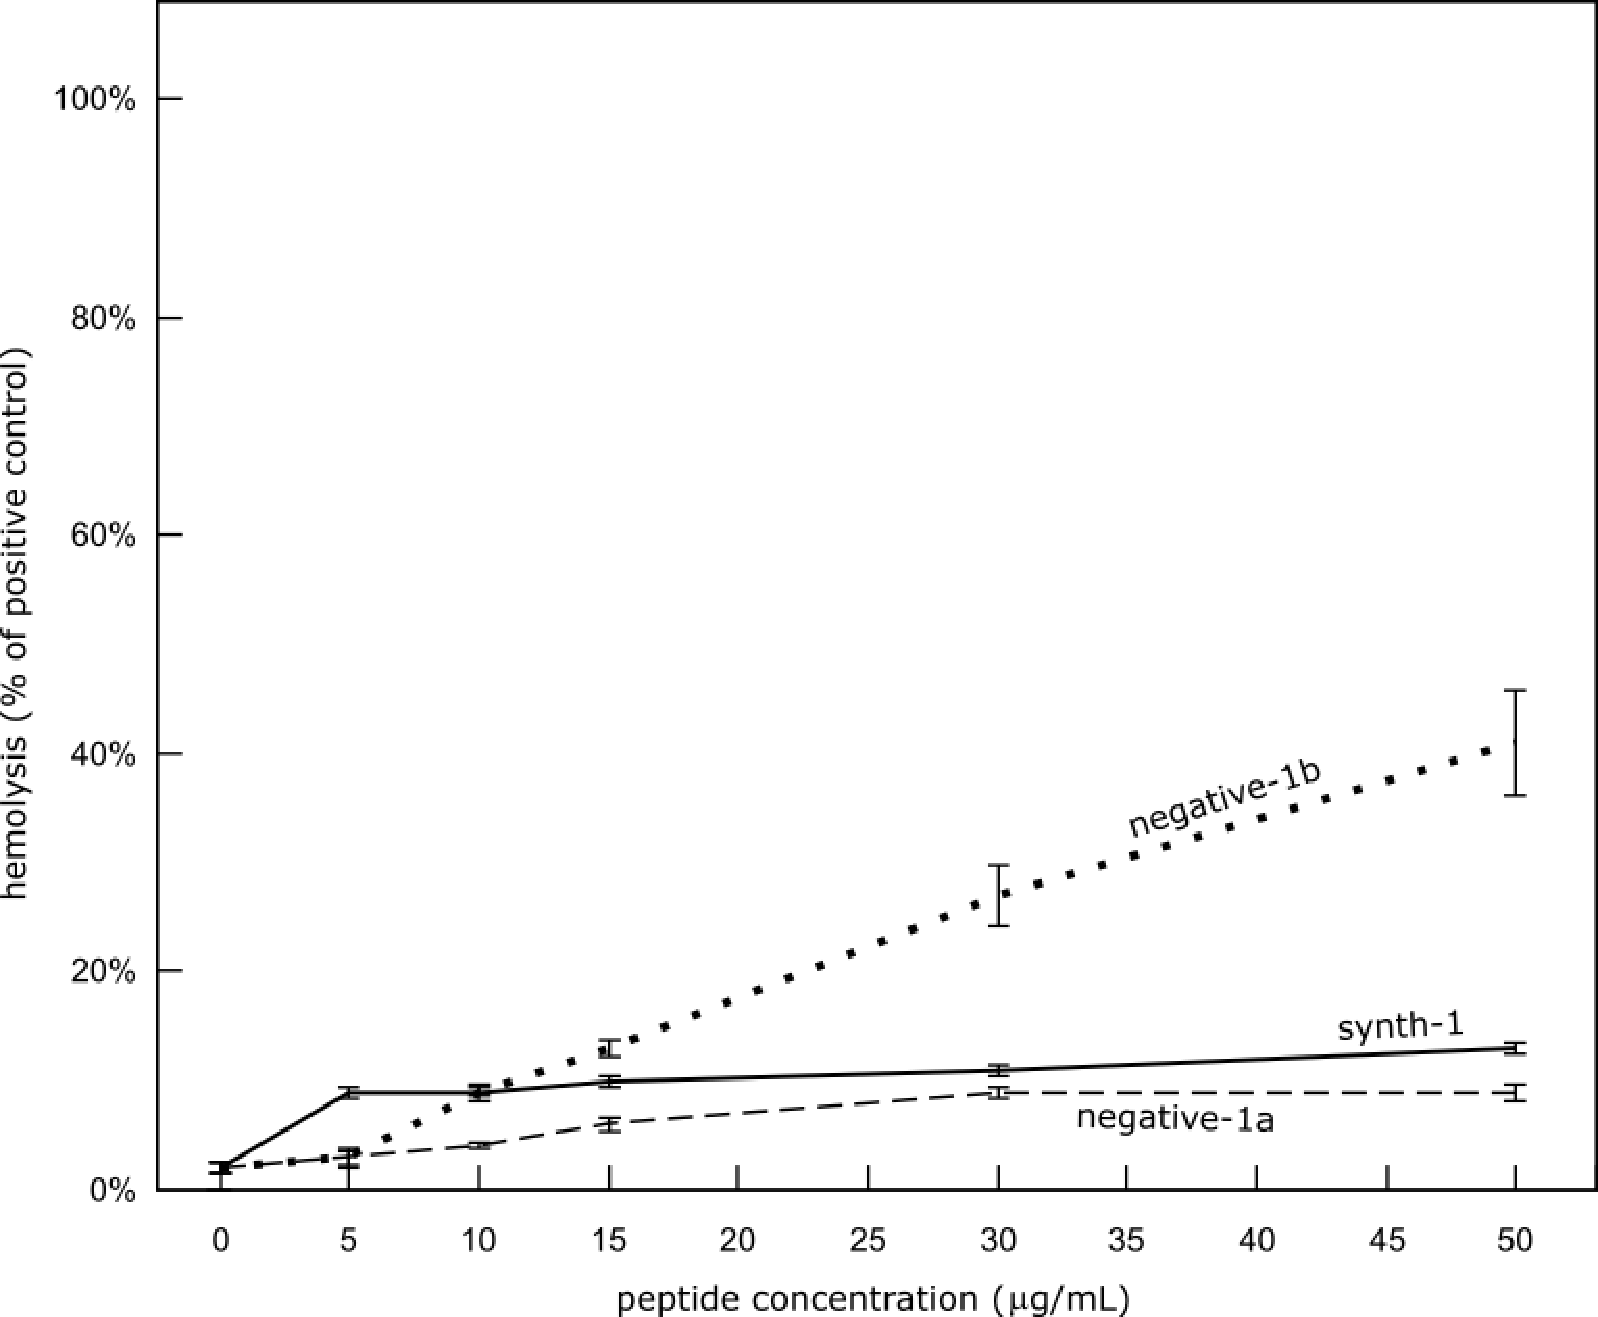
\includegraphics[width=0.95\textwidth]{Body/Images-chap2/hemolysis.pdf}
        \caption[Antimicrobial peptide hemolysis]{Activity
        of the synth--1 family of peptides against human
        erythrocytes determined using a procedure described
        elsewhere~\cite{liu2001denovo}.  The ordinate shows the
        degree of hemolysis relative to 50 $\mu$g/mL of melittin,
        which causes complete hemolysis.} \label{fig:hemolysis}
    \end{figure}





\subsection{Later experimentation}\label{section:fake}


    As mentioned briefly in the preceding sections, the experimental
    data suggesting that synth--1 had to antimicrobial activity,
    were later shown not to be reproducible.  Specifically, the
    *synth--1 peptide was shown to have no antimicrobial activity up
    to 50 $\mu g/mL$.  These experiments implied that the data for
    all of the synthetically generated peptides discussed in the
    previous section were suspect, with the exception of the data on
    the hemolytic potential of the peptides.  Based on these new
    findings, we revisited the AmP design problem and developed a
    more focused approach on the assumption that the original
    evolutionary methodology would not succeed.  In particular, the
    lack of activity by the *synth--1 peptide indicated that perhaps
    the $Z$--score was an inadequate metric for designing AmPs,
    despite its power for annotation.


\section{Focused design of AmPs}\label{section:focused}

\subsection{Derivation of highly conserved AmP grammars}

    In the previous section, I described a strategy for designing
    novel AmPs that have a strong emphasis on sensitivity.  That is,
    much effort was expended collecting a database of AmP sequences
    that was exhaustive so that the set of grammars derived from
    that database would be exhaustive as well
    (see Section~\vref{section:annotation}).  The
    annotation experiments suggest that this strategy is sensitive
    for discovering novel AmPs; however, the lack
    antimicrobial activity by *synth--1 suggests that perhaps this
    approach (and the metric $Z$) is not selective.  This lack of selectivity may be
    rooted in the exhaustive database of AmP sequences, which
    contains many sequences spanning a wide range of
    activities.  That is, there are some AmP sequences in the
    database that have very low activity and some with very high
    activity.  In addition, many of the sequences in this database
    are in precursor form.  For the sequences, the precursor
    undergoes a series of post translational modifications before
    yielding a mature, active antimicrobial peptide.  The regions of
    the proteins that are cleaved off, or otherwise not responsible
    for the antimicrobial activity of the peptide are essentially
    ``noise'' in the derived set of $\sim$200K grammars derived in
    the previous section.

    In order to focus instead on specificity, not sensitivity \emph{per se}, we
    decided to use a database of well--characterized eukaryotic AmP
    sequences from the Antimicrobial Peptide Database
    (APD)~\cite{wang2004apd}.  The APD is unique in that it is the
    only database of antimicrobial peptides that restricts the
    sequences it catalogs to only those for which there is a large
    body of experimental data confirming the activity of each AmP.
    Furthermore, the AmPs listed in the APD are mature in the sense
    that they are not precursor proteins.  Therefore, we know with
    high confidence that each sequence in the APD  has
    antimicrobial activity and that we are unlikely to be training
    on sequences that are not responsible in some part for this activity.

    As in Section~\vref{section:preliminary},
    we used the Teiresias pattern
    discovery tool to derive regular grammars that occur commonly
    in the set of 526 well--characterized eukaryotic AmP
    sequences from the APD\@.
    Using these APD sequences, we ran the Teiresias pattern discovery
    tool with the following settings: L = 6, W =
    6, and K = 2 (a detailed description of the
    Teiresias input parameters and associated tools
    is available in Section~\vref{section:teiresias}). The resulting grammar
    set was masked from the input sequences and the
    process was repeated using L = 7, W = 15, K = 5
    with the following amino acid equivalency groups
    \texttt{[[AG], [DE], [FYW], [KR], [ILMV], [QN], [ST]]}.
    The equivalency groups mean that Teiresias will consider any two
    characters in the same group to be exactly equivalent.  Thus, in
    the groups above alanine is treated exactly as glycine.  In
    effect, using equivalency groups allows us to find motifs that
    are more weakly conserved, but that have similar chemistries.
    (As I will show in Chapter~\vref{chapter:gemoda}, Teiresias
    is unable to use a more fine--grained metric for the similarity
    between two amino acids.  That is, Teiresias can only use
    equivalency groups to say ``equivalent'' or ``not equivalent''
    but it cannot use metrics such as ``alanine is five arbitrary
    units in a way from glycine, which is 10 arbitrary units away
    from leucine.)

As I discussed in Section~\vref{section:teiresias}, Teiresias
outputs its grammars in regular expression format, using wildcards.
To make the grammars more selective, we de--referenced each wildcard
in the grammars to a bracketed expression, using the same procedure
described in Section~\vref{section:annotation}. That is, we replaced
each wildcard with the set of amino acids implied by the grammar's
offset list. Finally, as in Section~\ref{section:annotation}, to
allow partial matches as short as 10 amino acids, we divided each
grammar into sub--grammars using a sliding--window of size 10,
resulting in 1551 grammars of length ten.

By design, these 1551 are sensitive for the AmP sequences from the
APD\@.  That is, these sequences from the APD are likely to be
matched by the grammars.  However, the grammars are not necessarily
specific for the APD AmPs. That is, non--AmP sequences may also be
matched by the grammars.  As discussed above, in our revised
strategy, we used the APD sequences to enhance specificity.  Here,
we reinforce this specificity by eliminating noninformative
grammars.

To select only those AmP grammars that are both sensitive and
selective, we searched each of the grammars against the nearly
exhaustive set of all known AmPs that was assembled in
Section~\vref{section:annotation}. These sequences consisted of the
$\sim$750 AmPs from the AMSdb~\cite{tossi2002antimicrobial}, which
were supplemented with an additional $\sim$200 antimicrobial
peptides from Swiss--Prot/TrEMBL that were not included in the
AMSdb.  In addition, we searched each of the grammars against
sequences from Swiss--Prot/TrEMBL that were not AmPs.  Using these
two searches, we eliminated grammars that were not at least 80\%
selective for AmPs. That is, at least 80\% of the matches for a
single grammar had to come from the set of all known AmPs.

    The resulting, final set of 684 ten amino acid
    grammars was used as the basis set of grammars to design the unnatural AmPs.
    As before, we say that these ~700 grammars describe the ``language'' of
    the AmP sequences and any sequence that is matched by one of the
    grammars is, at least in part, ``grammatical.''


\subsection{Design of synthetic AmP sequences}

    To design unnatural AmPs, we combinatorially
    enumerated all grammatical sequences based on
    the set of $\sim$700 grammars.  First, for each grammar,
    we wrote out all possible grammatical amino
    acid sequences.  So, for example, for the grammar
    \texttt{[IVL]K[TEGDK]V[GA]K[AELNH][VA][GA]K} produced 600
    sequences, where 3*5*2*5*2*2 = 600, due to the
    option of choosing one of many amino acids at each
    bracketed position.  There are roughly 3 million
    such 10--mers that correspond to antimicrobial
    patterns.  Then we wrote out all possible 20 amino
    acid sequences for which each window of 10 amino
    acids is found in the set of 3 million 10--mers.

    This process is somewhat analogous to the convolution step of
    Teiresias.  That is, we have essentially ``stitched'' small
    grammatical sequences together to form longer grammatical
    sequences.  For example, the grammatical 10--mer
    \texttt{IKTVAKEVGK} would be stitched together with any other
    10--mer beginning with the nine amino acid sequence
    \texttt{KTVAKEVGK}.  In this way, the small set of $\sim$700
    grammars can give rise to a tremendous number of 20 amino
    acid sequences.

    From this set, we removed any 20--mers that had
    six or more amino acids in a row in common with
    a naturally occurring AmP.  There are roughly 12
    million such 20--mers, each of which is a ``tiling''
    of ten 10--mers.



In the last section (see page~\pageref{section:preliminary}), I
described a metric, $Z$, for scoring sequences against a database of
grammars.  Recall that $Z$ essentially is a measure of what fraction
of a query sequence is matched by grammars from the database of AmP
grammars.  However, this metric was not dependent upon how many
grammars matched the query sequence.  That is, there was no
weighting of grammars that were particularly common in AmPs relative
to grammars that may have only occurred once or twice.  Consistent
with the approach in the previous section, this metric is sensitive,
rather than specific.  In our new, more focused approach, we
developed a different metric $Q$, which is the degree to which a
given 20--mer is grammatical.  This score is computed by making a
sequence dot plot matrix~\cite{maizel1981enhanced} (see
Figure~\vref{fig:dot}).  In the dot plot, the columns represent the
positions, 1--20, of the query 20--mer and the rows represent the
concatenated sequences of the $\sim$1000 naturally occurring AmPs. A
dot is placed in the matrix wherever a grammar matches both a
naturally occurring AmP and the 20--mer.  Then score $Q$ is then
just the number of dots in the matrix.  That is, the score $Q$ is
the area shown at the bottom of Figure~\vref{fig:dot2}.  As shown in
the figure, the score $Q$ is more indicative of how homologous a
query sequence is to the naturally occurring AmPs than the score $Z$
developed in the previous section.  (Rather than the area under the
curve, the score $Z$ is just the fraction of the query that is
matched by grammars.)

        \begin{figure}[ptb]
        \centering
        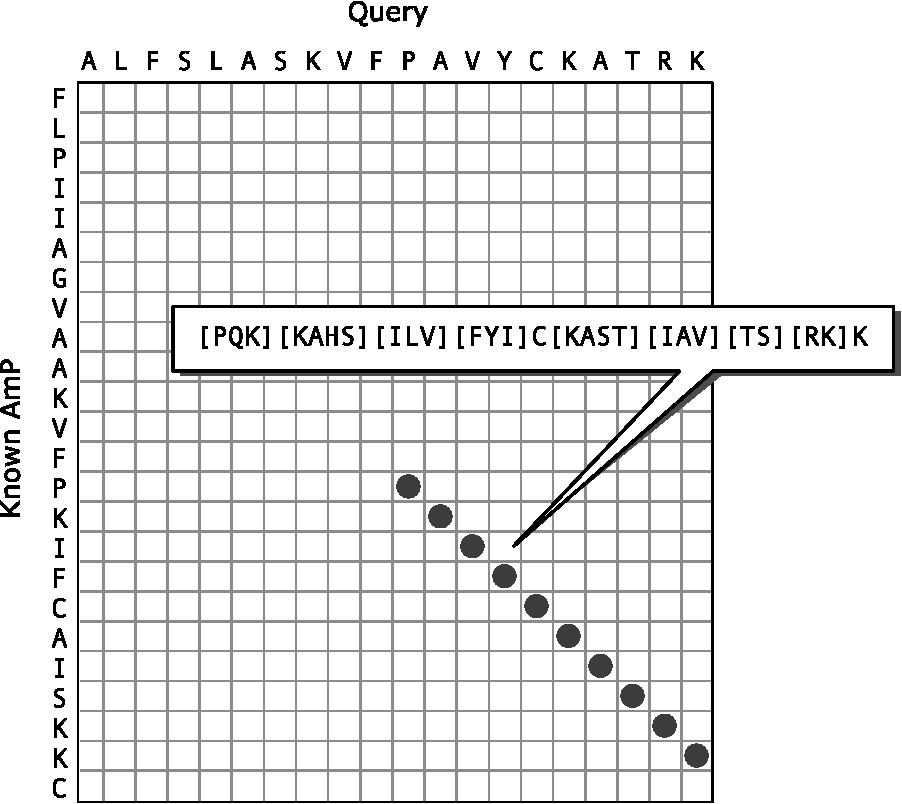
\includegraphics{Body/Images-chap2/dot.pdf}
        \caption[Example grammar--based dot plot]{
            An example grammar--based dot plot.  The
            figure shows a query sequence all the top and a single
            known AmP sequence on the vertical axis along the side.
            The matrix has an entry for each pair of amino acids
            between the two sequences.  The breakout shows a grammar
            from our database that matches both of the sequences.
            Note that both sequences begin a grammar with a proline
            residue; however, the grammar is not entirely conserved.
             The next residue in a grammar differs in each of the
             two sequences.  To calculate our scoring metric $Q$ we
             compute many grammar--based dot matrices using this same
             approach.  For example, see Figure~\vref{fig:dot2}.
            Activity of rationally designed AmPs.
        }
        \label{fig:dot}
        \end{figure}


        \begin{figure}[ptb]
        \centering
        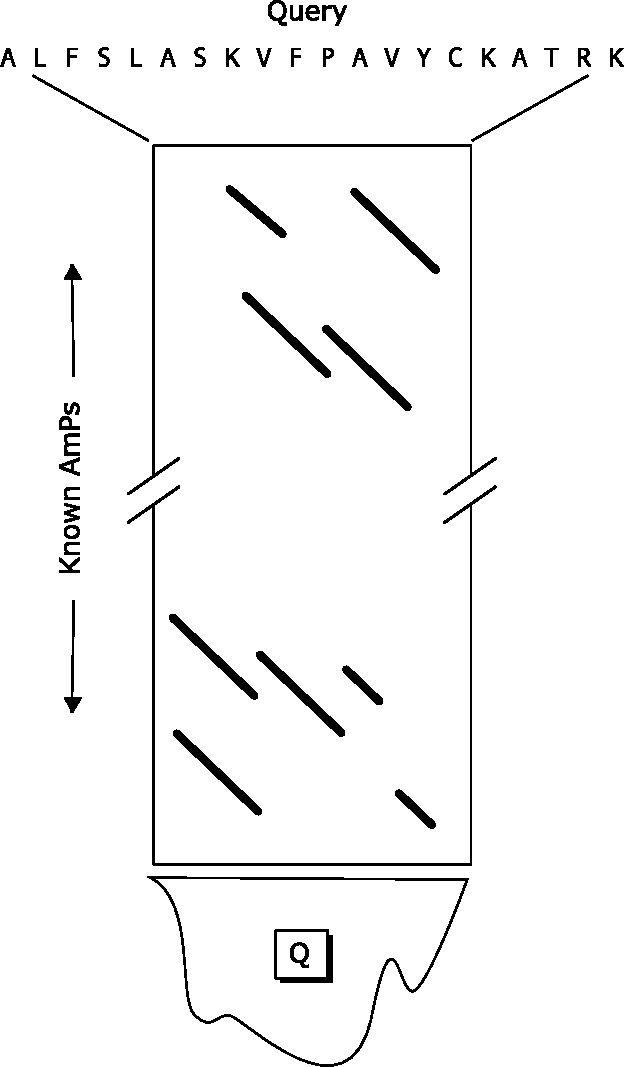
\includegraphics{Body/Images-chap2/dot2.pdf}
        \caption[Example  grammar--based dot plot for computing $Q$]{
            An example  grammar--based dot plot for computing $Q$.
            The figure shows a ``zoomed out'' view of many dot
            matrices concatenated together.  (See the dot matrix
            shown in  Figure~\vref{fig:dot}.)  At the top of the
            matrix is the query sequence, which is the synthetic,
            hypothetical AmP that is to be scored.  Along the
            vertical axis lay the concatenated sequences of the set
            of $\sim$900 known AmPs.  The diagonal streaks show
            places where a grammar matches both the query sequence
            and a known AmP.  At the bottom, to score $Q$ is shown.
            The score is the area under the curve and is simply a
            tally of the total number of dots in the dot matrix.
            War, equivalently, the total length of all streaks in
            the figure.  In this sense, the score $Q$ has a greater
            emphasis on specificity than did the score $Z$, which
            was merely be extent of the query sequence covered by
            grammars.
        }
        \label{fig:dot2}
        \end{figure}


In order to choose a representative set of sufficiently different
synthetic sequences to test experimentally, we clustered the 12
million sequences using the Mcd--hit
software~\cite{li2001clustering} at 70\% identity. From these
clusters, we chose 42 high scoring sequences to test experimentally.
These sequences have varying degrees of similarity to naturally
occurring AmPs, as determined by sequence alignment. Notably, from
each cluster, we took the highest scoring synthetic sequence based
on the $Q$ metric. These 42 sequences are shown in the left--hand
side of Table~\vref{table:chrisResults1}.

    For each of the 42 synthetic peptides, we also
    designed a shuffled sequence, in which the order
    of amino acids was rearranged randomly such that
    the sequence did not match any grammars. These
    shuffled peptides are shown in the right--hand side of Table~\vref{table:chrisResults1}.
    Necessarily, these peptides had the same amino acid
    composition as their synthetic counterparts and
    thus, the same molecular weight, charge, and pI:
    bulk physiochemical factors often correlated with
    antimicrobial activity.  We hypothesized that
    because the shuffled sequences were ``ungrammatical''
    they would have no antimicrobial activity,
    despite having the same bulk physiochemical
    characteristics. In addition, we selected  9
    peptides from the APD as positive controls (Cecropin P1, Cecropin
Melittin Hybrid, Cecropin--A Magainin 2 Hybrid, Melittin, Magainin
2, Hepcidin, Pyrrhocoricin, Ranalexin, and Parasin) and
    six 20--mers selected randomly from the middle of non--antimicrobial proteins as
    negative controls.


\subsection{Assay for antimicrobial activity}

Each of the peptides shown in Table~\vref{table:chrisResults1} was
synthesized using solid--phase, Fmoc chemistry on an Intavis
Multipep Synthesizer (Intavis LLC, San Marcos, CA) at the MIT
Biopolymers Lab. Mass spectrometry was used to confirm the accuracy
of the synthesis --- typical purities obtained with the synthesizer
were $>$85\%.

    We characterized the activity of each synthetic
    AmP using a broth microdilution assay described
    elsewhere~\cite{wu1999interaction}.  This assay measures the
    MIC at which the
    peptide inhibits growth of the target organism.
The assay is based on the NCCLS M26A and the Hancock assay for
cationic peptides (Hancock, NB, Canada). Briefly, serial dilutions
of peptides in 0.2\% Bovine Serum Albumin and 0.01\% Acetic acid
were made at 10x the desired testing concentration.  Target bacteria
were grown in Mueller Hinton Broth (BD, Franklin Lakes, NJ) to OD600
between 0.1 to 0.3 and diluted down to $2-7\times10^5$ cfu/mL in
fresh MHB, as confirmed by plating serial dilutions.  Five $\mu$L of
the peptide dilutions was incubated with 45 $\mu$L of the target in
sterile, capped, polypropylene strip tubes for 16--20 hours.  The
minimum concentration that prevented growth based on visual
inspection of OD was defined as the MIC.  When desired, the samples
that did not grow were streaked on an MHB agar plate to see if the
peptide was bacteriocidal.

Recombinantly produced standards for Cecropin P1, Cecropin Melittin
Hybrid, Melittin, Magainin 2, and Parasin were purchased from the
American Peptide Company (Sunnyvale, CA).   In antimicrobial assays,
four of the five recombinant peptides had identical activities to
the chemically synthesized versions from MIT biopolymers, with the
last being one dilution different (Cecropin P1).

\subsection{Results and conclusions}
    Table~\vref{table:chrisResults1} shows the MICs of synthetic peptides
    against \emph{B. cereus} and \emph{E. coli},
    as representative gram positive and gram negative
    bacteria.  (Two of the designed and 4 shuffled
    peptides were insoluble).  Of the 40 soluble
    designed peptides, 18 had activity against at least
    one of the bacterial targets at 256 $\mu$g/ml or less.
    Only 2 of the soluble shuffled peptides displayed
    activity.  Thus, the activity is not an artifact
    of molecular weight, charge, or pI.

\begin{table}[ptbh]
    \caption[Antimicrobial activity of rationally designed and shuffled peptides]{Antimicrobial activity of rationally designed and shuffled peptides.
    Each entry shows the minimum inhibitory concentration in $\mu$g/mL\@.  ``+'' = MIC greater than 256 $\mu g/mL$.  ++ = MIC greater than 128 $\mu g/mL$, not sufficiently soluble to test at 256 $\mu g/mL$.}\label{table:chrisResults1}
                \centering \scriptsize
        \begin{tabular}{llcclcc} \hline\hline
Peptide  &  Sequence  &  \emph{E. coli}  &  \emph{B. subtilis}  &  Shuffled Sequence  &  \emph{E. coli}  &  \emph{B. subtilis} \\
\rowcolor[gray]{0.9}
1  &  \texttt{ALFSLASKVVPSVFSMVTKK}  &  +  &  +  & \texttt{MVVFSVPKFKSTVAKLLSSA}  &  +  &  + \\
2  &  \texttt{VVFRVASKVFPAVYCTVSKK}  &  128  &  +  & \texttt{TAKVVVFVSFSYVVPKKRAC}  &  +  &  + \\
\rowcolor[gray]{0.9}
5  &  \texttt{FLFGLASKVFPAVYCKVTRK}  &  64  &  256  & \texttt{FLPVLVKVFRYSKKTAAGCF}  &  ++  &  64 \\
6  &  \texttt{LSAVGKIASKVVPSVIGAFK}  &  +  &  +  & \texttt{GVSSPIVAVKFKGAVASLIK}  &  +  &  + \\
\rowcolor[gray]{0.9}
7  &  \texttt{PVIGKLASKVVPSVFSMIKR}  &  +  &  +  & \texttt{SRVPLKSPVKIVGSKVMIFA}  &  +  &  + \\
9  &  \texttt{GLMSLVKDIAKLAAKQGAKQ}  &  256  &  +  & \texttt{GLKKDALQSIVKKAQLAAMG}  &  +  &  + \\
\rowcolor[gray]{0.9}
15  &  \texttt{SALGRVASKVFPAVYCSITK}  &  +  &  +  & \texttt{LYSPTCVKAAVSRFIGKVSA}  &  +  &  + \\
22  &  \texttt{LGALFRVASKVFPAVISMVK}  &  256  &  64  & \texttt{SVPSVGAVLFFKRAAVMKLI}  &  +  &  + \\
\rowcolor[gray]{0.9}
23  &  \texttt{ALGKLASKVFPAVYCTISRK}  &  128  &  +  & \texttt{KYGPALVIAVKKSCSLTFRA}  &  +  &  + \\
24  &  \texttt{GFIGKLASKVVPSVYCKVTG}  &  128  &  +  & \texttt{GGSTLGVFVKKSKACVIVPY}  &  \multicolumn{2}{c}{Not  soluble}     \\
\rowcolor[gray]{0.9}
25  &  \texttt{PVVFSVASKVVPSLISALKR}  &  +  &  +  & \texttt{KSPFVLVVSSRVAAVIKSLP}  &  +  &  + \\
28  &  \texttt{FLGVVFKLASKVFPAVFGKV}  &  64  &  16  & \texttt{GVSVAGAKKVKVLFVFPFLF}  &  +  &  + \\
\rowcolor[gray]{0.9}
29  &  \texttt{PAVFKIASKVVPSVYCKVSR}  &  128  &  +  & \texttt{KVYVVKIAVPCFPKSARSVS}  &  +  &  + \\
30  &  \texttt{GALFGLASKVFPAVFGAFKK}  &  256  &  +  & \texttt{KVVLFGAAGAKLFKASFFGP}  &  \multicolumn{2}{c}{Not enough material}   \\
\rowcolor[gray]{0.9}
31  &  \texttt{SAVGKLASKVFPAVFSMVTK}  &  +  &  +  & \texttt{FMKVLAVFGSVVTSAPKASK}  &  +  &  + \\
33  &  \texttt{VKDLAKFIAKTVAKQGGCYL}  &  ++  &  ++  & \texttt{ALVYAGIKKTAFLKVQKCDG}  &  +  &  + \\
\rowcolor[gray]{0.9}
34  &  \texttt{GVVGKLASKVVPSVFGSFTK}  &  +  &  +  & \texttt{SVKPVGSSVVKGTALVKFFG}  &  +  &  + \\
35  &  \texttt{LPVVFRVASKVFPALISKLT}  &  +  &  256  & \texttt{KVFIATLVVSSFLLAKPPRV}  &  +  &  + \\
\rowcolor[gray]{0.9}
36  &  \texttt{SAVGSVASKVVPSLISKVTK}  &  +  &  +  & \texttt{STVKVASKLAVVVSPISKGS}  &  +  &  + \\
39  &  \texttt{MKSIAKFIAKTVAKQGAKQG}  &  +  &  +  & \texttt{AKKAQKSGAQTIVKIFAKGM}  &  +  &  + \\
\rowcolor[gray]{0.9}
42  &  \texttt{LPAVFKLASKVVPSVFGLVK}  &  +  &  +  & \texttt{VVAKKFFVLVKGLAPVLSPS}  &  +  &  + \\
43  &  \texttt{SFVFKLASKVVPSVFSALTR}  &  256  &  256  & \texttt{ASPTVFRSSVFLSLFVVAKK}  &  +  &  + \\
\rowcolor[gray]{0.9}
44  &  \texttt{SVIGKIASKVVPSVYCAISK}  &  +  &  +  & \texttt{IASAVPVCVKGKISKSYISV}  &  +  &  + \\
45  &  \texttt{PVVGRVASKVFPAVIGLVKK}  &  +  &  +  & \texttt{VKRAGKGVAVVPSPLFKIVV}  &  +  &  + \\
\rowcolor[gray]{0.9}
51  &  \texttt{FLFRVASKVFPALIGKFKKK}  &  64  &  16  & \texttt{RKVAPALIKSFVFLFKFKKG}  &  +  &  + \\
55  &  \texttt{LSFVGRVASKVVPSLISMIK}  &  256  &  +  & \texttt{SSSIPIKMVLVRALVFVKSG}  &  +  &  + \\
\rowcolor[gray]{0.9}
56  &  \texttt{SALGRLASKVVPAVIGKVTT}  &  +  &  +  & \texttt{TLVGVVAKLVATKIGSSPRA}  &  +  &  + \\
57  &  \texttt{LGVVGSLASKVVPAVISKVK}  &  +  &  +  & \texttt{PKVVGLSIVVVKAKVSSALG}  &  +  &  + \\
\rowcolor[gray]{0.9}
62  &  \texttt{LPAVFKLASKVFPAVYCKAS}  &  128  &  +  & \texttt{PSLLYKAKAVFCKPSAVAVF}  &  ++  &  ++ \\
63  &  \texttt{LPVLFKLASKVFPAVFSSLK}  &  256  &  64  & \texttt{VSVKKVLPFAPLKSLLSFAF}  &  256  &  256 \\
\rowcolor[gray]{0.9}
65  &  \texttt{VVGRVASKVVPSLIGLFTTK}  &  +  &  +  & \texttt{FKVVISKPGLSVRVGTALVT}  &  ++  &  ++ \\
69  &  \texttt{SVVFGVASKVVPSVIGKVKT}  &  +  &  +  & \texttt{VFSVKGGKPSVVIKVVVAST}  &  +  &  + \\
\rowcolor[gray]{0.9}
75  &  \texttt{FLPFVGRIASKVVPSVIGKV}  &  +  &  +  & \texttt{SKFPLAGIFSVPGVKRVVVI}  &  +  &  + \\
77  &  \texttt{GKKLAKTIAKEVAKQGAKFA}  &  64  &  +  & \texttt{VIAFAKTKEAKAKLKGQAKG}  &  +  &  + \\
\rowcolor[gray]{0.9}
81  &  \texttt{PFVGRVASKVVPSVYCAITR}  &  \multicolumn{2}{c}{Not  soluble}  &  \texttt{PAVYKSIVGFSPVARVTVCR}  &  \multicolumn{2}{c}{Not  soluble}   \\
82  &  \texttt{FVGSLASKVVPSVFGAIKTK}  &  +  &  +  & \texttt{KTVPVVLKASIKVSSAGFGF}  &  +  &  + \\
\rowcolor[gray]{0.9}
83  &  \texttt{LPVVFKIASKVVPSVISKIT}  &  +  &  +  & \texttt{KIVKVITVKSISPASLVPVF}  &  ++  &  ++ \\
84  &  \texttt{GAVFGVASKVVPSVFSAIKK}  &  +  &  +  & \texttt{SVKVAKSVIPSAVFAGGKVF}  &  +  &  + \\
\rowcolor[gray]{0.9}
85  &  \texttt{FVGGVASKVVPSVYCKVSKK}  &  +  &  +  & \texttt{KVGKGSYPCSFVKVVAKVSV}  &  +  &  + \\
88  &  \texttt{VVFKLASKVVPSVYCTITKK}  &  256  &  +  & \texttt{VKTKCSVPAVVYILVKTFKS}  &  +  &  + \\
\rowcolor[gray]{0.9}
96  &  \texttt{GALFSLASKVVPAVIGLIKK}  &  256  &  +  & \texttt{LPVLFSSAIAKVGIKLGAKV}  &  +  &  + \\
\hline\hline
\end{tabular}
\end{table}

\begin{table}[ptbh]
    \caption[Antimicrobial activity of rationally designed and shuffled peptides against
        \emph{S. aureus} and \emph{B. anthracis}]{Antimicrobial activity of rationally designed and shuffled peptides against
        \emph{S. aureus} and \emph{B. anthracis}.
    Each entry shows the minimum inhibitory concentration in $\mu$g/mL\@.   ``+'' = MIC greater than 256 $\mu g/mL$.  ++ = MIC
greater than 128 $\mu g/mL$, not sufficiently soluble to test at 256
$\mu g/mL$.}
            \label{table:chrisResults2}
                    \centering \scriptsize
            \begin{tabular}{llcclcc} \hline\hline
Peptide &  Sequence  &  \emph{S. aureus}  &  \emph{B. anthracis}   &  Shuffled Sequence  &  \emph{S. aureus}  &  \emph{B. anthracis} \\
\rowcolor[gray]{0.9}
28  &  \texttt{FLGVVFKLASKVFPAVFGKV}  &  8  &  16  & \texttt{GVSVAGAKKVKVLFVFPFLF}  &  +  &  + \\
51  &  \texttt{FLFRVASKVFPALIGKFKKK}  &  16  &  16  & \texttt{RKVAPALIKSFVFLFKFKKG}  &  128  &  256 \\
\rowcolor[gray]{0.9}
22  &  \texttt{LGALFRVASKVFPAVISMVK}  &  64  &  64  & \texttt{SVPSVGAVLFFKRAAVMKLI}  &  +  &  + \\
63  &  \texttt{LPVLFKLASKVFPAVFSSLK}  &  128  &  128  & \texttt{VSVKKVLPFAPLKSLLSFAF}  &  +  &  + \\
\rowcolor[gray]{0.9}
5  &  \texttt{FLFGLASKVFPAVYCKVTRK}  &  256  &  128  & \texttt{FLPVLVKVFRYSKKTAAGCF}  &  +  &  + \\
43  &  \texttt{SFVFKLASKVVPSVFSALTR}  &  256  &  128  & \texttt{ASPTVFRSSVFLSLFVVAKK}  &  +  &  + \\
\rowcolor[gray]{0.9}
35  &  \texttt{LPVVFRVASKVFPALISKLT}  &  256  &  128  & \texttt{KVFIATLVVSSFLLAKPPRV}  &  +  &  + \\
\hline\hline
\end{tabular}
\end{table}


    Of the the negative controls --- 6
    peptides randomly selected from the middle of
    non--antimicrobial proteins from Swiss--Prot/TrEMBL
    --- none had activity.  Six of the nine
    naturally--occurring AmPs in the positive control
    group show activity and one was insoluble.


Two of the designed peptides, D28 (FLGVVFKLASKVFPAVFGKV) and D51
(FLFRVASKVFPALIGKFKKK), inhibited \emph{B. cereus} growth at 16
$\mu$g/mL, which is close to the MICs of the strong positive
controls melittin and cecropin--melittin hybrid (8 $\mu$g/mL). (Here
we use the letter ``D'' to distinguish a designed peptide from its
shuffled equivalent with the same number.)  Peptides with gram
positive activity are particularly exciting because of the
prevalence of drug--resistant nosocomial \emph{S. aureus} and the
threat of bioterror agents such as \emph{B. anthracis}, or anthrax.
Therefore, we assayed the seven designed peptides that had gram
positive activity, including the highly active D28 and D51 peptides,
against the Smith Diffuse strain of \emph{S. aureus} and the Sterne
strain of \emph{B. anthracis}. As shown in
Figure~\vref{fig:barActivity}, all seven peptides had activity
against both bacteria, whereas only one of the seven shuffled
controls had activity.  Moreover, two designed peptides, D28 and
D51, had activity against \emph{Bascillus antrhracis} at 16
$\mu$g/mL, which is equivalent to the activity of cecropin--melittin
hybrid, a strong natural peptide.

Also, D28 was synthesized by MIT biopolymers 4 separate times and
the resulting peptides had consistent activities against both
\emph{E. coli} and \emph{B. cereus}.



        \begin{figure}[ptb]
        \centering
        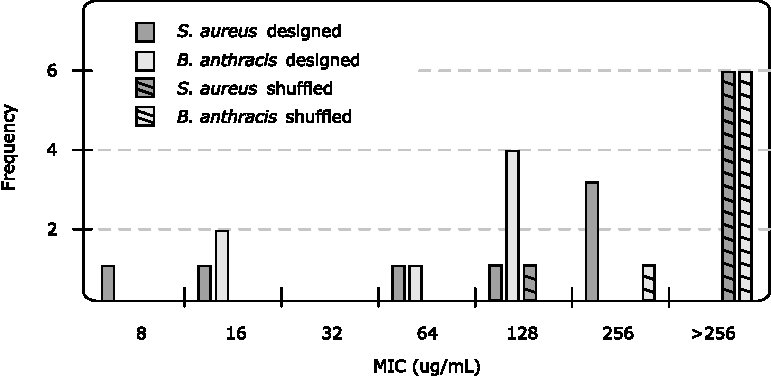
\includegraphics{Body/Images-chap2/barActivity.pdf}
        \caption[Activity of rationally designed AmPs against
        \emph{S. aureus} and \emph{B. anthracis}]{
            Activity of rationally designed AmPs against
        \emph{S. aureus} and \emph{B. anthracis}.  The figure shows
        that shuffled peptides (the hashed bars) tend to be grouped
        on the right side of the plot, indicating that they have
        little or no antimicrobial activity.  Only one of the
        shuffle peptides shows activity; however, it appears
        twice on the plot, once  at 128 $\mu$g/mL against
        \emph{S. aureus} and once act 256  $\mu$g/mL against \emph{B.
        anthracis}.  In contrast, all of the designed peptides show
        some degree of activity.  The most highly active peptide is
        that the left--hand side of the plot.
        }
        \label{fig:barActivity}
        \end{figure}

In an attempt to generate strong, synthetic AmPs, we
    optimized our best candidate, peptide D28, using
    a heuristic approach.  We created 44 variants of
    D28 by introducing mutations that were selected to
    increase positive charge, increase hydrophobicity,
    remove an interior proline residue, and improve
    segregation of positive and hydrophobic residues
    based on a helical projection.  16 of the 44 D28
    variants showed improved activity against \emph{E. coli}
    or \emph{B. cereus}.  All of the D28 variants with
    improved activity against \emph{B. cereus} included
    a mutation at an internal proline, either to
    lysine or glycine.  D28 and six of its variants
    were assayed for bacteriocidal activity, and
    all had activity within a 2--fold dilution of
    their MIC\@.  One variant had MICs of 16 $\mu$g/mL
    against \emph{E. coli} and 8 $\mu$g/mL against \emph{B. cereus}
    (relative to 64 and 16 $\mu$g/mL, respectively, for
    D28).

    We suspect that our linguistic approach to
    designing synthetic AmPs is successful due to the
    pronounced modular nature of naturally--occurring
    AmP amino acid sequences. As we have shown, this
    approach can be used to rationally expand the AmP
    sequence space without using structure--activity
    information or complex folding simulations. The
    peptides designed in this work are different from
    previously designed synthetic AmPs~\cite{tossi2000amphipathic,tiozzo1998wide} in that
    they bear limited homology to any known protein,
    which may be desirable for AmPs used in clinical
    settings. Some critics argue that widespread
    clinical use of AmPs that are too similar to human
    AmPs will inevitably elicit bacterial resistance,
    compromising our own natural defenses and posing
    a threat to public health~\cite{bell2003arming}. We hope
that this approach will help to expand the diversity of known AmPs
well beyond those found in nature, possibly leading to new
candidates for AmP--based antibiotic therapeutics.  Our designed
AmPs show some degree of homology with natural AmPs  because the
grammars are based on native sequences.  Peptide D28, for example,
was matched by grammars derived from 11 natural AmPs including
brevinin, temporin, and ponericin.  However, Smith--Waterman
alignments of our designed peptides against all natural AmPs in the
Swiss--Prot/TrEMBL database reveal that the degree of homology is,
by design (see Methods), limited.  In particular, our two most
active peptides, D51 and D28, have 50 and 60\% sequence identity
with the nearest natural AmP, respectively.  Peptide D51 has 6
semi--conservative and 4 nonconservative substitutions relative to
its closest neighbor, Ponericin W5.  Our linguistic design approach
may be most valuable as method for rationally constraining a
sequence--based search for novel AmPs. Diverse leads generated by
our algorithms may be optimized using approaches described in the
literature~\cite{hilpert2005high-throughput}. But, the linguistic
approach described here has a number of limitations. First, sequence
families that are poorly conserved on an amino acid level would not
benefit from this approach. Second, we suspect that the small size
of AmPs is helpful. Due to the simple nature of regular grammars,
they would be less useful for designing larger proteins and, in
particular, proteins with complex tertiary or quaternary structures.


\begin{comment}
    However, this
    is purely serendipitous.  We did not discriminate between natural
    AmPs of varying activities when building our grammatical model,
    nor did we incorporate any metric of hemolysis into our model.
    Accordingly, if our approach is used to design AmPs for clinical
    uses, these features would have to be optimized for the candidate
    peptide~\cite{kondejewski2002optimization, cuervo1988magainins}.
\end{comment}

\appendix
\chapter{Tables}

\begin{table}
\caption{Armadillos}
\label{arm:table}
\begin{center}
\begin{tabular}{||l|l||}\hline
Armadillos & are \\\hline
our	   & friends \\\hline
\end{tabular}
\end{center}
\end{table}

\clearpage
\newpage

\chapter{Figures}

\vspace*{-3in}

\begin{figure}
\vspace{2.4in}
\caption{Armadillo slaying lawyer.}
\label{arm:fig1}
\end{figure}
\clearpage
\newpage

\begin{figure}
\vspace{2.4in}
\caption{Armadillo eradicating national debt.}
\label{arm:fig2}
\end{figure}
\clearpage
\newpage

%% This defines the bibliography file (main.bib) and the bibliography style.
%% If you want to create a bibliography file by hand, change the contents of
%% this file to a `thebibliography' environment.  For more information 
%% see section 4.3 of the LaTeX manual.
%\bibliographystyle{plainnat}
\bibliographystyle{abbrvnat}

\clearpage
%\addcontentsline{toc}{chapter}{Bibliography}
\bibliography{References/research-new}

\end{document}

